%Dissertation Template for Columbia University Ph.D. programs
%By Charles McNamara, 2016
%I posted this document under a CC0 public domain license -- do whatever you want with it!
%It's probably a good idea to review the university guidelines just so you know what you want your dissertation to look like. You can read about those guidelines at this site: http://gsas.columbia.edu/content/formatting-guidelines.
%Good luck writing your dissertation!




% This is the main document file for the dissertation. You should not include any of your actual chapters or other substantive writing in this file.
%First we have to set up the style and formatting of the pages.

\documentclass[letterpaper,12pt]{memoir} %The memoir class is great for longer works that use separate chapters. The Dissertation Office recommends 10-pt Arial or 12-pt Times New Roman. I use 12-pt for readability.

%Below are some LaTeX packages to include to make sure that your Unicode characters render correctly. This is especially important if your dissertation includes polytonic Greek!

%\RequireXeTeX %XeTeX allows you to use Unicode characters like polytonic Greek in your writing.
%\usepackage{fontspec} %Allows you to load fonts in XeTeX.
%\defaultfontfeatures{Mapping=tex-text} %Allows you to get pretty TeX ligatures in your writing.
%\usepackage{xunicode} %You need this for Unicode fonts to work properly.
%\usepackage{xltxtra} %Some extra font capabilities for XeTeX
\DisemulatePackage{setspace} %You need to use this package for "true MS Word" double-spacing.
\usepackage{setspace} %Allows you to set different spacing (double, etc.) throughout your writing.
% \usepackage{hyperref} % Use if you want hyperlinks in your table of contents



%\setmainfont{Times New Roman}
%\setmainfont{Linux Libertine O} %This is a really readable serif font. It renders polytonic Greek better than any other OpenType font I've found, including Times New Roman. I now use it for everything, including class handouts. Highly recommended for classicists.

\usepackage{enumitem} % To fix spacing of bullet point lists
\setlist{noitemsep} % or \setlist{nosep} for space around whole list

%\pagestyle{fancy}
\usepackage[utf8]{inputenc}
\usepackage{amsmath}
\usepackage{amsfonts}
\usepackage{amssymb}
\usepackage{hyperref}
\usepackage{graphicx}
\usepackage{caption}
\usepackage{subfig}
\usepackage{sidecap}
\usepackage{bm}


\usepackage{cleveref}
\crefformat{footnote}{#2\footnotemark[#1]#3}

\usepackage{float}
\usepackage{amsbsy}
\usepackage{mhchem}
\usepackage{xfrac}

\DeclareUnicodeCharacter{00A0}{ }
\setsecnumdepth{subsubsection}

\newcommand\figref[1]{Fig.\,\ref{#1}}
\newcommand\eqnref[1]{Eqn.\,\ref{#1}}
\newcommand\tabref[1]{Tab.\,\ref{#1}}
\newcommand\secref[1]{Sec.\,\ref{#1}}
\newcommand\appref[1]{App.\,\ref{#1}}
\newcommand\citeref[1]{Ref.\,\cite{#1}}
\newcommand\chapref[1]{Chap.\,\cite{#1}}
\newcommand{\radon}{\ce{^{222}Rn}}
\newcommand{\uranium}{\ce{^{238}U}}
\newcommand{\thorium}{\ce{^{232}Th}}
\newcommand{\krypton}{\ce{^{85}Kr}}
\newcommand{\radioxenon}{\ce{^{136}Xe}}
\newcommand{\doublebeta}{2$\nu \beta \beta$}
\newcommand{\dru}{$\textrm{events} / (\textrm{kg} \cdot \textrm{day} \cdot \textrm{keV})$}

%Here is some stuff on the bibliography. You want to keep your bibliography file in the same directory as this file.


%\usepackage[american]{babel} %Enables hyphenation and date formats according to American conventions. Change "american" to "british" (or another value) if you work outside the US.
%\usepackage[backend=bibtex8,style=authoryear,texencoding=utf8,bibencoding=utf8]{biblatex} %The command here uses biblatex to render your bibliography, and it tells biblatex to use Unicode fonts. You can change the style of your citations easily by changing the value for "style" -- I use authoryear-icomp which takes care of the id/ibid citations automatically. There are many styles available if you want to change it.
%I have tried to use biber instead of biblatex many times, but it's never worked properly for me. I use biblatex, but feel free to try biber instead. 

\usepackage[backend=bibtex8,style=ieee]{biblatex} 
\addbibresource{./bibliography.bib} %Your bibliography file. I use JabRef to keep track of my bibliography. Highly recommended, and free! You can use Zotero if you want, but I've had trouble exporting to .bib files from my Zotero database.
\setlength{\bibitemsep}{\baselineskip} %Skip lines between bibliography entries. Columbia requires that you skip a line between entries.



%Here you can set margins and other page formatting

\setlrmarginsandblock{3.175cm}{3.175cm}{*} %Left and right margin -- the dissertation office requires at least 1-inch margins
\setulmarginsandblock{2.54cm}{2.54cm}{*}  %Upper and lower margin -- same thing, at least 1-inch margins
\checkandfixthelayout %A function of the memoir class that finds the right number of lines per page and apparently tidies up the formatting in other mysterious ways...?

% penalize footnotes that run onto next page
\interfootnotelinepenalty=10000

% get rid of whitespace
\raggedbottom


% Below we start to set up the document itself, including how to use spacing throughout the dissertation.

\begin{document}

\sloppy %If I don't include sloppy, then Greek and Latin words screw up margins all over. If you don't include weird languages in your dissertation, you can probably leave this one out.
\chapterstyle{default} % Nice formatting for chapter headings. Check out the documentation for the memoir class for other options.
\footnotesep\baselineskip % Footnotes need to have a space between each one for Columbia's Dissertation Office. 
\setstretch{1.5} %Set line spacing to "true MS Word" double-spacing
%\setstretch{1.}
%\DoubleSpace % Use LaTeX double-spacing (more like 1.666 spacing)

\expandafter\def\expandafter\quote\expandafter{\quote\SingleSpace} %Keep all block quotes single-spaced regardless of body text spacing.
%\pagestyle{plain} %Put page numbers at the bottom-center for the whole dissertation. Columbia's dissertation office requires that the numbers appear at this location on the page throughout the document.
%\makeevenhead{plain}{\sffamily\leftmark}{}{\sffamily\rightmark}
%\makeoddhead{plain}{\sffamily\rightmark}{}{\sffamily\leftmark}

\makepagestyle{cu}
\copypagestyle{cu}{ruled}
	\makeevenfoot{cu}{}{\thepage}{}
	\makeoddfoot{cu}{}{\thepage}{}



%% Here's the Title Page
% This is the title page of my dissertation.
% You may need to change the text on this page for your particular department. Consult the Dissertation Office Formatting Guidelines.

\thispagestyle{empty} % No page number
\begin{center}
  \SingleSpace

  \vspace*{1in}

  [Title]

  \bigskip % Get space between title and author name

  [Title]

  \vspace{5in}

  Submitted in partial fulfillment of the\\
  requirements for the degree of\\
  Doctor of Philosophy\\
  in the Graduate School of Arts and Sciences

  \bigskip
  \bigskip

  COLUMBIA UNIVERSITY

  \bigskip % Get space between Columbia and the year

  2017
\end{center}


%% Here's the copyright page. I use a Creative Commons license.
% This is the copyright page of my dissertation.
% You might also consider using a Creative Commons license. Ask your adviser or the university's Copyright Office.

\thispagestyle{empty} % No page number
\null\vfill % Pushes Copyright to the bottom of the page.
\begin{center}
  \SingleSpace %Keep the Copyright single-spaced
© 2016\\
Matthew D Anthony\\
All rights reserved\\
\end{center}


%% Here's the Abstract
% This is the abstract of my dissertation.

\pagestyle{empty} % No page number in entire abstract
\begin{center}
  ABSTRACT

    Understanding Low-Energy Nuclear Recoils in Liquid Xenon for Dark Matter Searches and the First Results of XENON1T.

    Matthew Duschl Anthony
\end{center}

An abundance of cosmological evidence suggests that cold dark matter exists and makes up 83\% of the matter in the universe.  At the same time, this dark matter has eluded direct detection and its identity remains a mystery.  Many large international collaborations are actively searching for dark matter through its potential annihilation in high-density regions of the universe, its creation in particle accelerators, and its interaction with standard model particles in low-background detectors.

One of the most promising dark matter candidates is the weakly interacting massive particle (WIMP) which falls naturally out of extensions of the Standard Model.  A variety of detectors have been employed in the search for WIMPs, which are expected to scatter with atomic nuclei, yet none have been more successful than dual-phase liquid xenon time projection chambers (TPCs).  The first ton-scale liquid xenon TPC, XENON1T, began operating in 2016 and with only 34.2 days of data has set the most strict limits on the WIMP-nucleon interaction cross sections for WIMP masses above 10 GeV/$\textrm{c}^2$, with a minimum of \num{7.7e-47} $\textrm{cm}^2$ for 35 GeV/$\textrm{c}^2$ WIMPs.

One of the major keys to success for liquid xenon TPCs is our understanding of interactions in the medium through myriad measurements.  Given that the expected WIMP scattering rate increases with decreasing interaction energy, there has been more focus in recent years in pushing our understanding of interactions in liquid xenon to lower energies.  Additionally, as liquid xenon TPCs operate with a large electric field in the medium, an effort has been made to understand how the signal response of xenon changes as a function of the applied electric field.      
   
In this thesis, I describe the details of XENON1T, its calibration and characterization, with a special emphasis on the electronic and nuclear recoil calibrations, and the inaugural WIMP search of XENON1T.    I then discuss a dedicated measurement, made in the calibration-optimized liquid xenon TPC neriX, of the signal response of low energy nuclear recoils in liquid xenon at electric fields relevant to the dark matter search.  The measurements of signal response in XENON1T and neriX were performed using an analysis framework that I developed to allow a more sophisticated examination of recoil responses using GPU-accelerated simulations.




\maxtocdepth{subsubsection}

\frontmatter
\tableofcontents % You need to put your ToC after frontmatter so that it will get lowercase Roman numerals.
\cleardoublepage

%A list of graphs and illustrations should go here if you use any.
\listoffigures
\cleardoublepage

% Acknowledgements
% This is the acknowledgments page of my

\cleartorecto % A memoir-class command for moving the acknowledgments to a recto page, not verso.
\chapter{Acknowledgements} % For the heading on the page, also registers in the table of contents
\thispagestyle{plain} %This page should have numbers.



% Elena
First and foremost, I would like to thank my advisor, Elena Aprile.  Not only have you provided support and guidance throughout my time at Columbia but you have given me countless opportunities to learn and grow over my years in the group.  You have been such an inspiration to me and have been a phenomenal mentor.  I will also never forget how you took a chance on me in helping me transfer to Columbia and having me join your group --- I can honestly say that I would not be where I am today without you.


% Luke, Marc, and Guillaume
I would also like to give a special thanks to Luke Goetzke, Marc Weber, and Guillaume Plante for all of their help and guidance during my first few years at Columbia.  You all had seemingly infinite patience and I could not have asked for better teachers and role models.


% Postdocs
I would also like to thank all of the postdoctoral fellows and research scientists who taught, challenged, and mentored me over the course of my Ph.D.  Antonio Jesus Melgarejo Fernandez, Patrick de Perio, Marcello Messina, Qing Lin, and Fei Gao, you all have been an incredible inspiration and I cannot thank you enough for all of your support.  


% Grad Students
I would also like to thank my fellow graduate students Zach Greene, Yun Zhang, Joey Howlett, and Tianyu Zhu.  I have had so much fun working with you all over the years and I have learned so much from all of you and would not have succeeded without you.  


% Marcela
I would also like to give a special thanks to Marcela Stern.  It has been such a pleasure working with you and getting to know you over the years.  You are one of the kindest people I know and have made the last few years so enjoyable.


% Collaboration
I cannot thank my colleagues in the XENON collaboration enough for their hardwork and dedication that has made our joint effort such a success.  It has been a privilege to be part of such an extraordinary group of people.


% Physics Friends
I would also like to thank my friends Felix Clark, Zach Greene, Ryne Carbone, and Russell Smith.  It has been incredible to get to know you all over the last few years and it was so helpful to always have people to talk to and hang out or grab a beer with through the trials and tribulations of graduate school.  


% Parents
I am extremely grateful for my incredible and loving parents, Elizabeth and Robert.  You not only have been supportive of me in more ways than I can name but you instilled in me the virtues that have allowed me to get this far.  There is no way that I would be where I am today without your guidance and help and I owe you both a debt of gratitude that can never be repaid.  This achievement is as much yours as it is mine.



% Brothers and sisters, Beth and Steve, Haveners
I am also extremely thankful to my brothers and sisters: Alison, Alexandra, Halie, Kurt, Ryan, and Sara.  I would also like to thank my new parents, Georgiana and Henry, who have always been incredibly supportive throughout my studies and my ``New York parents'', Beth and Steve.  You all mean the world to me and your encouragement over the last five years has been so critical to me being able to push through and keep moving through the tough times.  I would like to give a special thanks to my brothers and best men Kurt and Ryan who have been a constant source of strength and inspiration --- I never would have made it this far without you.  


% Laura
Finally, I would like to thank my incredibly intelligent, talented, and beautiful wife, Laura.  Words cannot possibly describe how much you mean to me.  From our first summer doing research together, you have not just been an encouraging force but a source of inspiration.  You fought with me side-by-side through classes, the qualifying exams, and research and I never would have made it through without you.  I can never thank you enough for giving me the strength and confidence to get this far.  It is hard for me to think about closing this chapter together but I look forward to writing the rest of our story with you.  %It's sad to me that we're about to close this chapter of our lives but I look forward to writing the rest of our story.






% Dedication
% This is the dedication page of my dissertation.

\cleartorecto % A memoir-class command for moving the dedication to a recto page, not verso.
\thispagestyle{plain} % This page should be numbered

\begin{vplace}[0.7]
\begin{center}
  To my parents, Elizabeth and Robert, and my wife, Laura. \\
  \textit{If I have seen further it is by standing on the shoulders of giants.}
\end{center}
\end{vplace}

% Preface if you have one




%What follows is the main text of your dissertation. You can comment out lines if you want to exclude them from your document for drafts. Everything after \mainmatter will get Arabic numbers centered on the bottom of the page.

\mainmatter

%I use subdirectories for each part of my dissertation just to keep the files tidy. LaTeX generates a lot of different files for output, and using subdirectories allows you to find your .tex files more easily.

%This is the first chapter of the dissertation

%The following command starts your chapter. If you want different titles used in your ToC and at the top of the page throughout the chapter, you can specify those values here. Since Columbia doesn't want extra information in the headers and footers, the "Top of Page Title" value won't actually appear.
%\makepagestyle{cu}
%\copypagestyle{cu}{ruled}
%	\makeevenfoot{cu}{}{\thepage}{}
%	\makeoddfoot{cu}{}{\thepage}{}

\pagestyle{cu}
\graphicspath{{./Chapter1/images/}}

\chapter[Dark Matter][Dark Matter]{Dark Matter}

For nearly a century, experimental evidence has suggested that a large portion of the universe is made up of a non-luminous type of matter.  While this dark matter has only been detected indirectly via its interaction with normal matter through the gravitational force, recent experiments conclude that approximately 26\% of the entire energy density of the universe is comprised by dark matter.

	In this chapter, I will focus on the leading dark matter model, the experimental evidence for its existence, the different candidates for particle dark matter, and the current detection methods employed in the search for particle dark matter.
	
	
\section[$\Lambda$CDM Model][$\Lambda$CDM Model]{$\boldsymbol{\Lambda}$CDM Model}
\label{sec:cdm}

	One of the guiding principles of cosmology are the assumptions that the universe is both homogeneous and isotropic at large enough scales (typically on the order 100 Mpc or $10^{5}$ light years).  Continuing with these principles and maintaining generality, we can arrive at the Robertson-Walker space-time metric
	\begin{equation}
		ds = -c^{2}dt^{2} + a(t)^{2}\left( \dfrac{dr^{2}}{1 - kr^{2}} + r^{2}d\Omega^{2}\right)
	\end{equation}
Here, $a(t)$ is called the \emph{scale factor}, an arbitrary function of time allowing for time dependent changes of the universe, and $k$ is a constant modeling the curvature of the universe.  For $k=-1$, the universe is considered open, for $k=1$, the universe is considered closed, and at $k=0$ we are left with our Euclidean (flat) universe.  Note that for $a(t) = 1$ and $k = 0$ the Robertson-Walker metric reduces to the Minkowski metric.

	Using this metric in combination with Einstein's equation we can derive the equations for the Friedmann-Robertson-Walker universe described by the Friedmann equations.
	
	\begin{equation}
		\frac{\ddot{a}}{a} = -\frac{4 \pi G}{3} \left( \rho + 3p \right)
	\end{equation}
	\begin{equation}
		\left( \frac{\dot{a}}{a}\right)^{2} = \frac{8 \pi G}{3} \rho - \frac{k}{a^2}
	\end{equation}

	We can define several useful (and commonplace) parameters to simplify the second Friedmann equation further.
\\
\\
\textbf{Hubble Parameter}: $ H = \frac{\dot{a}}{a} $\\
\textbf{Critical Density}: $ \rho_{crit} = \frac{3H^2}{8 \pi G} $\\
\textbf{Density Parameters}: $ \Omega_{i} = \frac{8 \pi G \rho_i}{3H^2} = \frac{\rho_{i}}{\rho_{crit}} $\\
\begin{equation}
	\Omega - 1 = \frac{k}{H^2 a^2}, \ \ \ \ \Omega = \sum_{i} \Omega_{i} = \Omega_{\Lambda} + \Omega_{CDM} + \Omega_{Baryon} + \Omega_{Rad}  \ldots 
\end{equation}
	
Here the critical density is defined such that the universe is flat ($k=0$).  One can think of $\frac{\Omega_i}{\Omega}$ as what part of the total matter and energy budget a particular component makes up.  The main contributors to the density of the universe are dark energy and cold dark matter hence the $\Lambda$CDM Model.  The density parameters give insight into the large scale structure of the universe and measurements of the various density parameters and other $\Lambda$CDM parameters has been a major focus of research over the last two decades and will be discussed later in this chapter \cite{carroll1997lecture}.
	
\section{Evidence of Dark Matter}

\subsection{Dynamical Constraints from Clusters of Galaxies}

The first evidence of dark matter came from Fritz Zwicky in 1933.  Zwicky used a basic application of the virial theorem on galaxies in the Coma Cluster	to estimate the mass of the cluster.  He then  estimated the total mass based on the brightness of the cluster and found significant disagreement between the results leading him to the conclusion that ``if this would be confirmed we would get the surprising result that dark matter is present in much greater amount than luminous matter'' \cite{Zwicky1933}.
	
\begin{figure}[h]
\includegraphics[width=8cm]{coma_composite}
\centering
\caption{A composite image of the Coma Cluster combining X-ray data and optical data.  The gas in the cluster is shown in purple.  Image Credit: X-ray - NASA/CXC/MPE/J.Sanders et al, Optical - SDSS}
\end{figure}
	
	
\subsection{Dynamical Constraints from Galactic Rotation Curves}	
	
%\href{http://www.skyandtelescope.com/astronomy-resources/vera-rubin-dark-matter-detective/}{summary source}	

%\href{http://articles.adsabs.harvard.edu/full/1970ApJ...159..379R}{rubin paper source}	

\begin{figure}[b]
	\centering
	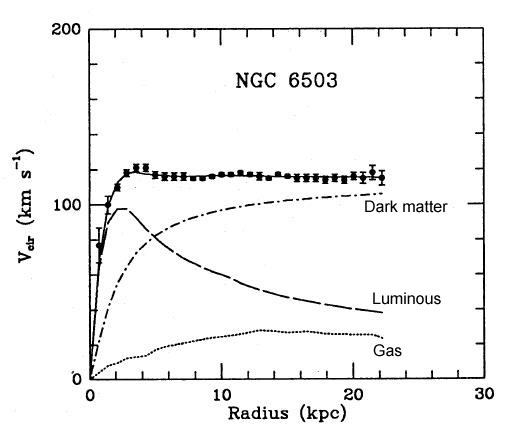
\includegraphics[width=8cm]{ngc_6503_rotation_curve}
	\caption{The rotation curve of the galaxy NGC 6503 broken down into individual components: visible matter (dashed), gas (dotted), and dark matter (dash dotted) \cite{Begeman1991}. }
	\label{fig:galactic_rotation_curve}
\end{figure}

	
Nearly fourty years later, stronger evidence was provided for the existence of dark matter by Vera Rubin and Kent Ford in their 1970 paper looking at the rotation curve of the Andomeda Galaxy \cite{rubin1970rotation}.  In this paper, Rubin used the H$\alpha$ lines to determine the orbital velocities of different stars in the galaxy.  Later measurements used the 21 cm hyperfine transition line to measure orbital velocities within other galaxies \cite{Begeman1991}.
	
	From simple Newtonian arguments, one gets the following description of the orbital velocity inside a galaxy:
	
\begin{equation}
v(r) = \sqrt{\frac{G M(r)}{r}}
\end{equation}	

In this equation, M(r) is the sum of all the mass within a radius $r$.  Under the assumption that most of the mass is concentrated at the center of the galaxy (in the form of a supermassive blackhole), one would expect that at large distances from the center of the galaxy, the orbital velocity would fall off as $v \propto r^{-1/2}$.

However, what is seen differs from this simple approximation drastically.  \figref{fig:galactic_rotation_curve} is taken from \citeref{Begeman1991} but the results are similar to what Rubin and Ford saw deecades earlier: the asymptotic behavior of the orbital velocity is constant and does not show any polynomial roll-off.  By isolating the contributions from measurable mass densities (such as visible matter and gas), one can get an idea of the density distribution of dark matter in a galaxy.  From the figure below, one could asymtotically estimate that $M(r) \propto r$ which would imply that $\rho(r) \propto r^{-2}$.  One quickly realizes that this cannot be the true density since the mass of the galaxy diverges but approximates the density within an effective radius.



\subsection{Evidence from Graviational Lensing}	

Gravitational lensing is the distortion of light coming from a source due to the warping of spacetime from the presence of large amounts of matter or energy.  This effect is illustrated in \figref{fig:gravitation_lensing_cartoon} and actually captured in the form of an Einstein Cross in \figref{fig:einstein_cross}.  In a gravitational lensing system, if we know the redshift (distance) of the source and the lense, we can estimate the gravitational field of the lensing system and hence its mass.


\begin{figure}[t]
	\centering
	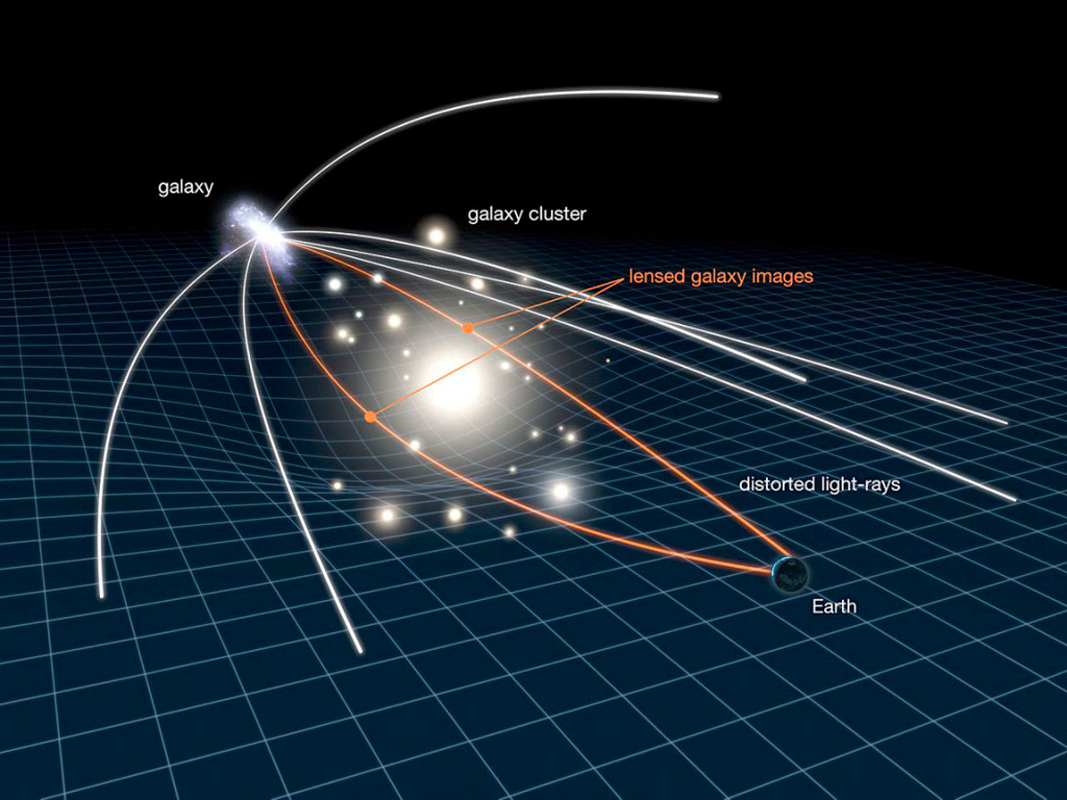
\includegraphics[width=0.8\textwidth]{gravitation_lensing_cartoon}
	\caption{A cartoon showing the deflection of light due to the warping of spacetime caused by the presence of a massive galaxy cluster.  Note that for very strong lensing, one expects multiple images of the source object and sometimes even an Einstein Ring around the lense. Image Credit: NASA/ESA.}
	\label{fig:gravitation_lensing_cartoon}
\end{figure}

\begin{figure}[t]
	\centering
	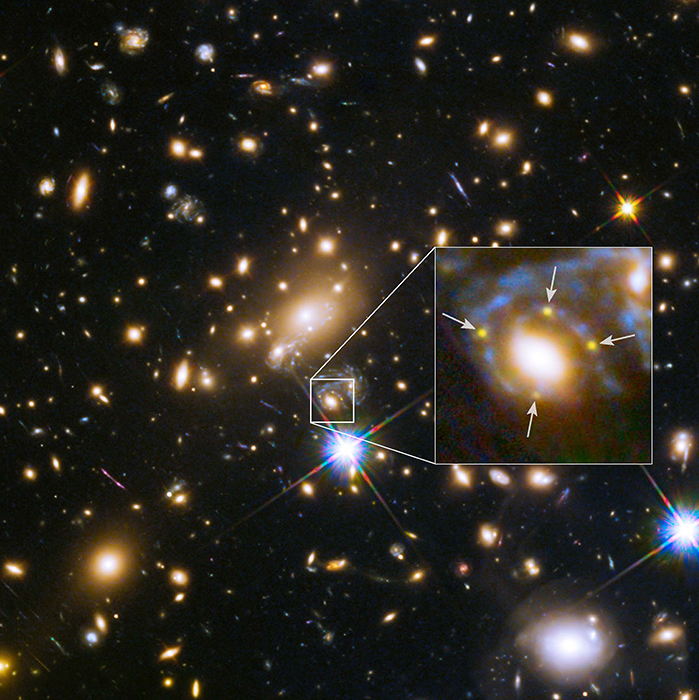
\includegraphics[width=0.8\textwidth]{einstein_cross}
	\caption{In this optical image you see the massive MACS J1149.6+2223 cluster.  In the zoomed portion, you can actually see the same supernova, SN Refsdal, in four smaller images around a large galaxy within the cluster. Image Credit: HST.}
	\label{fig:einstein_cross}
\end{figure}


%\begin{SCfigure}[\sidecaptionrelwidth][h]
%	\centering
%	\caption{In this optical image you see the massive MACS J1149.6+2223 cluster.  In the zoomed portion, you can actually see the same supernova, SN Refsdal, in four smaller images around a large galaxy within the cluster. Image Credit: HST.}
%	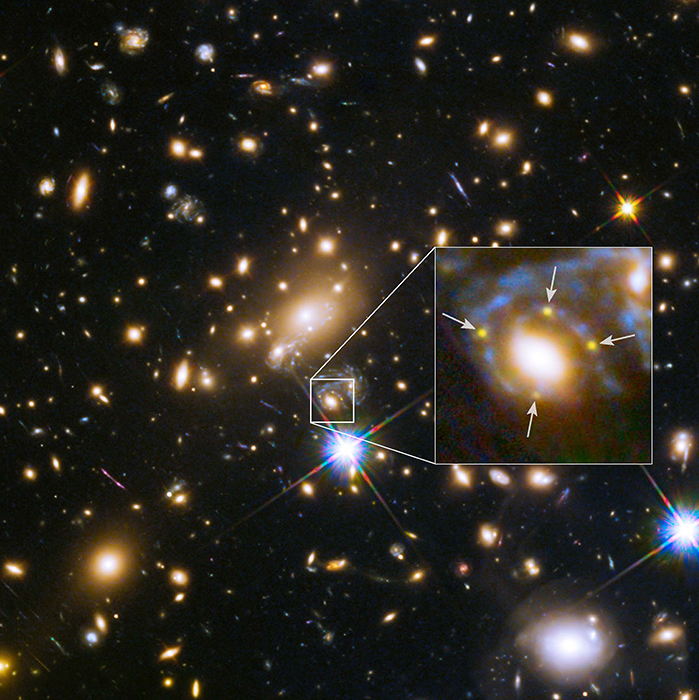
\includegraphics[width=0.5\textwidth]{einstein_cross}
%\end{SCfigure}

Mass estimation via gravitational lensing in itself is very useful for finding large discrepancies in mass from known sources and true mass (the discrepancy being attributed to dark matter).  However, when combined with x-ray measurements, as seen in \figref{fig:bullet_cluster}, one gets even more interesting results.  Shown in \figref{fig:bullet_cluster} is the Bullet Cluster (1E0657-558) which actually consists of two colliding sub-clusters.  In the image on the left, one can see the infrared image from Magellan that is used, along with optical images from Hubble, to estimate the mass distribution of each galaxy cluster through graviational lensing.  In the right image, one can see the X-ray map of the Bullet Cluster from the Chandra X-ray observatory with the same mass contours: one can see that the plasma from the clusters interacts giving the cone shapes in the center.  However, the mass contours largely remained centered on the individual clusters (as seen in the optical image) implying that the majority of the matter interacted minimally during the collision \cite{clowe2006direct}.  Since we know that the galaxies make up only a small fraction of the mass in a cluster from the virial theorem, this implies that the dark matter hardly interacts with itself or ordinary matter.

% https://astrobites.org/2016/11/04/the-bullet-cluster-a-smoking-gun-for-dark-matter/

\begin{figure}[t]
	\centering
	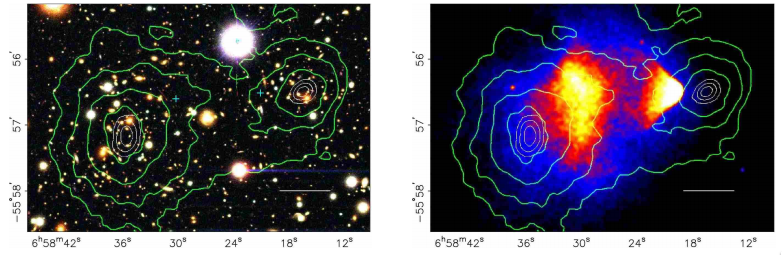
\includegraphics[width=0.999\textwidth]{bullet_cluster}
	\caption{Infrared (left) and X-ray (right) maps of the Bullet Cluster (1E0657-558).  While the plasma in the clusters interacts during the collision of the two individual clusters, as is seen by the shockwave in the center, the majority of the mass passes right through \cite{clowe2006direct}.}
	\label{fig:bullet_cluster}
\end{figure}


\subsection{Evidence from the Cosmic Microwave Background}

The Cosmic Microwave Background (CMB) has proven to be one of the richest discoveries in all of cosmology.  Accidentally discovered in 1964 by Penzias and Wilson \cite{penzias1965measurement}, the radiation from the CMB is almost perfectly isotropic and described by a blackbody spectrum at 2.725 K \cite{fixsen1996cosmic}.  The isotropy in the CMB provides the strongest evidence to date of the Big Bang Hypothesis and helped to formulate our current picture of the early universe down to the recombination epoch, where the universe was sufficiently cool such that hydrogen could form from the free electrons and protons in turn allowing photons to travel freely through the universe.  

\begin{figure}[ht]
	\centering
	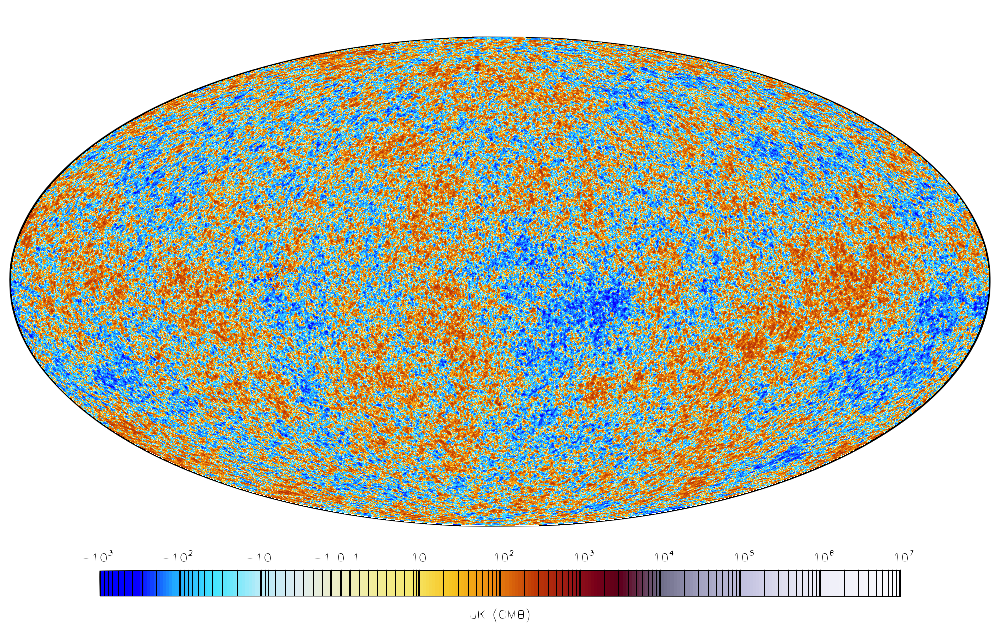
\includegraphics[width=0.95\textwidth]{planck_map}
	\caption{The Planck 2015 measurement of the temperature anisotropy of the CMB.  Note that the largest deviations from the mean are on the order of $200 \mu K$ from the 2.725 K mean (roughly 1 in $10^4$).  Image Credit: IRSA, \citeref{Ade2015}.}
	\label{fig:planck_map}
\end{figure}

\begin{figure}[ht]
	\centering
	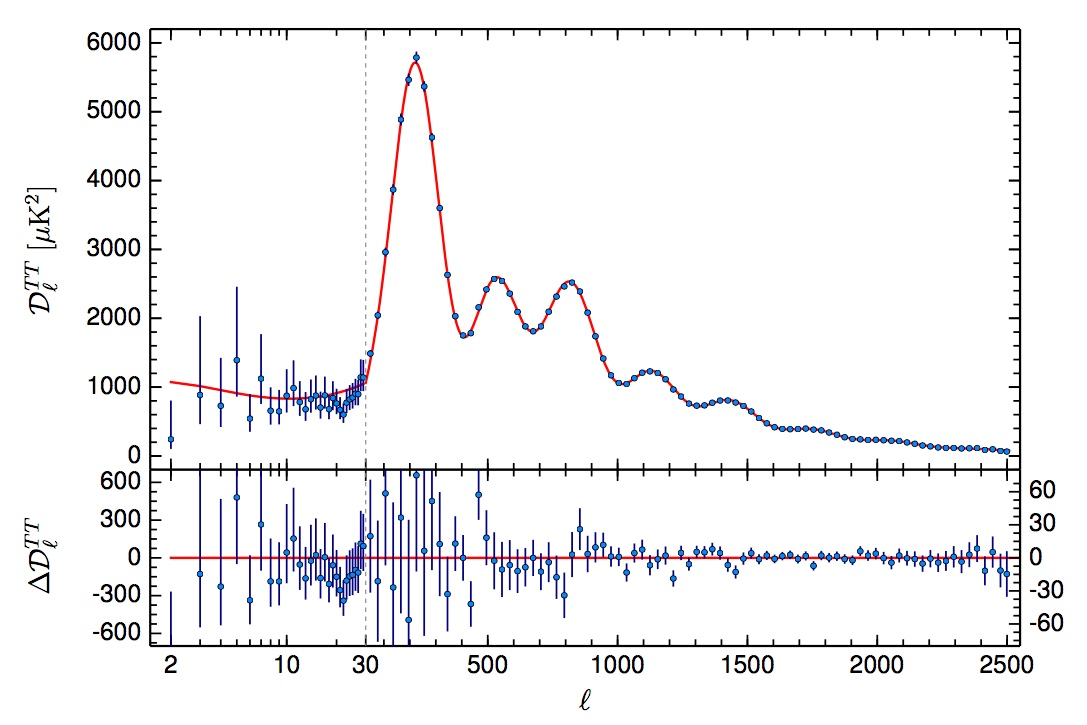
\includegraphics[width=0.95\textwidth]{planck_2015_power_spectrum}
	\caption{The power spectrum of the temperature anisotropies measured by Planck along with the best fit prediction from the $\Lambda$CDM model.  $\mathcal{D}_l^{TT}$ is a proxy for $C_i$ and is defined $\mathcal{D}_l^{TT} \equiv l(l+1)C_l / 2 \pi$.  Image Credit: \citeref{Ade2015}.}
	\label{fig:planck_fit}
\end{figure}

% https://www.astro.umd.edu/~miller/teaching/astr422/lecture21.pdf
% http://w.astro.berkeley.edu/~mwhite/rosetta/node2.html

As the CMB has been studied in more detail, cosmologists began to see that there are in fact very small temperature fluctuations on the order of ${\lesssim}100 \mu K$ \cite{bennett1996four, komatsu2011seven, Ade2015}.  These temperature fluctuations, as seen in the 2015 measurement of the CMB by the Planck satellite, are shown in \figref{fig:planck_map}.  To characterize the temperature fluctuations of the entire sky, we use the spherical harmonics, $Y_{lm}(\theta, \phi)$.  


\begin{equation}
	T(\theta, \phi) = \sum_{l=0}^{\infty} \sum_{m=-l}^{l} a_{lm} Y_{lm}(\theta, \phi)
\end{equation}

We assume that  the distribution of $a_{lm}$ should be described by a Gaussian distribution, as predicted by inflation, with a mean of 2.725 K for any given multipole moment $l$.  Therefore, the only piece missing to completely describe these $a_{lm}$ for each multiple moment is the variance of  this distribution so we define $C_l \equiv \left<| a_{lm}|^2\right>$.  These $C_l$ form the power spectrum of the CMB and can be used to test various formation models of the universe.  Planck tested the $\Lambda$CDM model described in \secref{sec:cdm} against their power spectrum (\figref{fig:planck_fit}) and found remarkable agreement between prediction and data while constraining some of the universal constants including $H_0$, $\Omega_{\Lambda}$, $\Omega_{CDM}$, $\Omega_{Baryon}$, and $\Omega_{Rad}$.  It is from this fit that we find that our universe has a curvature very close to zero and therefore is flat and that our universe is comprised of roughly  $~68.3\%$ dark energy, $~26.8\%$ dark matter, and $~4.9\%$ ordinary matter \cite{Ade2015}.

The $\Lambda$CDM model has been tested since its inception using N-body simulations to propagate the formation of large scale structure in the universe.  While small discrepancies between simulation and observation have been found, it is clear from these simulations that without cold dark matter it is extremely difficult to explain the large scale structure we see in the universe given the anisotropies of the CMB \cite{navarro1996structure, springel2006large, vogelsberger2014introducing}.



\section{Dark Matter Candidates}
\label{sec:dm_candidates}

While there is an abundance of evidence to suggest that dark matter exists, we have little evidence to suggest what this cold dark matter actually is.  In this section, we will discuss two of the most popular candidates for dark matter and their physical motivations.  It should be noted that the candidates discussed do not form an exhaustive list but do satisfy the most basic requirements of a dark matter candidate:

\begin{itemize}
        \item The lifetime of the particle is much greater than the lifetime of the universe (or is stable)
        \item  The particle must be electrically neutral and very weakly interacting with ordinary matter
        \item The particle must be able to provide the correct relic density of cold dark matter as predicted by the CMB
\end{itemize}


\subsection{Axions}



Axions are hypothetical standard model particles that are introduced via the Peccei-Quinn mechanism as a solution to the strong-CP problem, one of the largest remaining deficiencies in the standard model \cite{axion_1977}.  CP (charge and parity) symmetry violation is required to explain the imbalance of matter and antimatter in the universe (why more matter exists) and has been observed in electroweak theory in a wide variety of measurements \cite{alavi1999observation, fanti1999new, aubert2001measurement, abe2001observation, aaij2013first}.  CP violation has never been observed in quantum chromodynamics even though there are natural terms in the QCD Lagrangian that would allow it.  Therefore, this term in the Lagrangian, must be fine-tuned to exactly zero, hence the strong-CP problem.  The axion introduced by Peccei-Quinn theory replaces this term with a field and gives the Lagrangian natural CP symmetry.

While the discovery of the axion would solve one of the largest problems of standard model, it also has the potential to solve one of the largest open mysteries of cosmology by making up at least a part of the cold dark matter density of the universe.  Even though the axion is expected to have a very small mass ($10^{-6}-10^{-2}$ eV) it could still be produced cosmologically such that the large scale structure that we observe in the universe today is explained and we arrive at the CDM density estimated by Planck \cite{graham2015experimental}.

    There are a number of experiments that can provide information about axions, both directly and indirectly.  The mass range of axions, is essentially restricted from cosmological evidence from the CMB and stellar evolution.  Simultaneously, cavity microwave experiments such as ADMX \cite{stern2016admx} and NMR based searches such as CASPeR \cite{garcon2017searching} try to directly detect these low mass CDM candidates.

\begin{figure}[t]
	\centering
	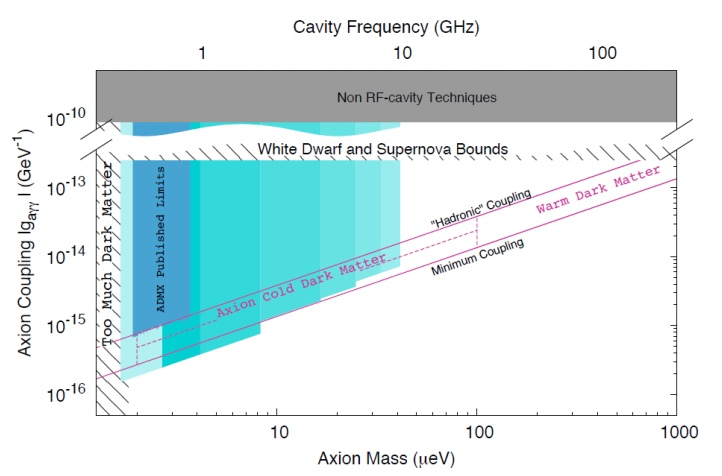
\includegraphics[width=0.95\textwidth]{admx2_limits}
	\caption{The projected sensitivity of the ADMX Generation 2 axion search (shaded regions).  Note that strong cosmological constraints are placed on the mass range and the axion coupling is also constrained by the mass.  The ADMX collaboration predicts that the searches shown will be completed by 2022 \cite{stern2016admx}.}
\end{figure}

\subsection{WIMPs}


Weakly interacting massive particles (WIMPs), which will be the focus of the remainder of this work, have proven to be the most popular dark matter candidate historically.   WIMPs not only satisfy the basic criteria listed at the beginning of this section but additionally they have what is referred to as the ``WIMP Miracle" in their favor.  In the early stages of the universe, the temperature and density were so large that all particles were in a state of chemical equilibrium.  A dark matter particle could annihilate by colliding with its anti-partner to form any type of particle and vice versa.  As time passed, however, the universe expanded and cooled making it more unlikely for these dark matter particles to be created or destroyed.  Using this thermal equilibrium model alongside the $\Lambda$CDM model, one can infer that the CDM density in the universe today is approximately given by \cite{jungman1996supersymmetric, bertone2010particle}

\begin{equation}
        \Omega_{CDM}h^2 \approx \frac{3 \times 10^{-27} \mathrm{cm}^3  \mathrm{s}^{-1}}{\left< \sigma_{ann} v \right> }
\end{equation}

where $\left< \sigma_{ann} v \right>$ is thermally averaged annihilation cross-section of cold dark matter.  Incredibly enough, if we assume that cold dark matter has properties such as cross-section and mass on the weak scale, we find that $\Omega_{CDM}h^2 \approx 0.1$, which is in agreement with cosmological constraints. 

In addition to WIMPs agreeing with cosmological evidence, several WIMP-like particles having masses on the order of 100 GeV with very long lifetimes naturally fall out of extensions of the standard model, such as supersymmetry.  



\section{Detecting WIMPs}

\begin{figure}[b]
	\centering
	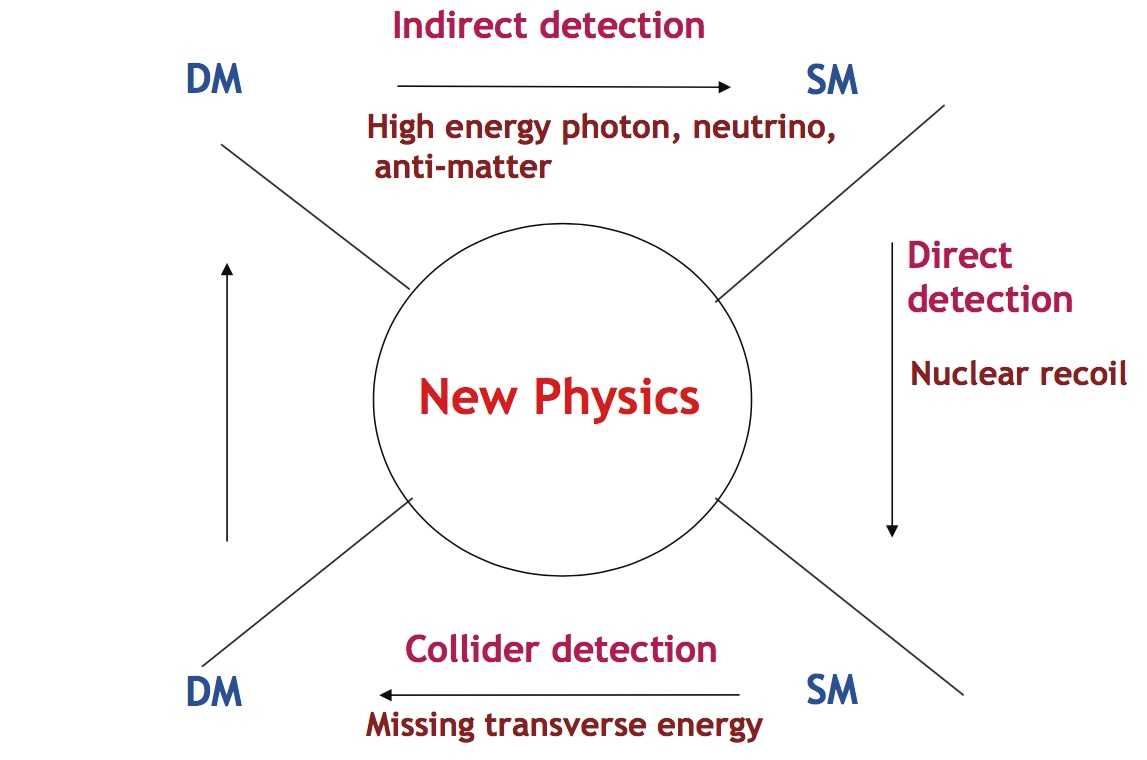
\includegraphics[width=0.75\textwidth]{wimp_detection}
	\caption{The three general approaches to WIMP detection: indirect detection, collider detection, and direct detection.  Image Credit: \cite{bi2013status}.}
	\label{fig:wimp_detection}
\end{figure}

Over the last few decades there has been an enormous concerted effort to detect WIMPs.  This effort has been focused in three general approaches: indirect detection, collider detection, and direct detection.  \figref{fig:wimp_detection} shows the idea behind these approaches:

\begin{itemize}
        \item Indirect detection looks for the annihilation of WIMPs in our galaxy into ordinary matter
        \item Collider detection is an attempt at creating WIMPs by colliding ordinary matter
        \item Direct detection looks for the scattering of WIMPs with ordinary matter
\end{itemize}

In this section we will discuss these three detection approaches with an emphasis on direct detection.  We will conclude with a brief discussion of the current direct detection experiments and notable results from this sector.

\subsection{Indirect Detection}
\label{sec:indirect_detection}
%https://arxiv.org/pdf/1404.1938.pdf

As we know from previous sections, WIMPs, if they make up all (or some) of the dark matter in the universe, must reside in galaxies to explain the odd behavior of rotation curves and the mass discrepancies.  Given the observational evidence, simulations have been created that can predict both the distribution of dark matter within our own and other galaxies \cite{stadel2009quantifying, maccio2007concentration} and the density of dark matter in our own solar system (roughly $0.2 - 0.4 \, \frac{\textrm{GeV}}{\textrm{cm}^3}$ \cite{read2014local}).  Indirect detection experiments look at high density regions of dark matter halos, such as in or around the Milky Way center and dwarf galaxies, to search for annihilations of WIMPs into detectable particles.

The goal of indirect detection is to capture a dark matter annihilation by observing its byproducts.  In the ideal case, two dark matter particles would annihilate and create two photons with energies equal to the mass of the dark matter particle.  Even though this would be the ``smoking gun" evidence of dark matter, most of the standard model extension WIMPs predict that this would be highly suppressed.  Instead, these indirect experiments are more likely to observe the annihilation of WIMPs into other particles which in turn will produce photons \cite{bi2013status}.  

A major difficulty in indirect detection experiments is distinguishing potential signals from normal astrophysical processes.  Since areas of high dark matter density are also typically areas of high astrophysical activity it becomes difficult to separate potential dark matter signals from potentially new astrophysics \cite{zitzer2015search}.  However, in recent years, astrophysicists have started turning their telescopes towards dwarf galaxies, which are dark matter dominated but have negligible astrophysical backgrounds \cite{conrad2014indirect}.  %For example, in 2012 the Fermi Large Area Telescope (Fermi-LAT) observed a line at 130 GeV near the galatic center in excess of the expected background with a significance of 4.5 sigma \cite{tempel2012fermi}.  However, over the last few years, this line has largely been ruled out by other experiments \cite{abdalla2016hess}



\subsection{Collider Detection}

The main idea behind collider detection is that since the WIMP is expected to have a mass on the order of $1-10^3$ GeV we can create it in particle accelerators.  Of course, detectors at particle accelerators are not designed to detect dark matter directly so when searching for WIMPs physicists must actually search for missing transverse energy (MET) in a collision.  The MET can be reconstructed by observing the outgoing particles and jets in a collision based on momentum conservation.  This reconstruction is shown in \figref{fig:collider_detection}.  Ultimately, this MET can be used to determine the mass and the new physics processes of the WIMP \cite{bi2013status}.

\begin{figure}[b]
	\centering
	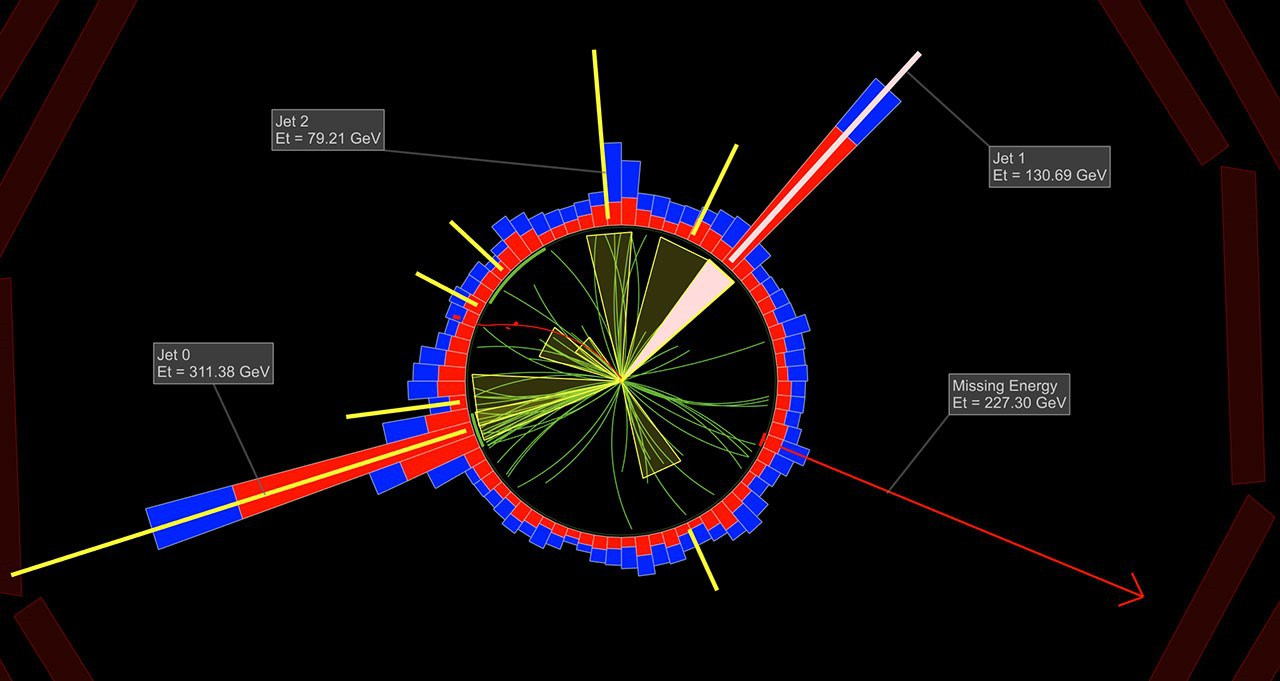
\includegraphics[width=0.95\textwidth]{collider_detection_cms}
	\caption{An image of a potential WIMP event in the CMS detector at CERN.  If a WIMP is present in a collision, momentum would not be conserved after all jets and particles have been accounted for in the collision.  Here we can see that after the three jets are reconstructed that there is still a large MET that could potentially be attributed to a WIMP.  Image Credit: Matevz Tadel, UC San Diego/CMS.}
	\label{fig:collider_detection}
\end{figure}

One important note is that while we can potentially ``see" WIMPs in detectors at colliders,  it is impossible to be certain that this WIMP is what makes up the majority of the matter in the universe.  The same signal would need to be seen in indirect and direct searches as well to make such a confirmation \cite{queiroz2016dark}.


\subsection{Direct Detection}

In purely theoretical terms, any detector that is sensitive to a potential WIMP interaction could be considered a direct detection dark matter search.  At the same time, to try and detect a dark matter signal from a NaI detector in your lab would be preposterous (unless your detector is 250 kg and located deep underground!), the reason being that any of the rare dark matter signals would be drowned out by the countless background events you would also detect.  This is why direct detection experiments are typically built deep underground with shielding and low radiation materials and take great care to understand their background as well as they possibly can: if WIMPs are scattering in the detector they want to be able to know.

The goal of direct detection experiments is to detect the scattering of WIMPs off of standard model particles.  As mentioned, since these scatters should be extremely rare, it is essential to have the background of the detector used be as low as possible.  As a simple example, consider two otherwise identical experiments who both have measured their backgrounds perfectly: experiment A expects a single background event per year while experiment B expects 1,000 background events per year.  In the case that both detectors see an excess of ten events in a given year over their background, it should be clear that experiment A can make a very strong claim that they have seen WIMP scatterings whereas experiment B cannot since this excess could very well be a fluctuation from their expected background.

It cannot be emphasized strongly enough how crucial the understanding of background is for direct detection experiments.  Returning to the above example, imagine experiment A missed a source of background in their estimate and that their true expected background rate is ten events per year, not one.  If they saw the same eleven events as before, they might claim a discovery even though the eleven events are very likely to be a statistical fluctuation of the background.


The most basic models describing WIMPs predict that they are most likely to interact with atomic nuclei (although some predict leptonic interactions \cite{kopp2009dama}).  This assumption, along with cosmological evidence that WIMPs are non-relativistic, surprisingly gives way to a fairly straight-forward derivation of the rate of scattering that one could expect for different nuclei, and therefore a complete detector, assuming a given scattering cross-section and mass for the WIMP.  For a complete derivation one should refer to \citeref{jungman1996supersymmetric} and \citeref{lewin1996review}.

It can be shown that the differential scattering rate is given by \cite{undagoitia2015dark}
%
\begin{equation}
        \frac{dR}{dE}(E) = \frac{\rho_0}{m_{\chi} m_{A}} \int_{v_{\textrm{min}}(E)}^{v_{\textrm{esc}}} v f(v) \frac{d\sigma}{dE}(E, v) dv
\end{equation} 
%
where $\rho_0$ is the local dark matter density, $m_{\chi}$ is the mass of the WIMP, $m_{A}$ is the mass of the target nucleus, $f(v)$ is the velocity distribution of dark matter locally, $v_{min}$ is the minimum velocity that can produce a recoil of energy $E$, $v_{esc}$ is the maximum velocity in which WIMPs are still gravitationally bound to the galactic halo, and $\frac{d\sigma}{dE}$ is the differential cross-section of WIMP-nucleon scattering.  

As discussed in \secref{sec:indirect_detection}, N-body simulations give us a prediction of roughly $0.2 - 0.4 \, \frac{\textrm{GeV}}{\textrm{cm}^3}$ for the local dark matter density \cite{read2014local}.  We will use the standard halo model (SHM), which is standard for dark matter experiments,  such that the velocity of WIMPs in the halo follows a Maxwell-Boltzmann distribution.  The minimum velocity of a WIMP to transfer an energy $E$ to a nucleus, $v_{min}$, is found kinematically to be 
%
\begin{equation}
        v_{min} = \sqrt{\frac{m_A E}{2 \mu^2}},  \quad
        \mu = \frac{m_A m_{\chi}}{m_A + m_{\chi}}
\end{equation}
%
while astrophysical measurements of the Milky Way estimate the local escape velocity to be $v_{esc} = 533^{+54}_{-41} \, \textrm{km} \, \textrm{s}^{-1}$ \cite{piffl2014rave}.  It is worth noting that while the Maxwell-Boltzmann distribution is the standard, other models of the velocity distribution exist \cite{kuhlen2010dark}.

The particle physics of the WIMPs comes in at the differential cross-section.  The most basic WIMP models predict two potential interactions: a spin-independent or spin-dependent.  Focusing on the former, the differential cross-section is given by
%
\begin{equation}
        \frac{d \sigma}{dE}(E, v) = \frac{m_A}{2 \mu^2 v^2} \sigma_0 F(E)^2
\end{equation}
%
where $F(E)$ is nuclear form factor.  The nuclear form factor is the Fourier transform of the ground state mass density and is used to correct the zero-momentum transfer cross-section in the case of a momentum transfer.  The nuclear form factor can be approximated by
%
\begin{equation}
        F(q) = \frac{3 j_1(q R_0)}{q R_0} e^{\frac{-(qs)^2}{2}}, \quad q=\sqrt{2 m_A E}, \quad R_0^2 = \left( 1.2A^{\frac{1}{3}} \, \textrm{fm} \right)^{2} - 5s^2
\end{equation}
%
where $q$ is the momentum transfer in the scatter, $R_0$ is the approximate nuclear radius, $s$ is the approximate thickness of the nucleus (roughly 1 fm), and $j_1$ is the spherical Bessel function of the first kind \cite{engel1991nuclear}.  

We can reduce $\sigma_0$, the cross-section of an interaction with zero momentum transfer, by accounting for the coupling to the individual nucleons in the following way
%
\begin{equation}
        \sigma_0 = \frac{\left( Z f_p + (A-Z)f_n \right)^2}{f_p^2} \frac{\mu^2}{\mu^2_{\chi p}} \sigma_p
\end{equation}
%
In this equation, $f_p$ and $f_n$ are the WIMP couplings to the proton and neutron, respectively, $\mu_{\chi p}$ is the reduced mass of the WIMP-proton system, and $\sigma_p$ is the spin-independent cross-section of the WIMP with the proton.  We approximate that $f_p \approx f_n$ which allows us to simplify to

\begin{equation}
        \sigma_0 \approx A^2 \frac{\mu^2}{\mu^2_{\chi p}} \sigma_p
\end{equation}

All of this can be combined such that we are only dependent on two variables: the mass of the WIMP and its cross-section with a proton.

\begin{equation}
        \frac{dR}{dE} = \frac{\rho_0 A^2 \sigma_p}{2 m_{\chi} \mu_{\chi p}^2} F(E)^2 \int_{v_{\textrm{min}}(E)}^{v_{\textrm{esc}}}  \frac{f(v)}{v} dv
\end{equation}

With the differential scattering rate, we can predict the number of WIMPs of a given cross-section and mass we would expect to scatter in a detector wth a certain target mass, M, in a given time period, T.  Notice that, as expected, the larger your detector is and the longer you run, the more likely you are to see a WIMP.

\begin{equation}
        N(\sigma_p, m_{\chi}) = M \, T \int \frac{dR}{dE} dE
\end{equation}



The differential scattering rates for a few targets and for different WIMP masses can be seen in \figref{fig:wimp_scattering_rate}.  Notice that xenon, with its very large nucleus, gives a significantly higher scattering rate versus most other targets for a wide range of energies.  Also notice that as the mass of the WIMP decreases, the differential scattering rate curve becomes steeper and steeper meaning that low mass WIMPs become increasingly difficult to observe.

% image of scattering rate for different nuclei and scattering rate for different WIMP masses in Xe
\begin{figure}[t]
	\centering
	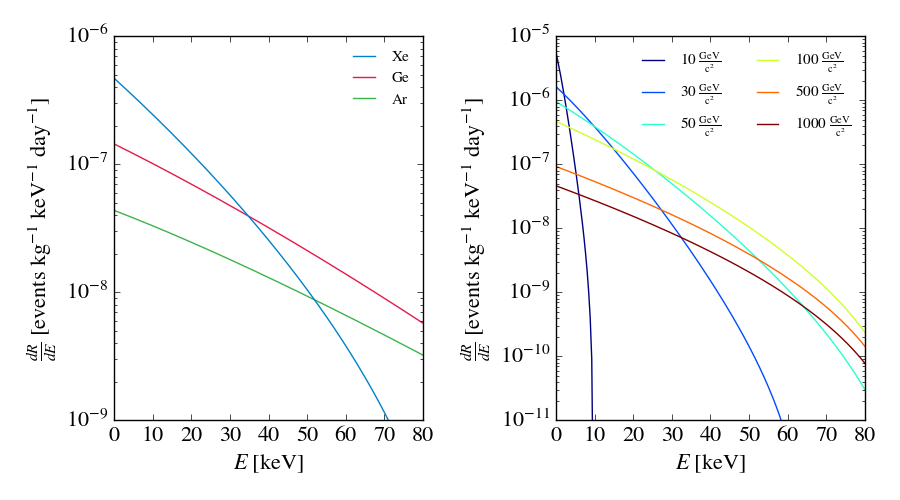
\includegraphics[width=0.99\textwidth]{wimp_recoil_rates}
	\caption{On the left are the differential scattering rates for a 100 $\sfrac{\textrm{GeV}}{\textrm{c}^2}$ WIMP with a spin independent cross section of $10^{-47} \, \textrm{cm}^2$.  On the right are the differential recoil spectra for WIMPs scattering with a xenon nuclei with a spin independent cross section of $10^{-47} \, \textrm{cm}^2$ assuming different WIMP masses.}
	\label{fig:wimp_scattering_rate}
\end{figure}


\subsection{Direct Detection Experiments}

The field of direct detection experiments is likely best described as diverse.  A WIMP interacting in a detector can deposit energy resulting in heat, ionization, or scintillation.  Current direct detection experiments leverage all three of these possibilities and many use two of these channels simultaneously to better discriminate types of interactions (electronic vs. nuclear recoils).  

\begin{figure}[t]
	\centering
	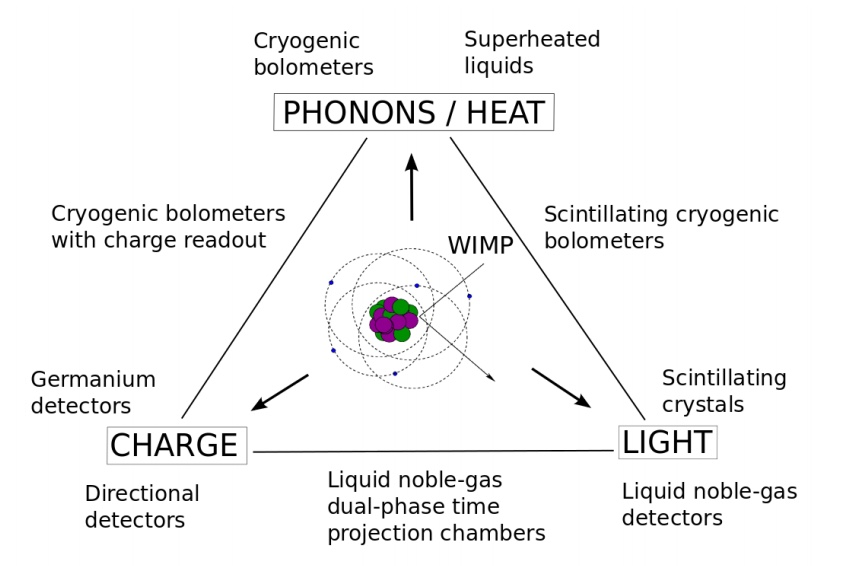
\includegraphics[width=0.99\textwidth]{dm_expts_2}
	\caption{A diagram showing the possible observables and observable combinations along with the most common detector types for each.  Image courtesy: \cite{undagoitia2015dark}.}
	\label{fig:dm_expts}
\end{figure}

\subsubsection{Heat}

There are two basic strategies of measuring the heat deposit of potential WIMP interactions that are on opposite sides of the temperature spectrum: cryogenic thermometers and super-heated liquids (bubble chambers).  Cryogenic thermometers are detectors cooled down to mK levels that measure the energy deposited by an interaction via the increase in temperature.  In recent years, these cryogenic thermometers have been coupled with light and charge detectors in order to discriminate between electronic and nuclear recoils to some extent \cite{strauss2016exploring}.  

Bubble chambers operate by filling a detector with a super-heated liquid that is just below its boiling point.  When ionizing radiation enters, it will form bubbles that can be detected by acoustic sensors.  One major advantage of bubble chambers is that they are almost completely insensitive to radiation that interacts electronically which is the main source of background for almost all other experiments.  The PICO collaboration uses bubble chamber technology to search for dark matter and they currently have the most stringent spin-dependent dark matter limits \cite{amole2017dark}.  

\subsubsection{Scintillation}

Scintillators have proven to be some of the most useful detectors in all of physics.  The operating principle is that as radiation pass through a detector, it excites the atoms and molecules in the medium which in turn produce light.  In single-channel scintillation experiments, scintillating inorganic crystals, such as NaI, are typically used.  Inorganic crystals are typically doped with an additional element, most commonly thallium, to increase their light yield and alter the wavelength to one that is more sensitive to photomultiplier tubes (the devices that are used to convert the light into an electrical signal).  The major downside of using an inorganic crystal, however, is that one cannot discriminate between different types of recoils in the detector \cite{undagoitia2015dark}.  The most famous experiment to use an inorganic crystal is the DAMA collaboration, which utilized a 250 kg NaI(Tl) crystal.  Since their operation began they have seen a statistically significant annual modulation in their event rate that agrees with predictions of how a dark matter signal would vary over the course of the year according to the standard halo model \cite{bernabei2010particle}.   \figref{fig:dama_modulation} shows this annual modulation.  However, the claim that the signal is dark matter has been extremely controversial since other experiments have been unable to replicate the results under the assumptions of many models and even an annual modulation test in an alternate detector \cite{aalseth2014maximum, xmass2016direct, aprile2017search}.

\begin{figure}[t]
	\centering
	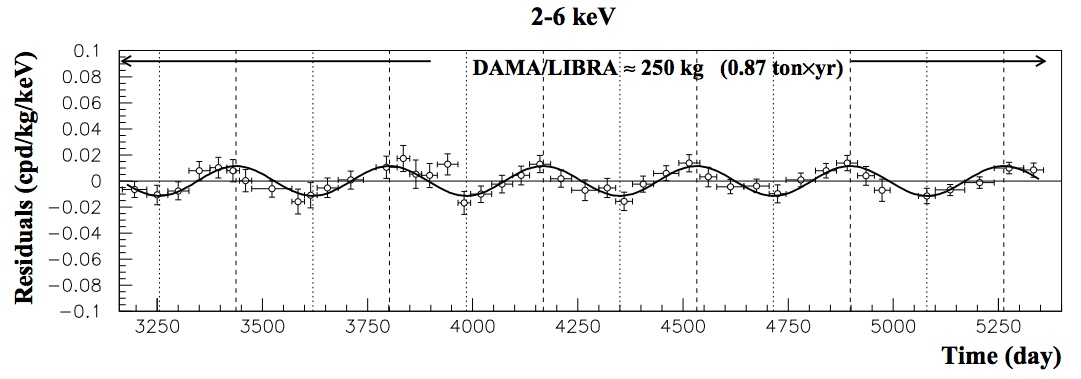
\includegraphics[width=0.99\textwidth]{dama_modulation}
	\caption{The annual modulation seen by the DAMA collaboration.  The modulation is statistically significant yet is in contrast to other experiments who fail to see the same signal. Image Credit: \cite{undagoitia2015dark}.}
	\label{fig:dama_modulation}
\end{figure}

While many experiments use condensed noble gasses that scintillate, they typically measure both scintillation and ionization in the medium.  However, there are some experiments that are hoping to witness a WIMP interaction while only measuring scintillation.  XMASS-I, for example, is a detector with an 832 kg liquid xenon target that, like DAMA, employed an annual modulation approach in their search for WIMPs.  Unlike DAMA, however, they see no annual modulation in their data \cite{xmass2016direct}.  

A useful property of condensed noble gasses is that there are usually two states in which the atoms or molecules can be excited into, a singlet and triplet state each with different decay times, and different types of interaction (electronic versus nuclear) will produce each in different fractions.  For argon, this difference in lifetime between the states is from less than 6 ns to 1,300 ns \cite{heindl2011table} meaning that pulse shape discrimination (PSD) is possible, while for xenon the difference is only 4.3 ns to 22 ns meaning that PSD is very difficult.  DEAP-3600, a 3600 kg liquid argon detector, uses this pulse shape discrimination technique to identify nuclear recoils in their detector \cite{amaudruz2017first}.     


\subsubsection{Ionization}

The majority of experiments that used charge as their only channel utilized high-purity germanium detectors.  These type of detectors operate by having incoming particles free electrons in a consistent and linear fashion as function of energy.  These types of detectors are able to observe interactions at much lower energies than most other detectors, allowing them to probe lower WIMP masses.  The most recent of these single-channel HPGe experiments was CoGeNT.  In early 2014, CoGeNT announced that they also had seen an annual modulation that matched the standard halo model \cite{aalseth2014search} however this was found to be an error in the estimation of the background \cite{aalseth2014maximum}.


\subsubsection{Heat-Scintillation}

As mentioned earliers, many of the experiments that use heat as a channel also couple it with another channel.  CRESST-II is an example of such an experiment --- CREST-II uses a roughly 5 kg target of $\textrm{CaWO}_4$ that is cooled to mK temperatures.  The detector also utilizes a small silicon-on-sapphire absorber to measure the scintillation light produced.  The addition of this scintillation detector enables the detector to discriminate between electronic recoil background and potential nuclear recoil signals \cite{strauss2016exploring}.  

\subsubsection{Heat-Ionization}

The HPGe crystals used to detect ionization signals can also be cooled such that measuring heat signals is possible.  One example of this procedure is in the EDELWEISS-III experiment.  In EDELWEISS-III, 24 800 g HPGe detectors cooled to 18 mK were employed in their search for WIMPs. Again, this combination of channels allows EDELWEISS-III to discriminate electronic from nuclear recoils in their detector \cite{armengaud2016constraints}.

\subsubsection{Scintillation-Ionization}

While many of the experiments mentioned excel at low mass, none have been as successful as dual-channel scintillation-ionization experiments above masses of approximately 5 GeV.  Specifically, dual-phase liquid xenon time projection chambers (TPCs) have led the field in the WIMP search from roughly 5 GeV to 1 TeV for almost a decade.  As of this writing, XENON1T, the first ton-scale dual-phase TPC, holds the strongest limit of spin-independent WIMP scattering, as can be seen in \figref{fig:dm_si_limits} \cite{aprile2017first, collaboration2017dark}.  Not only are these detectors capable of a high level discrimination between electronic and nuclear recoils but they are also capable of measuring the position of an interaction in the detector allowing further elimination of background sources.  However, one of the major difficulties of these types of experiments is that the response of liquid xenon to low energy electronic and nuclear recoils is not well understood.  A great deal of effort has gone into measuring the response of xenon to these low energy interactions and later we will focus on an experiment designed for exactly this purpose.

\begin{figure}[t]
	\centering
	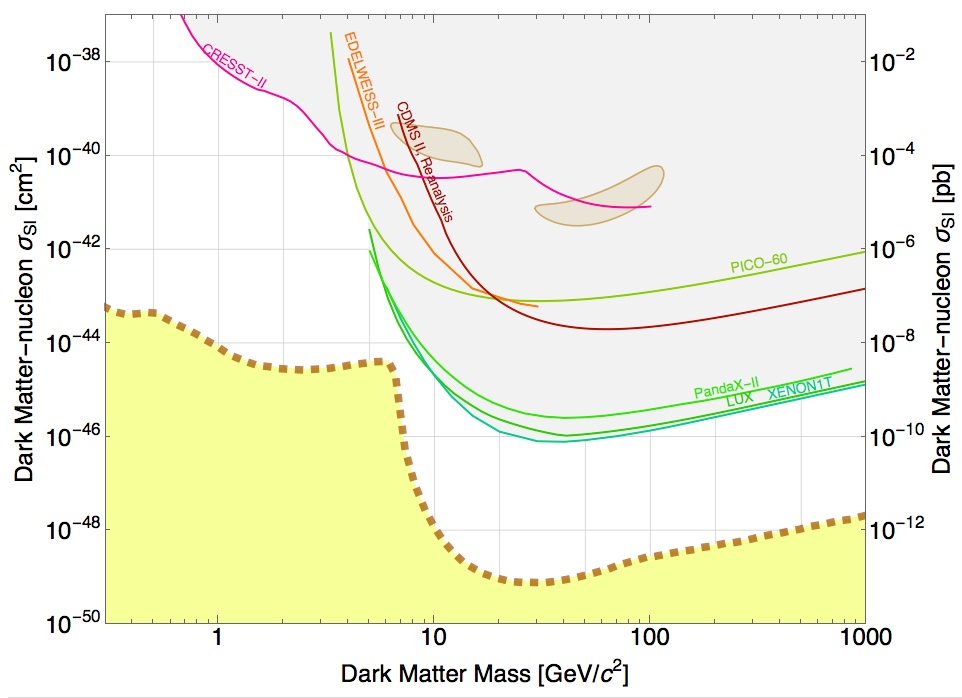
\includegraphics[width=0.99\textwidth]{dm_si_limits}
	\caption{Selected spin-independent WIMP limits from selected experiments and the discovery contour from DAMA's annual modulation.  The dashed line shown in brown marks the point where neutrinos will become a background source in WIMP searches.  Notice that the three liquid xenon dual-phase TPC based experiments (PandaX-II, LUX, and XENON1T) set the strongest limit over a wide range of WIMP masses \cite{agnese2015improved, armengaud2016constraints, savage2009compatibility, amole2017dark, tan2016dark, akerib2017results, aprile2017first, angloher2016results, ruppin2014complementarity}.}
	\label{fig:dm_si_limits}
\end{figure}





%This is the second chapter of the dissertation

%The following command starts your chapter. If you want different titles used in your ToC and at the top of the page throughout the chapter, you can specify those values here. Since Columbia doesn't want extra information in the headers and footers, the "Top of Page Title" value won't actually appear.

\pagestyle{cu}
\graphicspath{{./Chapter2/images/}}

\chapter[Liquid Xenon and Dual-Phase TPCs][Liquid Xenon and Dual-Phase TPCs]{Liquid Xenon and Dual-Phase TPCs}
\label{chap:lxe}

This chapter will focus on liquid xenon as a detector medium.  In \secref{sec:lxe_chem_properties} we will discuss the general properties of liquid xenon along with some of the benefits and considerations of these properties.  In \secref{sec:energy_deposition} we will discuss how charged particles in xenon deposit their energy.  In \secref{sec:lxe_er} we will discuss the production of observable light and charge from electron recoils while in \secref{sec:lxe_nr} we will discuss observable production from elastic nuclear recoils.  Finally, in \secref{sec:lxe_tpc}, we will discuss how these observables are detected in dual-phase xenon time projection chambers.

\section{General Properties}
\label{sec:lxe_chem_properties}

Xenon, with an atomic number of 54, is a noble gas meaning that it has a full valence electron shell.  Because of the full valence shell, xenon is very unlikely to interact chemically with other elements and molecules.  Xenon is also the heaviest noble gas that is, for practical purposes, naturally non-radioactive.  \ce{^{136}Xe}, with a natural abundance of 8.857\%, has been show to undergo double beta decay with a half-life of $2.165 \cdot 10^{21}$ years so strictly speaking natural xenon is radioactive although this process is extremely rare and has little relevance for even low background dark matter experiments \cite{albert2014improved}.

While natural xenon is not radioactive, it is actually possible to excite xenon nuclei such that they decay and emit gamma rays.  None of these excited states have very long lifetimes that would cause issues for low background experiments but two of these neutron activated states (\ce{^{131m}Xe} and \ce{^{129m}Xe} which decay emitting 164 keV and 236 keV photons, respectively) have half-lives on the order of ten days.  This half-life could potentially be very useful in the calibration of large detectors since over this period of time the excited states would be approximately uniformly distributed inside of a detector \cite{ni2007preparation}.

Xenon is extracted from the atmosphere as a byproduct of the separation of oxygen and nitrogen.  Once the oxygen is separated, it will contain trace amounts of krypton and xenon that can be separated out further by distillation or adsorption.  The xenon that is purchased commercially typically will have a final Kr/Xe ratio of $\sim 10^{-6} - 10^{-9} \frac{\textrm{mol}}{\textrm{mol}}$.  Natural krypton is not radioactive on a relevant time scale but \ce{^{85}Kr}, which is released into the atmosphere via nuclear fuel reprocessing and nuclear weapons tests, beta decays with a mean energy of 251 keV and with a half-life of roughly 10.8 years \cite{abe2009distillation}.  So while natural xenon is not radioactive, the process of extracting xenon from the atmosphere does leave a radioactive isotope that could be a potential source of background for dark matter experiments.  Significant effort has gone into reducing the Kr/Xe levels to reduce this background as much as possible.  In XENON1T, the lowest level to date was achieved with a natural krypton to xenon ratio of less than 200 ppq (1 ppq = $10^{-15} \frac{\textrm{mol}}{\textrm{mol}}$) \cite{aprile2017removing}.



\begin{table}[t]
\centering
\label{tab:xe_abundance}
\def\arraystretch{1.3}
\begin{tabular}{ccccc}
\hline
Isotope & Abundance & Spin & Half-life & Decay Mode  \\ \hline
\ce{^{124}Xe} & 0.095\% & 0 & $ > 1.6 \cdot 10^{14}$ y & $2 \nu \beta^+ \beta^+$ \cref{fn:predicted_decay} \\ %\hline
\ce{^{126}Xe}&  0.089\% & 0 & $ 4.7 - 12 \cdot 10^{25}$ y & $2 \nu \beta^- \beta^-$ \cref{fn:predicted_decay} \\ %\hline
\ce{^{128}Xe}&  1.910\% & 0 & Stable & - \\ %\hline
\ce{^{129}Xe}&  16.400\% & $\sfrac{1}{2}$ & Stable & - \\ %\hline
\ce{^{130}Xe}&  4.071\% & 0 & Stable & - \\ %\hline
\ce{^{131}Xe}&  21.232\% & $\sfrac{3}{2}$ & Stable & - \\ %\hline
\ce{^{132}Xe}&  26.909\% & 0 & Stable & - \\ %\hline
\ce{^{134}Xe} & 10.436\% & 0 & $ > 5.8 \cdot 10^{22}$ y & $2 \nu \beta^- \beta^-$ \cref{fn:predicted_decay} \\ %\hline
\ce{^{136}Xe}&  8.857\% & 0 & $2.2 \cdot 10^{21}$ y & $2 \nu \beta^- \beta^-$ \\ %\hline
\end{tabular}
\caption{Abundances, half-lives, and decay modes of various xenon isotopes.  Note that \ce{^{136}Xe} is the only isotope whose decay has been measured.  Half-life data: \cite{barros2014double}.}
\end{table}
\stepcounter{footnote}



Dual-phase xenon experiments typically operate at roughly 2--3 atm, which translates to a boiling point of roughly 180 K ($-93.2^{\circ}$ C).  The density of liquid xenon (LXe) at this temperature is roughly 2.84 $\sfrac{\textrm{g}}{\textrm{cm}^3}$ which is significantly higher than all of the other noble elements, with the exception of radon \cite{rankin2009crc}.  The high density of LXe is partly responsible for its high electronic stopping power, which will be discussed further in the next section.

\begin{figure}[t]
	\centering
	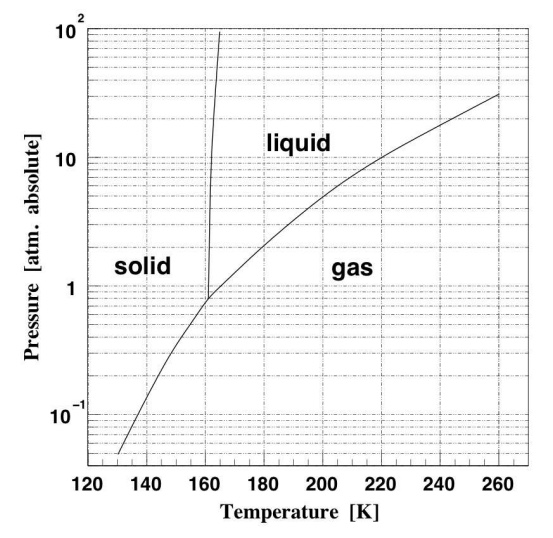
\includegraphics[width=0.7\textwidth]{xe_pt_diagram}
	\caption{The phase diagram for xenon.  Dual-phase xenon TPCs typically operate in the range of 2--3 atm.}
	\label{fig:xe_phase_diagram}
\end{figure}



\section{Energy Deposition of Charged Particles in Liquid Xenon}
\label{sec:energy_deposition}

Both nuclear and electronic recoils, which will be discussed in the following sections, ultimately result in a charged particles traversing the LXe - in the case of an electronic recoil the resulting charged particle is an electron and in the case of nuclear recoils it is the xenon nucleus.  Given the high density and atomic number of xenon, the electronic stopping power is large for both electrons and xenon ions ($\sim 1-30 \, \sfrac{\textrm{keV}}{\mu \textrm{m}}$).  This means that the tracks of low energy electronic and nuclear recoils will be very small and approximately point-like \cite{aprile2006simultaneous}.

In liquid xenon (and other noble liquids), scintillation light is produced via the excitation of atomic electrons and the ionization and subsequent recombination of free electrons and ions.  The excitation scintillation process is shown in \eqnref{eqn:exciton_production} and the ionization scintillation process is shown in \eqnref{eqn:ionization_production}.  


% foot note for table
\footnotetext{\label{fn:predicted_decay}This decay is predicted but has not yet been observed.}

\begin{equation}
        \label{eqn:exciton_production}
        \begin{gathered}
                \textrm{Xe*} + \textrm{Xe} + \textrm{Xe} \rightarrow \textrm{Xe*}_2 + \textrm{Xe}, \\
                \textrm{Xe*}_2 \rightarrow 2\textrm{Xe} + h \nu
        \end{gathered}
\end{equation}


\begin{equation}
        \label{eqn:ionization_production}
        \begin{gathered}
                \textrm{Xe}^+ + \textrm{Xe} \rightarrow \textrm{Xe}_2^+, \\
                \textrm{Xe}_2^+ + e^- \rightarrow \textrm{Xe**} + \textrm{Xe}, \\
                \textrm{Xe**} \rightarrow \textrm{Xe*} + \textrm{heat}, \\
                \textrm{Xe*} + \textrm{Xe} + \textrm{Xe} \rightarrow \textrm{Xe*}_2 + \textrm{Xe}, \\
                \textrm{Xe*}_2 \rightarrow 2\textrm{Xe} + h \nu
        \end{gathered}
\end{equation}

The excitation process proceeds when an an atomic electron in xenon is excited (the excited xenon is referred to as an \textit{exciton}) and the excited atom forms a dimer with another xenon atom, which is called an \textit{excimer}.  This excited excimer can be formed in either the singlet state (spin of excited electron anti-parallel to electron originally sharing state) or triplet state (spin of excited electron parallel to electron originally sharing state).  The excimers in the singlet and triplet states each have their own characteristic lifetimes (roughly 4 ns and 22 ns)\footnote{In xenon the difference in lifetimes of the singlet and triplet states is fairly small but for argon the singlet lifetime is 7 ns while the triplet lifetime is 1.3 $\mu$s \cite{heindl2011table}!} and decay into xenon atoms and a 178 nm photon (the photon falls in UV portion of the spectrum) \cite{hitachi1983effect, doke2002absolute}.  

The ionization process begins when a charged particle ionizes a xenon atom, leaving singly-ionized xenon and a free electron.  The singly-ionized xenon atom can then form an ionized dimer and subsequent excited xenon state.  This excited xenon state leads to an excimer through non-radiative heat loss.  The excimer produces scintillation light in the manner described above.

% mention charge signal
Implicit in the ionization process outlined above is the assumption that the electron freed during ionization recombines with the singly-ionized dimer.  However, in the presence of an electric field, this recombination can be reduced such that a charge signal can also be read out in addition to the scintillation signal.  Incomplete recombination can also occur at zero electric field and these electrons are called \textit{escape electrons} (although you cannot extract the charge signal without an applied electric field) \cite{doke2002absolute}.


\begin{figure}[t]
	\centering
	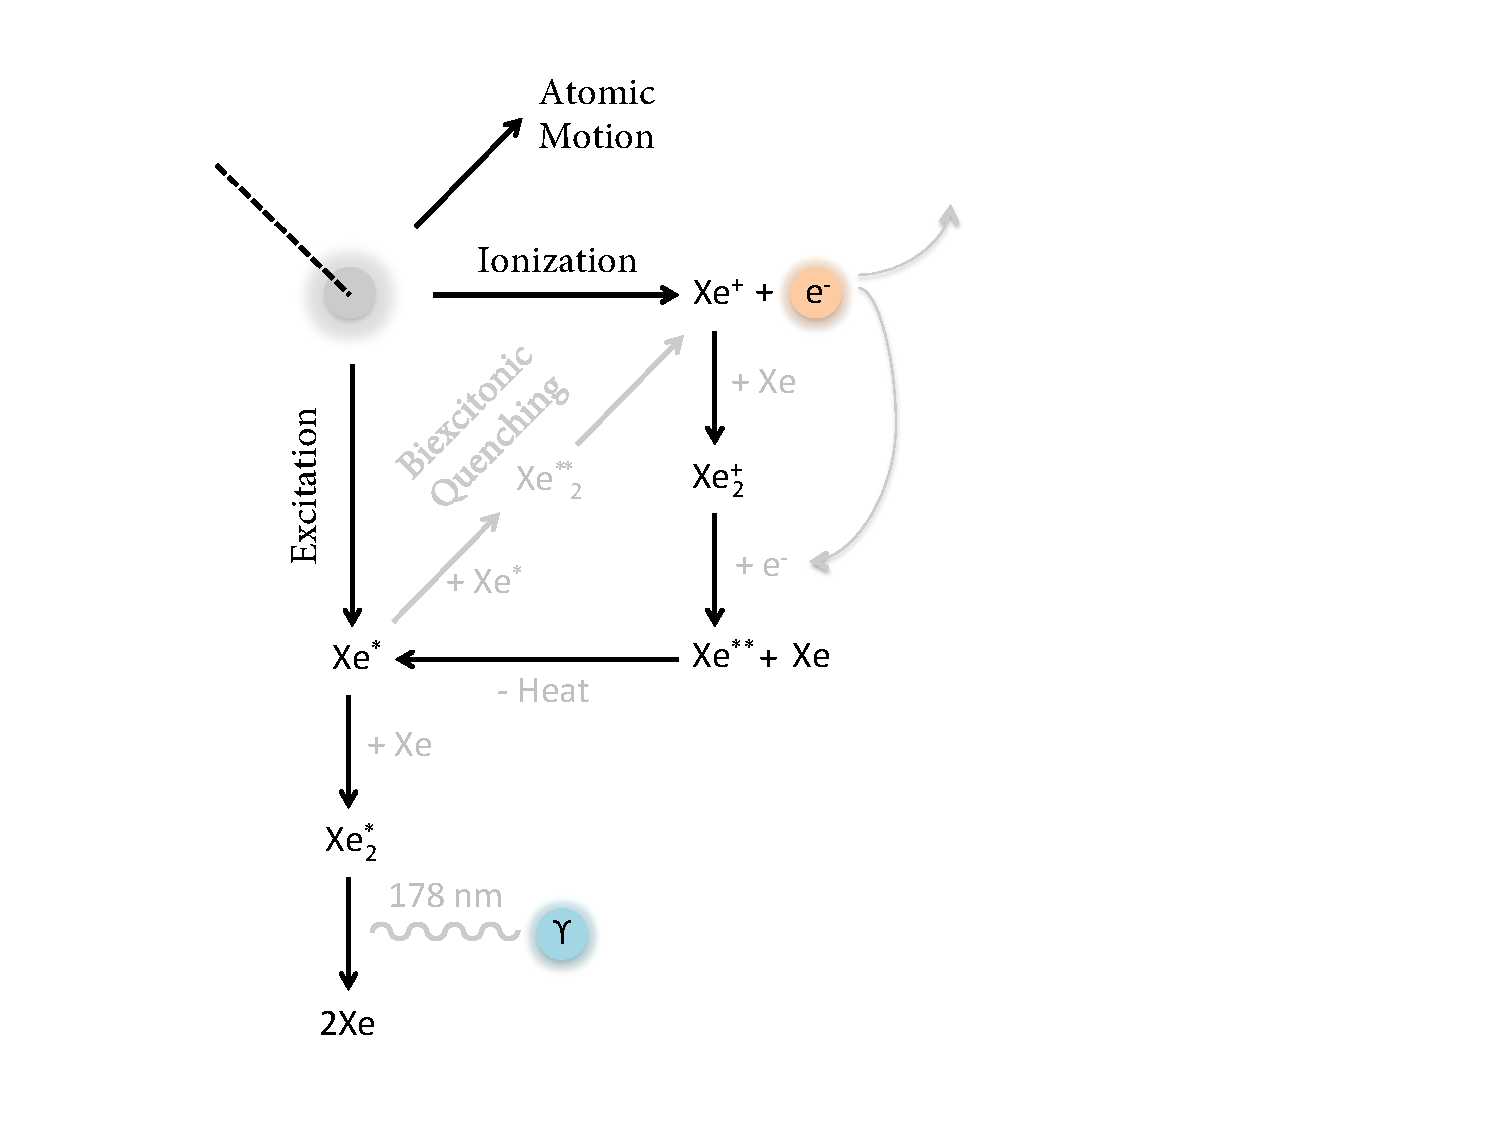
\includegraphics[width=0.7\textwidth]{observables_diagram}
	\caption{A diagram showing the modes in which charged particles may lose energy in liquid xenon.  Note that when an electric field is applied, the electron freed during ionization can be extracted such that it can be measured.}
	\label{fig:diagram_energy_deposition}
\end{figure}

% important to note xenon ions lose energy via heat too...
% pg 4 of Lindhard paper
It is important to note that while these electronic excitation and ionization mechanisms are dominant for electronic recoils, the energy deposition for nuclear recoils is split between these and atomic motion.  This distinction is extremely important - the energy given to electrons in a recoil cannot cause atomic motion however atomic motion, if sufficiently slow, will not be able to cause excitation or ionization in other atoms and hence some energy is lost.  This effect was first discussed by Lindhard in 1963 \cite{lindhard1963integral} and the effort to quantify this effect continues today and in this work.  This effect will henceforth be referred to as nuclear quenching.

A second form of quenching has been observed in high linear energy transfer (LET) interactions, specifically with $\alpha$ scatters in xenon (which will not be discussed in detail) and high energy nuclear recoils.  This quenching is called biexcitonic quenching and is the result of two excitons colliding to produce an electron-ion pair as shown in \eqnref{eqn:biexcitonic_quenching}.

\begin{equation}
        \label{eqn:biexcitonic_quenching} 
        \textrm{Xe*} + \textrm{Xe*} \rightarrow \textrm{Xe} + \textrm{Xe}^+ + e^-
\end{equation}

Since this form of electronic quenching requires the collision of two excitons, it is expected that the track density ultimately determines the level of quenching \cite{hitachi2005properties}.

A diagram showing all of the mentioned energy deposition methods for charged particles is shown in \figref{fig:diagram_energy_deposition}.



\section{Electronic Recoils in Liquid Xenon}
\label{sec:lxe_er}

In this section, we will discuss the sources of electronic recoils in liquid xenon, their properties, and how they result in detectable observables.  For dual-phase LXe TPCs (which we will focus on in more detail later) searching for ``standard'' WIMPs, electronic recoils constitute the background.  With a precise understanding of what causes electronic recoils and how they interact in LXe, we can better discriminate between electronic recoils and potential signals that are expected to interact via nuclear recoils.  Additionally, if WIMPs do interact with atomic electrons rather than the nucleus, a precise understanding of the electronic recoil background would be crucial for a discovery.  

\subsection{Sources of Electronic Recoils}

There are two main sources of energetic electrons in liquid xenon: (1) beta decays from contaminants inside of a detector and (2) photons interacting through matter via photoelectric absorption, Compton scattering, or pair production.  In either case, the resulting energetic electron creates a track through the xenon, mainly losing its energy from inelastic collisions with atomic electrons.   In standard WIMP hypotheses, WIMPs are expected to interact with the atomic nucleus, however there are certain theories of WIMPs that allow interactions between a WIMP and atomic electrons that would result in an electronic recoil. 

\subsubsection{Beta Decays}

While there are both $\beta^-$ and $\beta^+$ decays, we will focus on $\beta^-$ decays since they are relevant to WIMP searches.  $\beta^-$ decay is a radioactive decay in which a neutron is converted to a proton inside of the nucleus and a subsequent electron and anti-electron neutrino are emitted.  This type of decay is made possible by the weak force which allows a quark to change its type via a W boson and an electron and anti-neutrino (positron and neutrino) pair \cite{cottingham1987introduction}.

While the maximum energy of the energetic electron in the decay is fixed, because an anti-neutrino is also emitted in $\beta^-$ decay, the energy spectra of the electron is continuous.  This continuous energy spectrum is what makes long-lived $\beta^-$ emitters very dangerous potential sources of background - they can, with non-negligible probabilities, produce electrons with energies of interest for WIMP detection ($\lesssim 15$ keV).  The energy spectrum for \krypton{} is shown in \figref{fig:kr85_beta_decay}.

\begin{figure}[t]
	\centering
	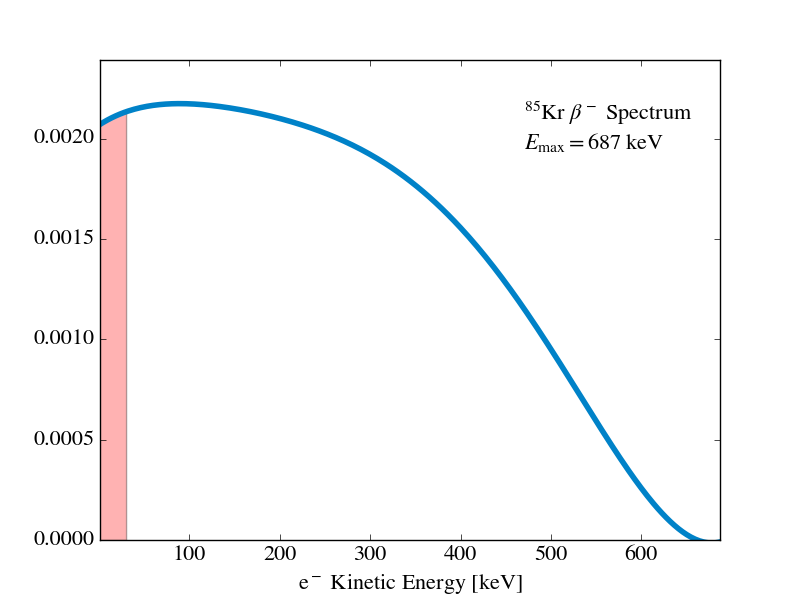
\includegraphics[width=0.7\textwidth]{kr85_beta_rates}
	\caption{The kinetic energy spectrum of electrons resulting from the $\beta^-$ decay of \ce{^{85}Kr} \cite{mantel1972beta}.  Note that roughly 3.1\% of decays are below 15 keV (shaded red region) which puts them inside the energy region of interest of WIMP searches.}
	\label{fig:kr85_beta_decay}
\end{figure}

% show multiple energy spectra of the beta decays from 
%https://ac.els-cdn.com/0020708X7290107X/1-s2.0-0020708X7290107X-main.pdf?_tid=259893f2-a843-11e7-9dfb-00000aacb35f&acdnat=1507039388_aef3096471a4defbd8b1c8a8198864c6

In liquid xenon based detectors, the two biggest sources of background beta decays are from \ce{^{85}Kr} and \ce{^{214}Pb}, which comes from the \ce{^{222}Rn} decay chain \cite{aprile2017first}.  Even though certain atoms that $\beta^-$ decay prove to be a background that must be carefully reduced, others have proven to be extremely useful for detector calibrations.  \ce{^{212}Pb}, from the decay chain of \ce{^{220}Rn},  has proven useful for calibrations since approximately 10\% of electrons have an energy less than 15 keV (the maximum energy is 570 keV) \cite{aprile2017radon}.  Perhaps even more exciting for the low energy calibrations of electronic recoils is the use of tritium, which has a maximum energy of only 18.6 keV \cite{akerib2016tritium, aprile2017tritium}! \footnote{Molecular tritium ($\textrm{T}_2$) cannot be used because it adsorbs to surfaces very easily and the half-life of $\textrm{T}_2$ is 12.3 years.  Instead, tritiated methane ($\textrm{CH}_3\textrm{T}$) is used since this will not adsorb and can be easily removed.}  

\subsubsection{Photons}

Another source of electronic recoils in LXe comes from photons.  Photons, via photoelectric absorption, Compton scattering, or pair production, can create energetic electrons inside of a detector.  While pair production is not relevant in the energy range of interest, photoelectric absorption is one of the most tried and tested calibration tools for LXe (and other detectors) and electrons from Compton scatters can make up part of the background in WIMP searches since the energy of the electron can be arbitrarily low.

Photoelectric absorption is the process by which a photon is absorbed by an atom from which an electron is subsequently ejected (typically from the K shell).  This implies that the energy of the ejected electron is equal to the energy of the photon minus the binding energy.  However, the newly ionized atom will have a free electron bind with it, usually on a very short time scale, and an X-ray or auger electron will be emitted \cite{knoll2010radiation}.  Therefore the energy detected from photoelectric absorption will be very close to the initial energy of the photon.  Photoelectric absorption is the dominant mode of interaction up to a few hundred keV in most media, including xenon as can be seen in \figref{fig:photon_attenuation}.  

\begin{figure}[t]
	\centering
	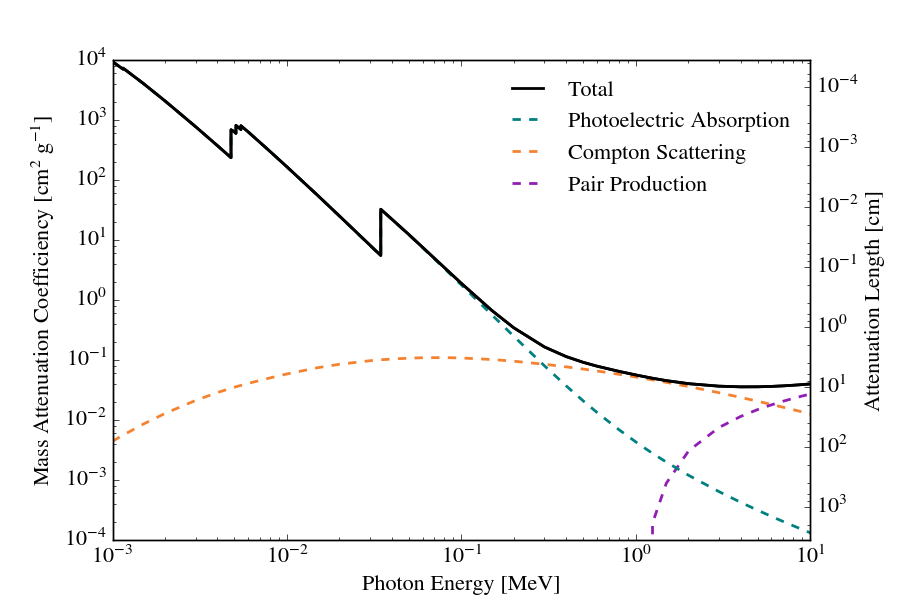
\includegraphics[width=0.95\textwidth]{photon_attenuation}
	\caption{The mass attenuation coefficient and the attenuation lengths for photons of different energies in liquid xenon \cite{berger8coll}.}
	\label{fig:photon_attenuation}
\end{figure}

Compton scattering is the process by which a photon interacts with an atomic electron resulting in the deflection of the photon at a specific angle and a transfer of energy to the electron.  The angle of the scattering completely describes the energy transferred to the electron.  Compton scattering is the dominant mode of interaction from a few hundred keV to a few MeV in most media, including xenon as can be seen in \figref{fig:photon_attenuation}.

\figref{fig:photon_attenuation} shows the mass attenuation coefficient of photons in LXe and the individual contributions of each process.  Because of xenon's high atomic number, all processes have very high attenuation coefficients.  This is valuable for background reduction since low energy photons are absorbed at the very edge of the detector (since their attenuation length is $<$ 1 cm) although it does make calibration with external gamma ray sources very difficult for large detectors.\footnote{This is the reason why many large scale LXe detectors are calibrated using internal sources now such as the beta emitters mentioned earlier and metastable activated xenon.}  Photons with an energy of a few hundred keV to a few MeV are most likely to Compton scatter and not be absorbed and have an attenuation length on the order of several centimeters which means that they will contribute to the background of LXe detectors at some level.
 

\subsubsection{Neutrons}

Neutrons can interact in liquid xenon mainly through three mechanisms: radiative absorption and inelastic scattering, which result in electronic interaction in the medium, and elastic scattering, which ultimately results in a nuclear recoil and will be discussed in \secref{sec:lxe_nr}.   The cross-sections of each of these mechanisms for xenon can be seen in \figref{fig:neutron_cross_section}.  Note that for almost all energies between 1 keV -- 10 MeV that elastic scattering is the dominant process.


\begin{figure}[t]
	\centering
	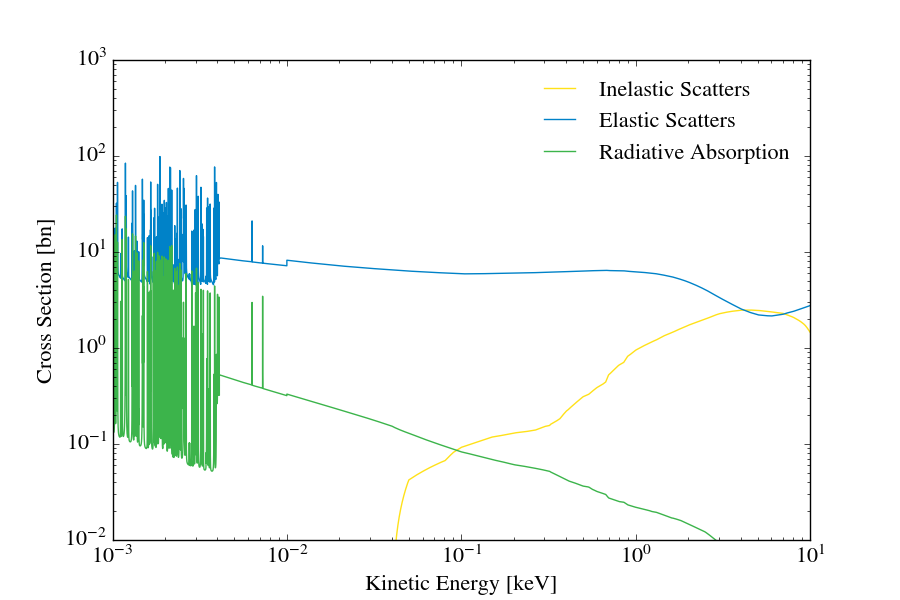
\includegraphics[width=0.95\textwidth]{neutron_cross_sections}
	\caption{The cross-sections of the three main interaction modes of neutrons in liquid xenon.  Note that elastic scattering is the dominant process for almost all energies in the range shown.  The data for each isotope of xenon is from \citeref{chadwick2011endf} and the figure shows the cross-sections weighted by abundance of each isotope in natural xenon.}
	\label{fig:neutron_cross_section}
\end{figure}


Radiative absorption is the absorption of neutrons by a nucleus.  The nucleus thus increases by one in mass number with atomic number staying the same.  Fortunately, since the isotopes of xenon that could be produced are not radioactive, with the exception of \ce{^{133}Xe} and \ce{^{135}Xe}, this process produces very little background.  \ce{^{133}Xe} and \ce{^{135}Xe} both result in short $\beta^-$ chains and will therefore result in electronic recoils inside of a detector.  With this said, for the neutron energies of background and calibrations in liquid xenon WIMP detectors, radiative absorption is largely irrelevant.

Inelastic scattering is the process by which a particle interacts with the atomic nucleus and kinetic energy is lost due to the excitation of the nucleus.  The excitation of the nucleus, also called \textit{activation}, is then followed by the nucleus decaying from this excited state back down to a stable state through the emission of a particle.  For xenon, there are two inelastic collisions of note:  an inelastic scattering with \ce{^{129}Xe} or \ce{^{131}Xe}.  A neutron scattering inelastically with \ce{^{129}Xe} can result in nucleus being in an excited state with a 0.96 ns half-life that decays into gamma ray at an energy of approximately 40 keV or in an excited metastable state with a half-life of 8.8 days that results in a 197 keV photon followed by a 40 keV photon (the 40 keV photon is from the same very short lived state that the metastable state decays into) \cite{timar2014nuclear}.  A neutron scattering inelastically with \ce{^{131}Xe} can result in the nucleus being in a metastable state with a half-life of 11.84 days that decays emitting a 164 keV photon \cite{khazov2006nuclear}.   While these processes are not relevant for background considerations during a WIMP search, they are very useful when calibrating a detector since they each result in electronic recoils at a low and fixed energy.

There are three major sources of neutrons in dark matter experiments.  The first major source is from heavy elements in various detector components decaying via spontaneous fission resulting in neutrons with energies typically from 1 -- 10 MeV.  Neutrons also come from high-energy muons interacting with the rock and materials around the detector.  Finally, neutrons can be produced artificially using a neutron generator (typically either through a deuterium-deuterium reaction or deuterium-tritium reaction).  The first two sources of neutrons make up background in dark matter searches while the third source of neutrons is used to calibrate detectors (for both electronic and nuclear recoils).


\subsubsection{Neutrinos}

% https://arxiv.org/pdf/1512.07501.pdf
% largest source of neutrinos is the sun

Neutrinos can elastically scatter with electrons either via charged-current (exchange of W boson) or neutral-current (exchange of Z boson) interactions.  For electronic recoils, the main sources of neutrinos are from initial deuterium production and \ce{^7Be} reactions inside the sun (roughly 92\% and 7\% of the neutrino background, respectively) \cite{aprile2016physics}.  Like electronic recoils from beta decays, the kinetic energy of the recoiling electron will follow a spectrum where only very low energies ($\lesssim 15$ keV) are relevant.  Unlike other sources of electronic recoils, the solar neutrino background cannot be reduced.

% example recoil spectrum shown in: https://journals.aps.org/rmp/pdf/10.1103/RevModPhys.59.505

%franarin2016reducing
\begin{figure}[t]
	\centering
	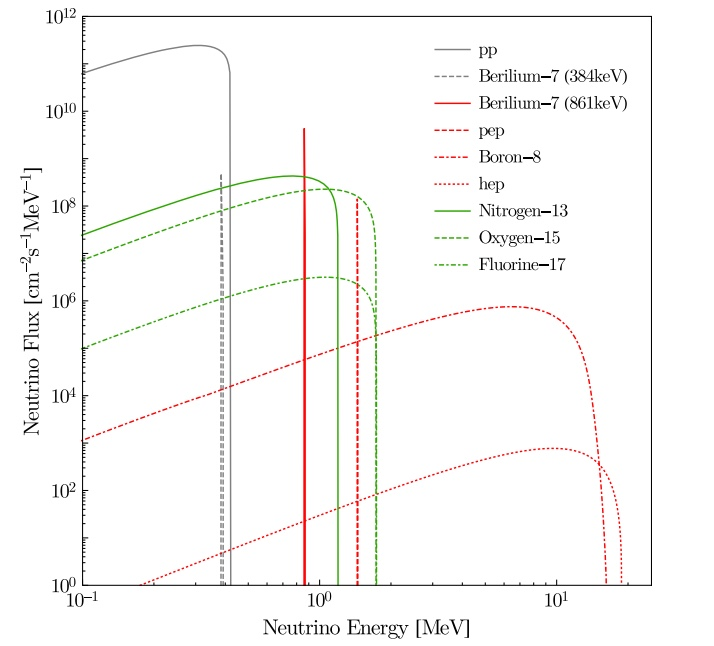
\includegraphics[width=0.7\textwidth]{solar_neutrino_flux}
	\caption{Solar neutrino fluxes from different processes assuming the BS05(OP) standard solar model.  Image Credit: \cite{franarin2016reducing}.}
	\label{fig:solar_neutrino_flux}
\end{figure}

\subsection{Observables Production for Electronic Recoils}
\label{sec:lxe_er_observables}

In \secref{sec:energy_deposition}, we discussed the modes by which charged particles deposit energy in LXe.  We will now quantify these observables production methods for electronic recoils under the assumption of an applied electric field.

As mentioned in \secref{sec:energy_deposition}, electronic recoils result in either excitation or the creation of electron-ion pairs.  Assuming the recoils occur in the presence of an electric field, we do not need to be concerned about quenching with respect to escape electrons (since these can be extracted by the electric field and ultimately measured).  Additionally, electronic recoils have relatively sparse tracks (as can be seen by their low stopping power in liquid xenon) \cite{aprile2006simultaneous} so it is expected that biexcitonic quenching will not play a large role in observables production.

Since there are no major forms of quenching, we can completely separate the energy deposited in the electronic recoil into excitons and electron-ion pairs.  Typically the total number of quanta (excitons and electron-ion pairs) is used to describe this relationship --- specifically, the average energy required to produce a single quanta.  For xenon, this value is $W = 13.7 \pm 0.2 \, \textrm{eV}$ \cite{dahl_thesis} and the relationship is given by \eqnref{eqn:w_value}.

\begin{equation}
        \label{eqn:w_value}
        N_q = \frac{\textrm{E}_{\textrm{ER}}}{W} = N_{\textrm{ex}} + N_{\textrm{ion}}
\end{equation}  

This relationship, while looking very simple, turns out to be extremely useful for calibrations in dual-phase xenon TPCs, as we will discuss in later chapters.  The breakdown of excitons to electron-ion pairs is simply described by the ratio of the two quantities such that we can define probabilities of a given quanta being an exciton or electron-ion pair.

\begin{equation}
        p_{\textrm{ion}} = \frac{1}{1 + \frac{N_{\textrm{ex}}}{N_{\textrm{ion}}}}, \, \, \, p_{\textrm{ex}} = 1 - p_{\textrm{ion}}
\end{equation}

The exciton-to-ion ratio, $\frac{N_{\textrm{ex}}}{N_{\textrm{ion}}}$, has been theoretically calculated to be 0.06 for sub-MeV electronic recoils \cite{takahashi1975average} however measurements and theoretical predictions have also suggested a value of $0.20 \pm 0.13$ \cite{doke2002absolute, aprile2007observation}.   

As mentioned previously, electron-ion pairs have a finite probability of recombining to form excitons and eventually producing a scintillation signal (as opposed to a charge signal).  While in the past this recombination probability was modelled using Birks' saturation law \cite{birks2013theory} for large tracks and the Thomas-Imel model \cite{thomas1987recombination} (which will be discussed in more detail for nuclear recoils) for short tracks, recently a great deal of work has gone into directly measuring recombination in liquid xenon and its potential fluctuations without the assumption of a model \cite{akerib2016tritium, aprile2017tritium}.  Recombination is simply inserted to the model of observables production as shown in \eqnref{eqn:recombination_er}.

\begin{equation}
        \label{eqn:recombination_er}
        N_{\textrm{ex}} \leftarrow N_{\textrm{ex}} + r N_{\textrm{ion}}, \, \, \, N_{\textrm{ion}} \leftarrow (1 - r) N_{\textrm{ion}}
\end{equation}

Following recombination in electronic recoils, these excitons and electron-ion pairs directly translate into the number of photons and electrons that are observable.

\begin{equation}
        \label{eqn:er_observables}
        N_{\gamma} = N_{ex}, \, \, \, N_e = N_{ion}
\end{equation}

\section{Nuclear Recoils in Liquid Xenon}
\label{sec:lxe_nr}

It is expected that WIMPs could potentially dissipate energy in xenon via elastic nuclear recoils so understanding these type of interactions is of crucial importance for WIMP direct detection experiments.  In this section, we will discuss the sources of nuclear recoils in liquid xenon based WIMP searches (besides potential WIMPs) and the observables production process for elastic nuclear recoils, which is substantially more complicated due to the nuclear and electronic quenching first mentioned in \secref{sec:energy_deposition}.

\subsection{Sources of Nuclear Recoils}

The two sources of nuclear recoils in liquid xenon based WIMP searches, besides potential WIMPs, are neutrons and neutrinos.   While neutrons are, as one would expect, the main background and calibration source in liquid xenon based WIMP searches, neutrinos are no longer negligible and, as detectors become more and more sensitive to lower cross-sections, will soon comprise an irreducible background of elastic nuclear recoils in detectors.  Understanding the sources of nuclear recoils in liquid xenon based WIMP direct detection experiments is very important since an underestimation of the background could lead to potential claims of a false WIMP signal since interactions would be indistinguishable on an event-by-event basis.

\subsubsection{Neutrons}

Electronic recoils from neutron scattering were discussed in \secref{sec:lxe_er} --- in this section we will focus on nuclear recoils from elastic scattering.  Elastic scattering is the process by which a particle interacts with the atomic nucleus and kinetic energy is conserved.  The recoiling nucleus then deposits its energy in the medium which can ultimately be detected.  Particles scattering elastically with nuclei is also called a nuclear recoil.  Of course, this process is not unique to neutrons but is the main mode of interaction for many massive particles (and hopefully WIMPs).  

Each of the sources of neutrons mentioned in \secref{sec:lxe_er}, spontaneous fission of heavy materials, high-energy muons, and artificially generated muons, can also result in nuclear recoils.




\subsubsection{Neutrinos}

Neutrinos can interact with both electrons, as discussed in \secref{sec:lxe_er}, and atomic nuclei, via coherent neutrino-nucleon scattering (CNNS).  The maximum energy of a recoiling nucleus is given by $E_{\textrm{r}}^{\textrm{max}} = \frac{2 E_{\nu}^2}{m_N + 2 E_{\nu}}$, where $m_N$ is the mass of the nucleus and $E_{\nu}$ is the energy of the neutrino.  This implies that neutrinos must have energies on the order of 10 MeV to cause nuclear recoils on the order of 1 keV.  Therefore, high energy neutrino sources like \ce{^{8}B} in the sun as well as neutrinos from supernovae and the atmosphere will contribute the most to the CNNS background in dark matter experiments.


\subsection{Observables Production for Nuclear Recoils}
\label{sec:xe_nr_observables}

We will now discuss the details of the observables production process for nuclear recoils that was generally outlined in \secref{sec:energy_deposition}.  Like electronic recoils, nuclear recoils can lead to the excitation or ionization of other xenon atoms.  However, unlike energetic electrons in liquid xenon, recoiling xenon atoms will also interact with other xenon nuclei.  This distinction is extremely important since energy can effectively be ``lost'' if the energy transferred during a collision is too low to cause excitation or ionization.  

Lindhard proposed a theory to describe this nuclear queching in \citeref{lindhard1963integral}.  To describe the quenching of signals due to atomic motion, it is standard to work with the dimensionless energy given in \eqnref{eqn:dimensionless_energy}.

\begin{equation}
        \label{eqn:dimensionless_energy}
        \epsilon = 11.5 \left( \frac{E}{\textrm{keV}} \right) Z^{\sfrac{-7}{3}}
\end{equation}

Lindhard showed that at low velocities ($v < v_F$) the stopping power of a heavy ion in a medium is approximately given $S_e = k \epsilon^{\sfrac{1}{2}}$, where $k$ is a proportionality constant, assuming the Thomas-Fermi screening model.  Under the same assumptions, it can be shown that $k = 0.133 Z^{\sfrac{2}{3}} A^{-\sfrac{1}{2}}$, which would give $k \approx 0.165$ for xenon, although in his original paper Lindhard names the calculation of the proportionality factor as the largest source of uncertainty in the stopping power.  Shown in \eqnref{eqn:lindhard_electronic} is Lindhard's semi-empirical numerical solution for the fraction of the total energy that goes to electronic interactions for recoiling atoms.

\begin{equation}
        \label{eqn:lindhard_electronic}
        L(\epsilon) = \frac{k g(\epsilon)}{1 + k g(\epsilon)}, \, \, \, g(\epsilon) = 3 \epsilon^{0.15} + 0.7 \epsilon^{0.6} + \epsilon
\end{equation}

Note that $g(\epsilon)$ is not derived from first principles but is a fit to Lindhard's numerical solution from $\epsilon = 0.001 - 100$ (roughly 1 keV -- 100 MeV nuclear recoils for xenon).

Similar to observables production in electronic recoils, we assume that all energy that goes towards electronic interactions is converted into excitons and ions by way of the W value as is shown in \eqnref{eqn:quanta_nr}.

\begin{equation}
        \label{eqn:quanta_nr}
        N_q = \frac{L(E) E_{\textrm{NR}}}{W} = N_{\textrm{ex}} + N_{\textrm{ion}}
\end{equation}

As with electronic recoils, the split into excitons and ions can be defined by a single parameter, $\frac{N_{\textrm{ex}}}{N_{\textrm{ion}}}$.

\begin{equation}
        p_{\textrm{ion}} = \frac{1}{1 + \frac{N_{\textrm{ex}}}{N_{\textrm{ion}}}}, \, \, \, p_{\textrm{ex}} = 1 - p_{\textrm{ion}}
\end{equation}

Unlike electronic recoils, however, it is expected that $\frac{N_{\textrm{ex}}}{N_{\textrm{ion}}} \approx 1$ for nuclear recoils \cite{angle2011search, sorensen2011nuclear, lenardo2015global}.

RIVAL (Recoiling Ions in Various Atomic Liquids) simulations show that nuclear recoils, unlike electronic recoils, lose the majority of their energy in a large number of secondary tracks and have a short track size relative to electronic recoils.  With short tracks and with applied electric fields we can use the Thomas-Imel recombination model to describe the recombination of electrons and ions into excitons shown in \eqnref{eqn:ionization_production} \cite{dahl_thesis}.   The Thomas-Imel box model \cite{thomas1987recombination} begins by using the modified diffusion equation presented by Jaffe \cite{jaffe1913theory} with the assumptions that Coulomb forces are negligible, due to the high coefficient of polarization for xenon.  Jaffe's model is described by \eqnref{eqn:jaffe_recomb}.

\begin{equation}
        \label{eqn:jaffe_recomb}
        \frac{\partial N_{\pm}}{\partial t} = \mp u_{\pm} \bm{E} \cdot \bm{\nabla} N_{\pm} + D_{\pm} \nabla^2 N_{\pm} - \alpha N_+ N_-
\end{equation}

In \eqnref{eqn:jaffe_recomb} $N_{\pm}$ are the ion and electron charge distributions, $u_{\pm}$ are the ion and electron mobilities, and $\alpha$ is the recombination constant.  Thomas and Imel improved upon this model by making appropriate approximations for liquid xenon and argon: the diffusion rate is very small and ion drift is much slower than electron drift (3 -- 5 orders of magnitude).  These simplifications lead to the set of equations \ref{eqn:ti_diffeq}.

\begin{equation}
        \label{eqn:ti_diffeq}
        \begin{gathered}
                \frac{\partial N_+}{\partial t} = - \alpha N_+ N_- \\
                \frac{\partial N_-}{\partial t} = u_- E \frac{\partial N_-}{\partial z} - \alpha N_+ N_-
        \end{gathered}
\end{equation}

Assuming that the electron-ion pairs are isolated, that the initial distribution of ions and electrons uniformly populates a box of dimension $a$, and that $N_{ion}$ electron-ion pairs initially fill the box, we can solve equations \ref{eqn:ti_diffeq} to find the probability of recombination.

\begin{equation}
        \label{eqn:ti_recomb}
        r = 1 - \frac{\textrm{ln}(1 + N_{ion} \sigma)}{N_{ion} \sigma}, \, \, \, \sigma = \frac{\alpha}{4 a^2 \mu_- E}
\end{equation}

We redefine the number of excitons and electron-ion pairs following recombination in the same way as with electronic recoils.

\begin{equation}
        N_{\textrm{ex}} \leftarrow N_{\textrm{ex}} + r N_{\textrm{ion}}, \, \, \, N_{\textrm{ion}} \leftarrow (1 - r) N_{\textrm{ion}}
\end{equation}

Since nuclear recoils result in smaller and more dense tracks, we must also account for biexcitonic quenching.  Biexcitonic quenching occurs by the process outlined in \eqnref{eqn:biexcitonic_quenching}: two excitons collide ultimately leading to the formation of a single electron-ion pair.  This process effectively reduces the two potential photons to a single observable photon.  This electronic quenching is typically parameterized using the quenching term from Birks' saturation law, as shown in \eqnref{eqn:birks_quenching}, since one would expect that the density of excitons in a track to be proportional to the electronic stopping power \cite{mei2008model, tretyak2010semi, bezrukov2011interplay}. 

\begin{equation}
        \label{eqn:birks_quenching}
        f_B = \frac{1}{1 + \eta \frac{dE}{dx}} = \frac{1}{1 + \eta k \epsilon^{\sfrac{-1}{2}}}
\end{equation}

This quenching ultimately reduces the number of photons that will be observable in a given interaction, as shown in \eqnref{eqn:nr_observables}.

\begin{equation}
        \label{eqn:nr_observables}
        N_{\gamma} = N_{ex} f_B, \, \, \, N_e = N_{ion}
\end{equation}


% use following for biexcitonic quenching:
% https://ac.els-cdn.com/S0927650505000964/1-s2.0-S0927650505000964-main.pdf?_tid=e866eaac-a918-11e7-974f-00000aab0f6b&acdnat=1507131190_5bd95affa2fae24418f54ce96721ae8a
% https://arxiv.org/pdf/0712.2470.pdf
% https://ac.els-cdn.com/S0927650511001289/1-s2.0-S0927650511001289-main.pdf?_tid=baf2e1c0-a922-11e7-a7e2-00000aacb35d&acdnat=1507135409_d72980a38a6fbe81c7b4585e9dae6c97


\section{Dual-Phase Time Projection Chambers}
\label{sec:lxe_tpc}

Having discussed how different types of particles deposit their energy in liquid xenon, we can now discuss dual-phase xenon time projection chambers (TPCs), the leading detector type in the search for WIMPs, and how they identify interaction types and reconstruct the position and energy of interactions in a TPC.



\subsection{Operating Principle}
\label{sec:tpc_operating_principle}

On an interaction-by-interaction basis, the goal of dual-phase xenon TPC is three-fold: determine the type of the interaction (nuclear or electronic recoil), determine the energy of the interaction, and determine the position of the interaction.  While we will discuss in more detail how each of these goals is achieved in a TPC, it is important to understand how the observables are extracted from the liquid xenon.  

For both nuclear and electronic recoils, an interaction in the liquid xenon with an applied electric field results in both photons and free electrons.  The number of photons are measured by using photomultipler tube (PMT) arrays at the top and bottom of the detector.  These PMTs convert the light signal into a proportional charge signal that can be read by a standard digitizer.  This prompt scintillation signal is referred to as the S1 of the interaction.  The electric field that is applied vertically in the detector is used to extract the free electrons from the interaction site and to the liquid-gas boundary in the detector.  An additional electric field is applied to extract the electrons from the liquid and to accelerate the electrons through the gas, exciting xenon atoms that lead to secondary scintillation photons in the process.  This process occurs at a time directly related to the depth of the interaction in the liquid.  This secondary scintillation process, which is proportional to the number of electrons extracted from the interaction site, is referred to as the S2 of the interaction.  This entire process is depicted in \figref{fig:tpc_principle} and will be discussed in significantly more detail throughout the remainder of this chapter.

\begin{figure}[t]
	\centering
	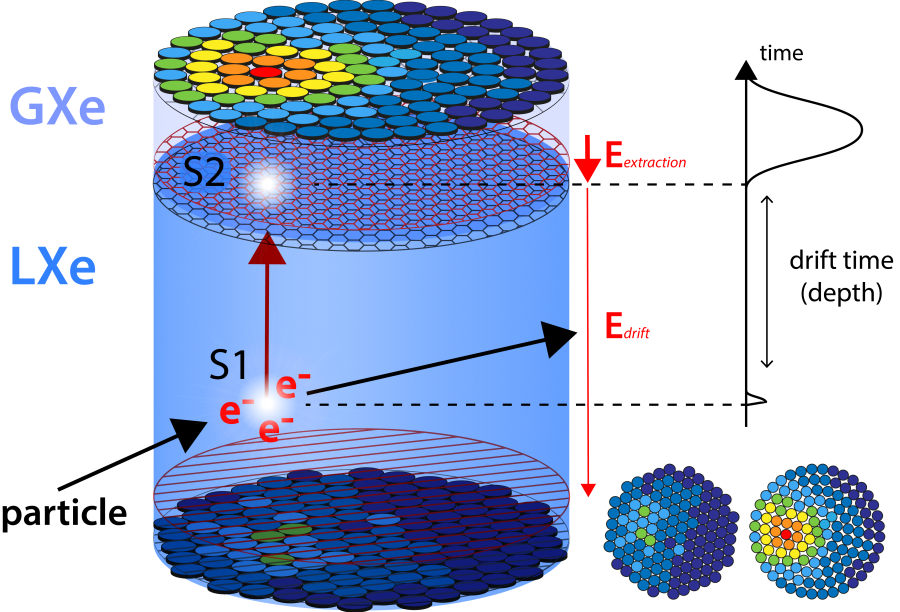
\includegraphics[width=0.99\textwidth]{tpc_principle}
	\caption{An example of an interaction in a dual-phase liquid xenon time projection chamber.  The interaction produces both scintillation light and free electrons.  The light is promptly detected by the PMT arrays at the top and bottom of the detector while the free electrons are drifted to the liquid-gas interface where they are extracted and accelerated through the gaseous xenon.  This acceleration through the gaseous xenon causes secondary excitations that result in more scintillation light that is detected by the PMT arrays.  The time difference between these interactions can be used to extract the depth of the interaction while the PMT hit patterns for the secondary signal can be used to find the interactions position in the transverse plane.}
	\label{fig:tpc_principle}
\end{figure}


\subsubsection{Reconstructing Interaction Type}

Since the most basic function of these TPCs is to search for WIMPs via elastic nuclear recoils, it becomes crucially important to be able say what is likely background (electronic recoils) and what is a potential signal (nuclear recoils).  Without this type of discrimination, searches are limited to counting techniques like those discussed in the first chapter.  Since the electronic recoil background rate is typically several orders of magnitudes larger than the nuclear recoil background, an experiment that can discriminate between the two interactions will be significantly more sensitive than a similar detector that is not.

As mentioned throughout this chapter, even though the energy deposition processes of electronic and nuclear recoils are similar they are far from identical.  These differences in track structure and interaction cross-sections lead to very large discrepancies in the amount of charge produced in an interaction relative to the amount of light produced at a given field.   For energies relevant to the WIMP search, the relationship shown in \eqnref{eqn:lxe_disc} holds for electronic and nuclear recoils and can be used to discriminate between them.  \figref{fig:xe1t_disc} shows this difference between electronic and nuclear recoils for XENON1T with a drift field of $116.7 \pm 7.5  \,\sfrac{\textrm{V}}{\textrm{cm}}$ \cite{aprile2017first}.

\begin{equation}
        \label{eqn:lxe_disc}
        \left( \frac{\textrm{S2}}{\textrm{S1}} \right)_{\textrm{ER}} > \left( \frac{\textrm{S2}}{\textrm{S1}} \right)_{\textrm{NR}}
\end{equation}

\begin{figure}[t]
	\centering
	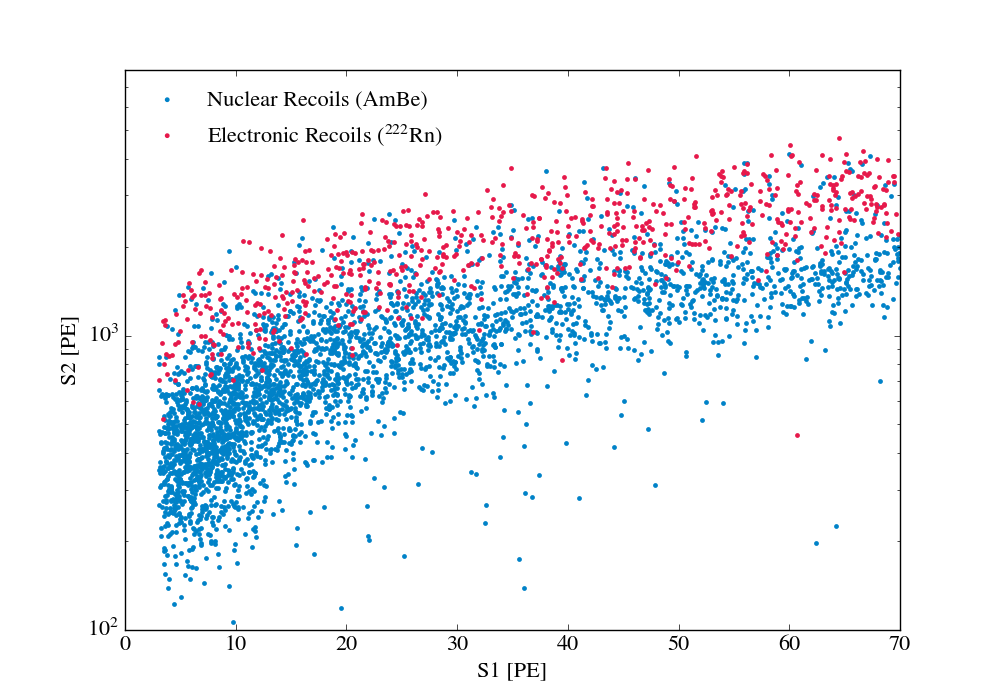
\includegraphics[width=0.99\textwidth]{xe1t_disc}
	\caption{Low energy electronic and nuclear recoils in liquid xenon.  Note that for a given S1 that the S2 for electronic recoils are usually significantly higher than the corresponding S2 for nuclear recoils.  The nuclear recoils are from an americium-beryllium (AmBe) source while the electronic recoils are from the \ce{^{222}Rn} decay chain that results in a $\beta^-$ emission with a maximum energy of 1.02 MeV.}
	\label{fig:xe1t_disc}
\end{figure}

This difference in the ratio of charge to light can actually be enhanced further: while $\frac{\textrm{S2}}{\textrm{S1}}$ for nuclear recoils has little to no dependence on the electric field applied in the TPC, $\frac{\textrm{S2}}{\textrm{S1}}$ for electronic recoils is heavily dependent on the electric field \cite{aprile2006simultaneous, goetzke2016measurement}, as can be seen in \figref{fig:field_dependence_nr_er}.  Therefore, the discrimination power between the two types of interactions can be increased by increasing the electric field used in the TPC.

\begin{figure}[t]
	\centering
	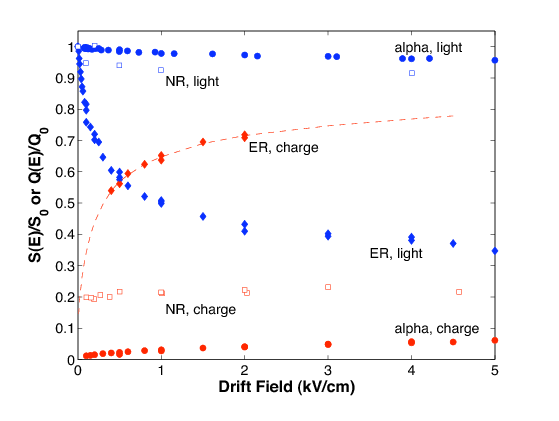
\includegraphics[width=0.85\textwidth]{field_dependence_nr_er}
	\caption{The field dependence of scintillation and ionization yield in liquid xenon for 122 keV electronic recoils and 56.5 keV nuclear recoils.  In blue are the light yields of interactions at a given field relative to the light yield with no applied electric field.  In red are the charge yields of interactions relative to the charge yield assuming no recombination.  Image Credit: \citeref{aprile2006simultaneous}}
	\label{fig:field_dependence_nr_er}
\end{figure}


\subsubsection{Reconstructing Energy}

A significant portion of this chapter was dedicated to understanding the production process of the observable photons and electrons in liquid xenon with an applied electric field.  With a perfect understanding of the observables production process and the detector effects, one could reconstruct the probability distribution for the energy of an event.  The reason you could not say the energy precisely, even with a perfect understanding of the physical processes described and the detector physics,  is because there is an associated smearing at each stage in the observables process -- in other words, two nuclear recoils depositing 10 keV at the same position in the detector will not produce exactly the same measured event each time.  

However, even being able to approximate the energy of an event is extremely important.  More precisely, an understanding of the process between energy deposition to the readout of observables is essential for the most sensitive dark matter searches.  The reason for this is because all predicted signals in the detector, including both background and potential WIMP signals, have a predictable energy spectrum.  Therefore, we can not only predict how many electronic and nuclear recoils there should be but we can also say \textit{where} they should be in an S1 and S2 spectrum.  As a concrete example, we expect the nuclear recoil background to fall off exponentially with increasing energy.  Therefore, an excess of events at high energies is more significant (or indicates a misunderstanding regarding the background) than an excess of events at low energies.


\subsubsection{Reconstructing Position}
\label{sec:xe_pos_rec}

An additional piece of information that proves to be very useful that can be extracted from TPCs is the the position of an event.  As mentioned earlier, an approximately uniform electric field is applied in the TPC to extract the electrons created in an interaction from the vertex to the liquid-gas interface where they will produce the secondary signal, the S2.  Of course, the scintillation light from the interaction is measured extremely quickly (on the order of nanoseconds such that we approximate the delay as zero) so the S1 can be used as the start of a timer that ends with the S2.  This drift time can then be used to reconstruct the depth of the interaction since the electron will travel with a constant velocity through the liquid xenon as given by $v_d = \mu E$, where $v_d$ is the drift velocity, $\mu$ is the mobility of electrons in liquid xenon, and $E$ is the electric field applied.   This analysis to determine the depth is shown on the right side of \figref{fig:tpc_principle}.

 \begin{figure}[t]
	\centering
	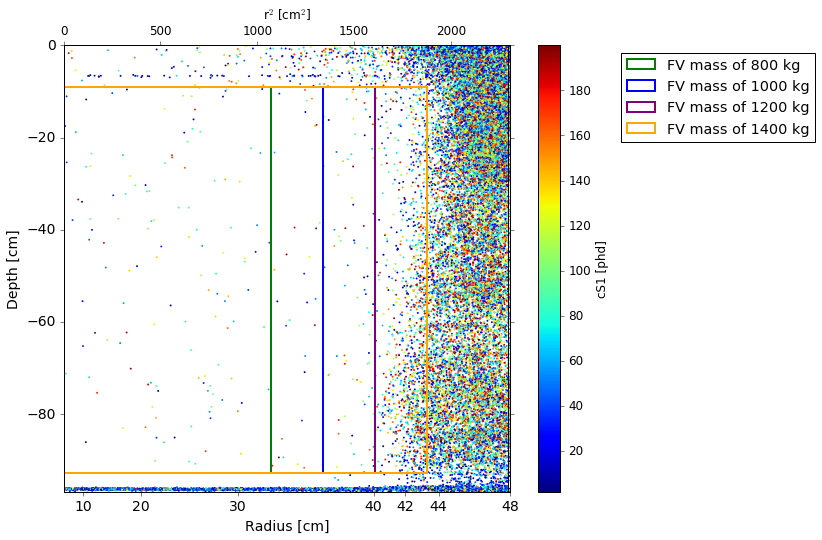
\includegraphics[width=0.99\textwidth]{tpc_pos_rec}
	\caption{The positions of all events during the first science run of XENON1T.  Notice that the overwhelming majority of events occur at the very edge of the detector and can be removed using a fiducial volume.}
	\label{fig:tpc_pos_rec}
\end{figure}

As mentioned earlier in this chapter, the stopping power for different charged particles in liquid xenon is high enough such that interactions will be stopped in $\lesssim 10 \, \mu \textrm{m}$.  Diffusion for electrons in liquid xenon is also small: even assuming a very large drift time of 1 ms, the expected transverse diffusion is on the order of $\sqrt{D_t t_d} \sim$ 20 mm so the electrons should still be very localized when arriving at the liquid-gas interface.  Once these electrons are accelerated through the gas layer they create the secondary photons (S2), which are then detected using the PMT arrays at the top and the bottom of the detector.  The hit pattern of the PMT arrays, specifically the top array, can be used to approximate the location of extraction at the liquid-gas interface, which should be a very good approximation of the position at the depth found using the drift time.  The PMT hit patterns are shown on the bottom-right of \figref{fig:tpc_principle}.

The three-dimensional location of an event inside a detector proves to be very important for WIMP searches.  To understand why, it is useful to consider a WIMP event in a detector.  Since the cross-section of the WIMP is so small, one would expect two features in a WIMP event: it would only scatter a single time and that it could scatter anywhere in the liquid xenon with equal probability.  However, this is very different from almost all of our external background sources (the exception, of course, being neutrinos) - both external gamma, beta, and neutron sources that emit particles into the liquid xenon are expected to lose energy through multiple scatters, which can easily be identified and removed by observing multiple S2 peaks (called a \textit{multiple scatter cut}), and/or are expected to travel only a short distance before depositing all of their energy.  The latter effect can be seen in \figref{fig:tpc_pos_rec}, taken from XENON1T's first science run, which shows that the overwhelming majority of events occur at the very edges of the TPC.  One can then remove these events by making a \textit{fiducial volume cut} that removes all events not within a certain distance from the center of the detector --- four of these potential fiducial volume cuts are shown in \figref{fig:tpc_pos_rec}.  By using a multiple scatter cut and a fiducial volume cut, it is straightforward to remove almost all of the external background events, although it is important to note that this will not remove events from internal sources such as \ce{^{85}Kr} or \ce{^{222}Rn} or events from neutrino interactions.



\subsection{Detecting Observables}

In this section we will discuss the details of how the observables produced by an interaction, the light and charge, are actually measured in TPCs to produce \textit{waveforms} like the one shown in \figref{fig:tpc_waveform}.

 \begin{figure}[t]
	\centering
	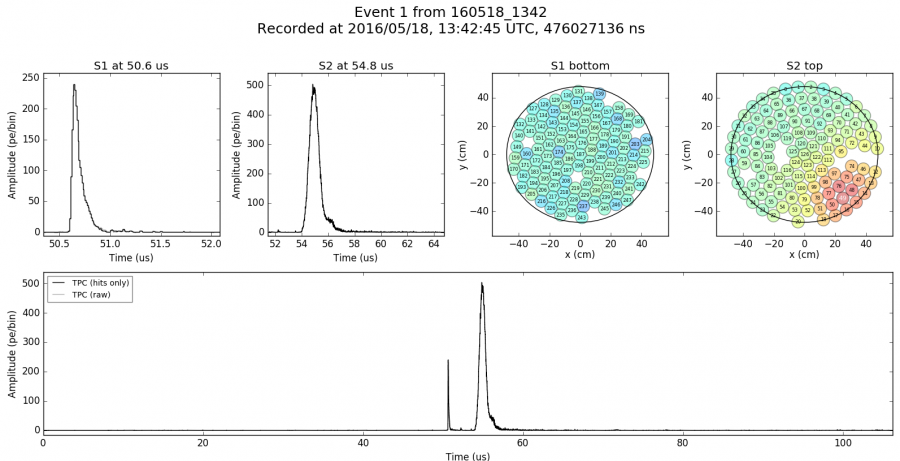
\includegraphics[width=0.99\textwidth]{tpc_waveform}
	\caption{The waveform of the first event seen by XENON1T.}
	\label{fig:tpc_waveform}
\end{figure}


\subsubsection{Detection of Scintillation Photons: S1}

The excited xenon dimers, excimers, decay very quickly (on the order of 10 ns) and produce 178 nm photons regardless of the interaction type.  These photons can be detected by the use of photomultiplier tubes (PMTs) that are designed to have peak efficiency for UV light.  In TPCs, the PMT arrays are placed at the top and bottom of the detector, as shown in \figref{fig:tpc_principle}, but cannot be placed around the sides of the TPC as the high voltage of the PMTs will prevent the electric field used to drift the electrons from being uniform in the vertical direction.  Because of this, light will typically reflect off of multiple surfaces before reaching the face of the PMT.  Since detectable light is lost during reflections, the position of the event will be important in understanding how much of the initial light is likely to be detected (with events closer to the PMTs and towards the center having a high detection efficiency than events near the edge of the TPC).  There is also an efficiency loss in the PMTs themselves since only roughly a third of photons that reach the photocathode of the PMT produce a signal --- this efficiency is referred to as the \textit{quantum efficiency} (QE).  These losses lead to roughly 90\% of light from an interaction not being detected!\footnote{Because of this large loss of scintillation light, a great deal of effort has gone into choosing and preparing material for the TPC to maximize the reflectivity \cite{silva2009reflectance, haefner2017reflectance, neves2017measurement}.}  

The main function of a PMT is to convert light signals into electrical signals, which can subsequently be digitized.  A schematic of a photomultiplier tube is shown in \figref{fig:tpc_pmt}.  When light shines upon the PMT window, there is a probability defined by the quantum efficiency that an electron is emitted by the photoelectric effect --- this electron is called a photoelectron.  This photoelectron is then guided and accelerated by an electric field to a stage of dynodes by which the initial electron produces secondary electrons at each stage in the chain.  The electrons reaching the end of the stage will be proportional to the initial number of photoelectrons and result in a current that can be digitized.  

 \begin{figure}[t]
	\centering
	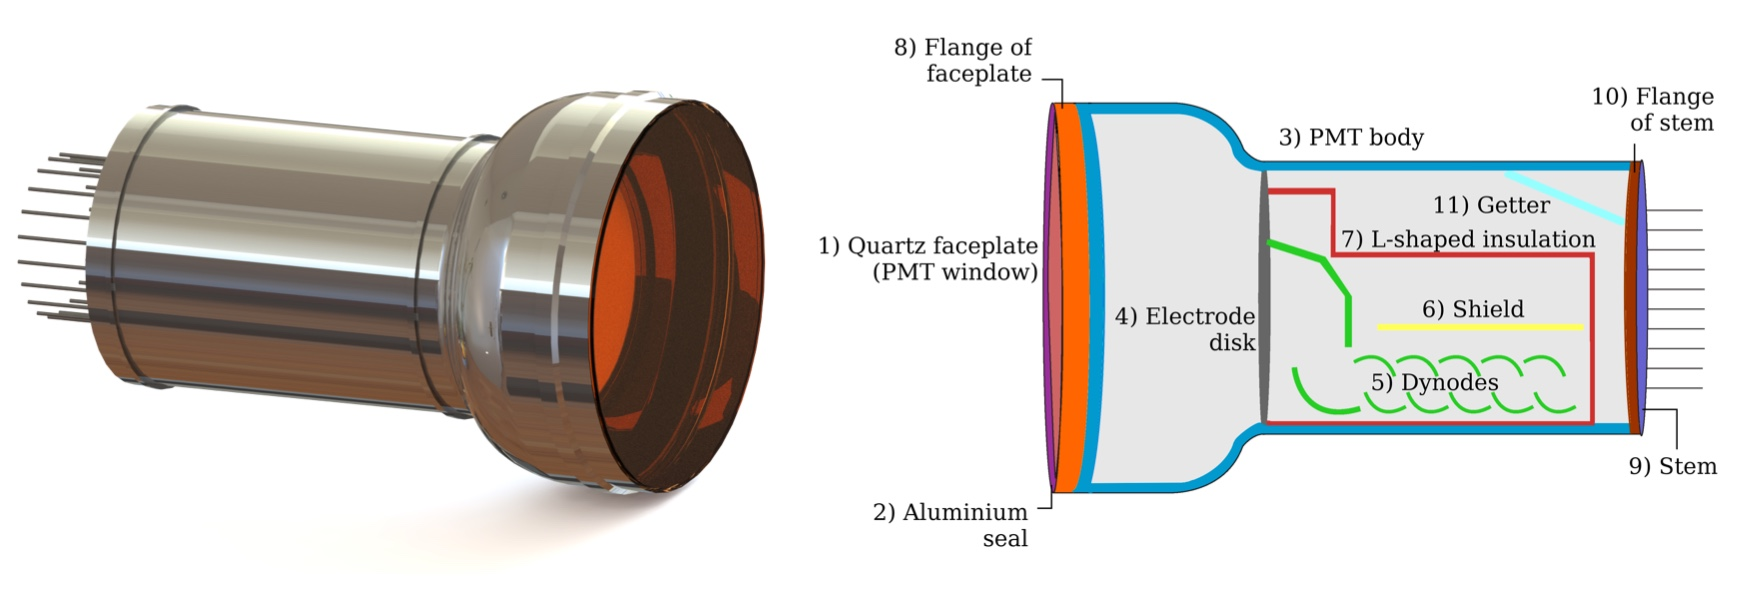
\includegraphics[width=0.99\textwidth]{tpc_pmt}
	\caption{The Hamamatsu R11410 PMT and a schematic illustration of its various components.  Image Credit: \citeref{aprile2015lowering}.}
	\label{fig:tpc_pmt}
\end{figure}

Since both the dexcitation of the excimers and the photomultiplication are both very fast processes (on the order of 10 ns), the S1 signal is considered to be a prompt signal.  This is very different from the S2 signal which will have a long delay (on the order of tens to hundreds of microseconds) depending on the depth of the interaction in the liquid xenon and the strength of the applied drift field.


\subsubsection{Detection of Ionization Electrons: S2}
\label{sec:tpc_s2_sig}

The S2 signal is a result of the electrons that do not recombine with an ion that was also created in the interaction.  These electrons are drifted using an approximately uniform vertical electric field to the liquid-gas interface and then, using a second electric field typically much stronger than the drift field (thousands of $\sfrac{\textrm{V}}{\textrm{cm}}$ compared to hundreds), are extracted from the liquid and accelerated through the gas, as shown in \figref{fig:tpc_principle}.  The accelerated electrons will create xenon excimers while being accelerated through the gas which will result in our secondary light signal that can be detected by PMTs.

The constant electron drift through the medium is actually an average over a series of many accelerations and decelerations.  The electrons are accelerated by the electric field and quickly lose energy in the liquid xenon through elastic scatters \cite{atrazhev2005electron}.  While this complicated series of interactions on a macro scale is quite simple, there is a complicating factor: electrons drifting through the liquid can be absorbed by electronegative impurities in the xenon, the most common of which is oxygen.  This process can also be examined from a larger scale and we can actually describe it with a single parameter: the so-called \textit{electron lifetime}.  The probability that an electron is not absorbed while drifting in the xenon is described in \eqnref{eqn:tpc_electron_lifetime}.

\begin{equation}
        \label{eqn:tpc_electron_lifetime}
        P(z) = \frac{1}{\tau_{e^-}} e^{-\frac{z}{v_d \tau_{e^-}}}
\end{equation}

In \eqnref{eqn:tpc_electron_lifetime}, z is the vertical distance between the electron and liquid-gas interface, $v_d$ is the drift velocity, and $\tau_{e^-}$ is the electron lifetime.  The xenon in a TPC must be constantly cleaned of these electronegative impurities to maintain a reasonable electron lifetime which proves to be technically challenging.  However, measuring the electron lifetime is relatively straight-forward.  The basic idea is that you look at an electronic recoil of known energy (the electronic recoil resulting from the decay of \ce{^{83m}Kr}, for example) and look at the S2 signal as a function of depth.   Since the light produced in the gaseous xenon is proportional to the number of electrons, one should see a decrease in the size of the S2 as a function of depth according to \eqnref{eqn:tpc_electron_lifetime}.  An example of this type of electron lifetime measurement is shown in \figref{fig:tpc_electron_lifetime}.  As detectors grow in size it is critical that they are still able to clean the xenon of the increased level of impurities still since a low electron lifetime results in a large reduction in signal and smearing in S2 (which reduces discrimination power).

 \begin{figure}[t]
	\centering
	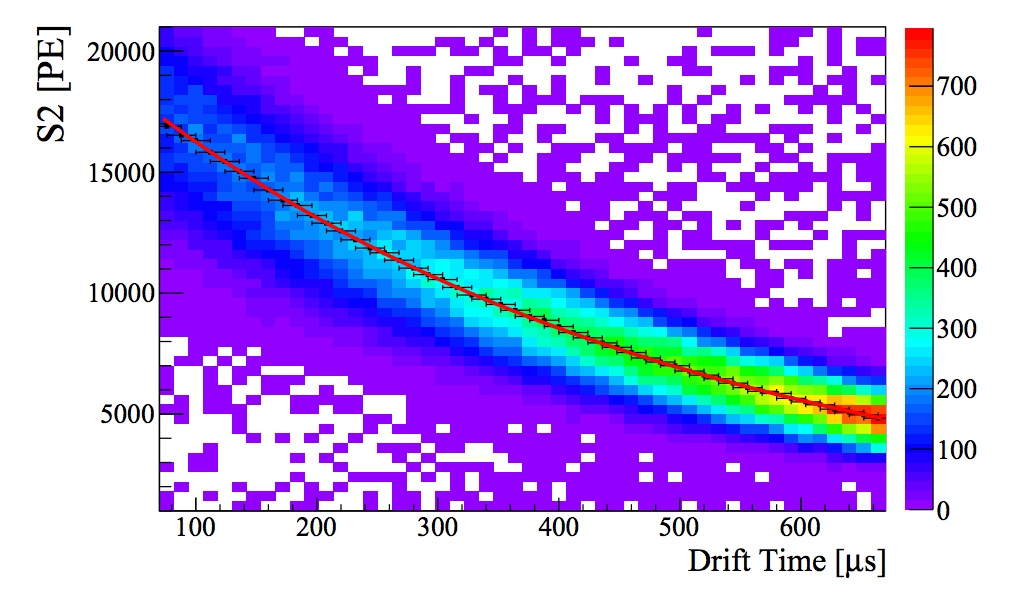
\includegraphics[width=0.99\textwidth]{tpc_electron_lifetime}
	\caption{An example of an electron lifetime analysis from XENON1T.  In this analysis, the 41 keV \ce{^{83m}Kr} electronic recoil is used and the decay's S2 signal size is plotted versus drift time (a proxy for depth).  Image Credit: \citeref{aprile2017xenon1t}.}
	\label{fig:tpc_electron_lifetime}
\end{figure}

Finally, the number of excitations produced in the gaseous xenon will be proportional to the number of electrons accelerated through.  The resulting number of photons for a single electron approximately follows a Gaussian distribution.  The mean of this Gaussian is referred to as the \textit{gas gain}.  Therefore, the number of electrons from the interaction can be inferred by looking at the number of photons detected by the photomultiplier tubes.  This quantity can also be measured in a relatively simple manner by looking at single electrons that drift to the liquid-gas interface (these single electrons often come from the photoionization of the stainless steel grids used to produce the drift field in the TPC).  This method is described in more detail in \citeref{aprile2014observation} and an example of this analysis is shown in \figref{fig:tpc_gas_gain}.

 \begin{figure}[t]
	\centering
	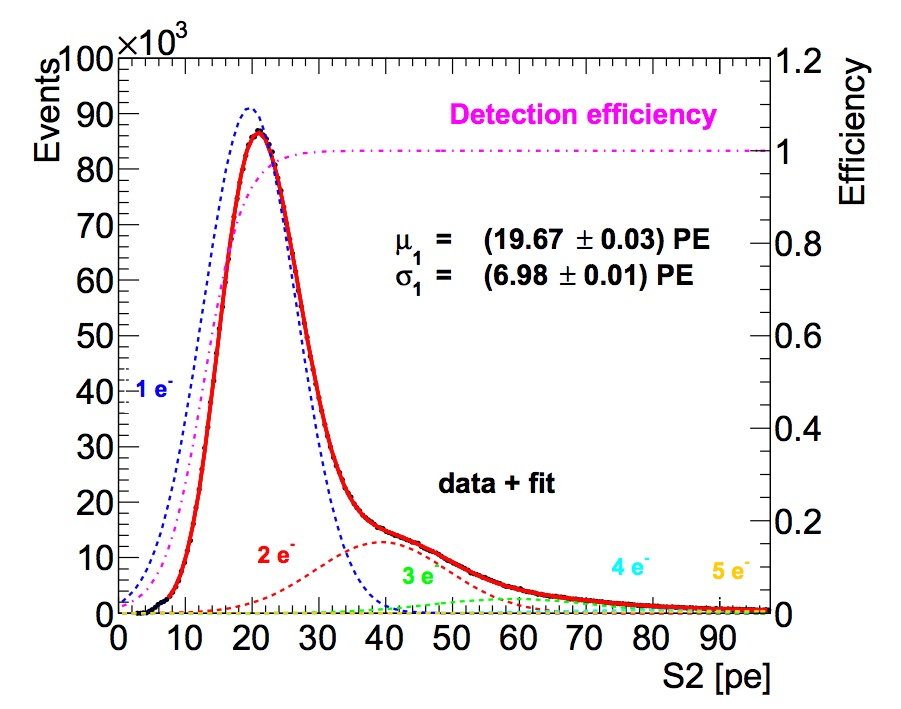
\includegraphics[width=0.8\textwidth]{tpc_gas_gain}
	\caption{An example of a gas gain analysis from XENON100.  This fit was performed using electrons from photoionization of metal inside of the detector.  Image Credit: \citeref{aprile2014observation}.}
	\label{fig:tpc_gas_gain}
\end{figure}



%This is the third chapter of the dissertation

%The following command starts your chapter. If you want different titles used in your ToC and at the top of the page throughout the chapter, you can specify those values here. Since Columbia doesn't want extra information in the headers and footers, the "Top of Page Title" value won't actually appear.

\pagestyle{cu}
\graphicspath{{./Chapter3/images/}}

\chapter[The First Dark Matter Search with XENON1T][The First Dark Matter Search with XENON1T]{The First Dark Matter Search with XENON1T}

XENON1T is the third generation detector of the XENON Dark Matter Collaboration.  With a fiducial mass of over 1,000 kg, it is expected to be the most sensitive detector in the world to WIMPs.  This chapter will focus on the XENON1T Dark Matter Experiment and the results from its first WIMP search.  The first section will focus on the design of the detector and its subsystems while the second section will focus on background considerations and estimation for the detector.  The following section will focus on the general calibration of the detector followed by a section on the calibration of the detector to nuclear recoils.  Finally, we will discuss the results of the first dark matter search and its implications.


\section{The XENON1T Detector}
\label{sec:xe1t_detector}

In this section we will focus on the XENON1T detector and its individual subsystems that are needed for it to operate according to the working principle discussed in \secref{sec:lxe_tpc}.  For more details on the design and construction of the detector, please refer to \citeref{aprile2017xenon1t}.

\subsection{ Laboratori Nazionali del Gran Sasso}

 Laboratori Nazionali del Gran Sasso (LNGS)  is an Italian national laboratory located underneath the Gran Sasso mountain range in central Italy.  In order to shield from cosmogenic backgrounds, dark matter detectors, and detectors for low background experiments in general, are placed deep underground.  Even deep underground, very high energy muons are still not completely shielded and are a dangerous background source for dark matter searches because they can produce fast neutrons in the rock that could recoil in the detector.  The flux of these neutrons at different laboratorias has been measured in \citeref{mei2006muon} and a plot of the fluxes is shown in \figref{fig:neutron_flux}.
 
 To shield against these cosmogenic neutrons, the TPC is inside the center of a cylinder filled with water that is roughly ten meters in diameter and ten meters tall.  This will be the focus of \secref{sec:muon_veto}. 
 
\begin{figure}[t]
	\centering
	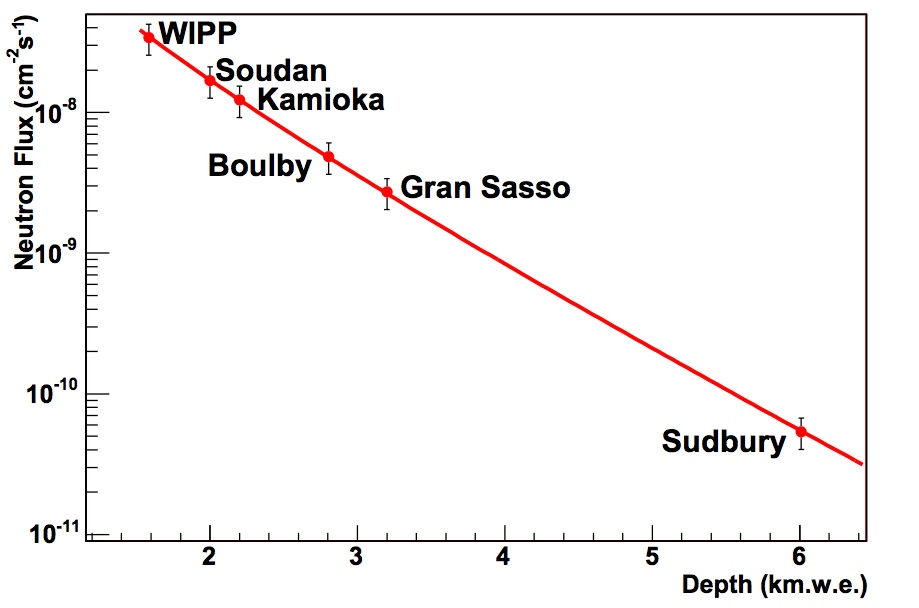
\includegraphics[width=0.8\textwidth]{neutron_flux}
	\caption{The neutron flux due to cosmogenic muons versus kilometers water equivalent depth for various underground laboratories.    Image Credit: \citeref{mei2006muon}.}
	\label{fig:neutron_flux}
\end{figure}
 
 
 \subsection{Muon Veto}
 \label{sec:muon_veto}
 
 As mentioned in the previous section, to shield against the potential cosmogenic neutron background, the TPC is placed inside of a very large water tank (~10 meter diameter and ~10 meter height).  This muon veto is outfitted with 84 8'' diameter Hamamatsu R5912ASSY high quantum efficiency PMTs to detect the light from interactions inside of the water tank and the DF2000MA reflective foil to maximize the potential measured signal \cite{aprile2014conceptual}.  A diagram showing the water tank and its PMT is shown in \figref{fig:cartoon_water_tank} and a photo of the interior of the water tank during filling is shown in \figref{fig:photo_water_tank}.  A detailed Geant4 simulation \cite{agostinelli2003geant4} of the muon events originating in the rock surrounding the laboratory shows that the efficiency of the veto is $99.78 \pm 0.05 \%$ for neutrons accompanied by the muon and $71.4 \pm 0.5 \%$ for neutrons without the initial muon.  Neutrons are accompanied by muons roughly $\sfrac{1}{3}$ of the time \cite{aprile2014conceptual}.  
 
 
 \begin{figure}[t]
	\centering
	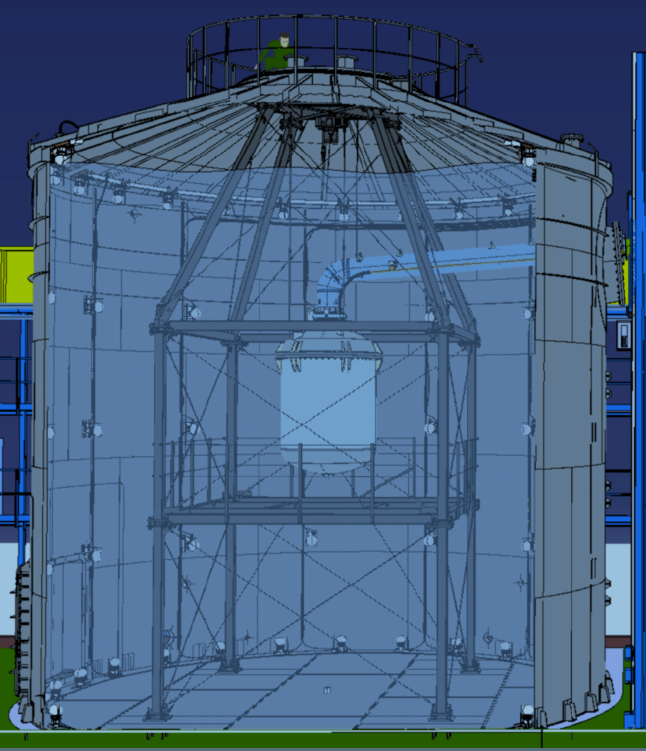
\includegraphics[width=0.6\textwidth]{cartoon_full_water_tank_muon_veto}
	\caption{A cartoon of the muon veto with the TPC centered inside the water tank.}
	\label{fig:cartoon_water_tank}
\end{figure}
 
 In addition to screening cosmogenic neutrons, the muon veto also acts as a shield to external gamma ray and neutron sources.  The neutrons mainly come from the spontaneous fission of \ce{^{238}Ur} and the \ce{^{232}Th} $(\alpha, \, n)$ reactions, both of which are found in small quantities in the surrounding rock and concrete.  Detailed Geant4 simulations \cite{agostinelli2003geant4} show that the external gamma ray background is reduced by approximately 7 orders of magnitude across 4 meters of water and the external neutron background is reduced by approximately 6 orders of magnitude per meter of water.  
 
 Given the expected fluxes for cosmogenic neutrons and radiogenic neutrons from the rock and concrete, $8.1 \cdot 10^{-10}$ above 1 MeV \cite{mei2006muon} and $8.7 \cdot 10^{-7}$ $\frac{n}{\textrm{cm}^2 \textrm{s}}$ above 1 keV, respectively, combined with the expected attenuation and cut efficiency result in a negligible external neutron background $< 0.01 \frac{\textrm{events}}{\textrm{y}}$ \cite{aprile2016physics}.
 
 
 \begin{figure}[t]
	\centering
	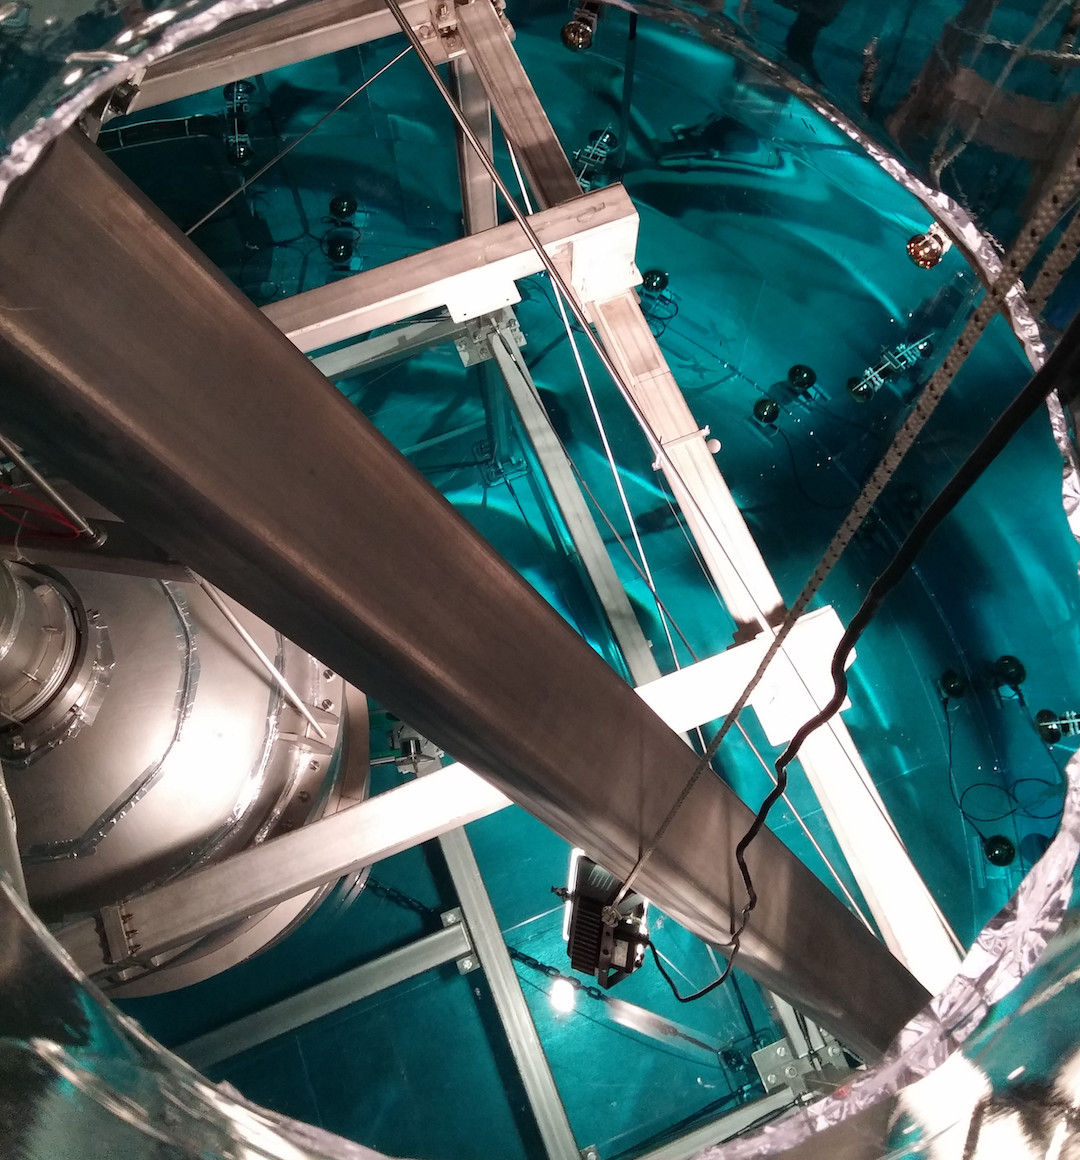
\includegraphics[width=0.6\textwidth]{water_tank_filling}
	\caption{A photo of the inside of the muon veto water tank.  The 8'' PMTs can be seen along the edges of the tank and the TPC can be seen in the center of the tank (left side of the photo).}
	\label{fig:photo_water_tank}
\end{figure}



 \subsection{Cryostat}
 \label{sec:cryostat}


In between the TPC itself and the water of the water tank is the cryostat.  The cryostat is a double-walled vacuum insulated vessel designed to contain the detector assembly and 3.5 tons of liquid xenon.  The cryostat itself is made of 5 mm thick, low radioactivity stainless steel.  The inner part of the cryostat, since it needs to house such a large amount of liquid xenon at roughly $-96^{\circ}$C, is covered in a blanket of aluminized mylar foil to minimize radiative heat transfer (shown in \figref{fig:xe1t_inner_cryostat}).  The outer cryostat is large enough to hold and support  XENON1T's inner vessel and TPC but also the inner vessel and TPC of XENONnT, a planned upgrade of XENON1T.  A diagram of the cryostat and the TPC is shown in \figref{fig:xe1t_cryostat_tpc}.

\begin{figure}[t]
	\centering
	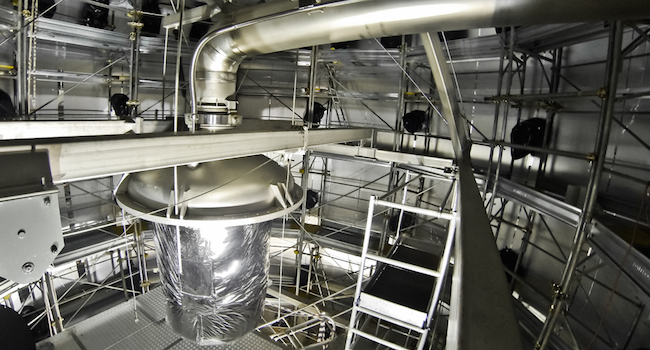
\includegraphics[width=0.99\textwidth]{xe1t_inner_cryostat}
	\caption{A photo from inside the watertank with the inner cryostat installed.  Note the mylar foil around the vessel for insulation against radiative heat transfer.}
	\label{fig:xe1t_inner_cryostat}
\end{figure}

\begin{figure}[p]
	\centering
	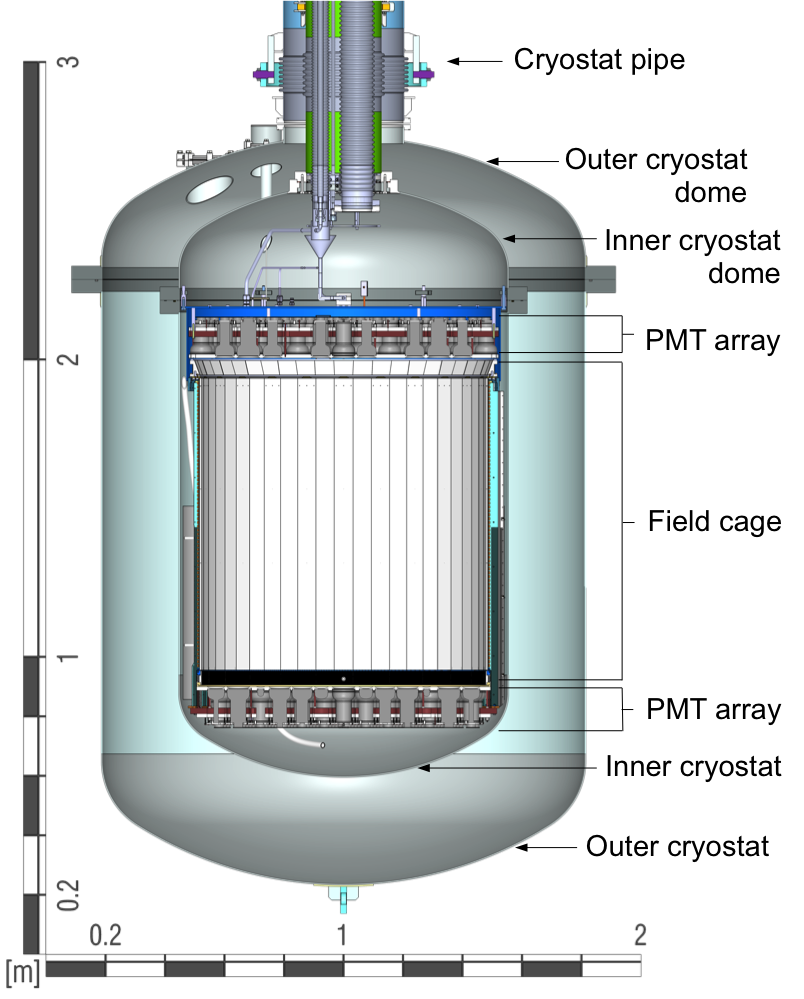
\includegraphics[width=0.99\textwidth]{xe1t_cryostat_tpc}
	\caption{A diagram of the cryostat, the TPC, and the subsystems of each.  Image Credit: \citeref{aprile2017material}.}
	\label{fig:xe1t_cryostat_tpc}
\end{figure}

The cryostat is connected to external systems such as the purification and cryogenic systems via a double-walled vacuum insulated pipe.  This pipe not only carries liquid xenon and gaseous xenon to and from the different systems but also houses the various cables that need to go into the detector (mainly signal and high voltage cables).  These cables are stored inside of a smaller pipe so that radon emanations lead away from the TPC.  One of the gaseous xenon lines is used to pressurize the xenon diving bell, which is used to set the liquid level in the detector.

The weight of the cryostat and TPC are supported by three stainless steel rods.  These rods are connected to several motion feedthroughs such that the level of the xenon in the TPC is approximately 100 $\mu$m.  These systems are also designed for XENON1T and XENONnT.

A schematic of the cryostat, TPC, and many of the subsystems that will be discussed is shown in \figref{fig:diagram_cryo_pur_sys}.


\begin{figure}[t]
	\centering
	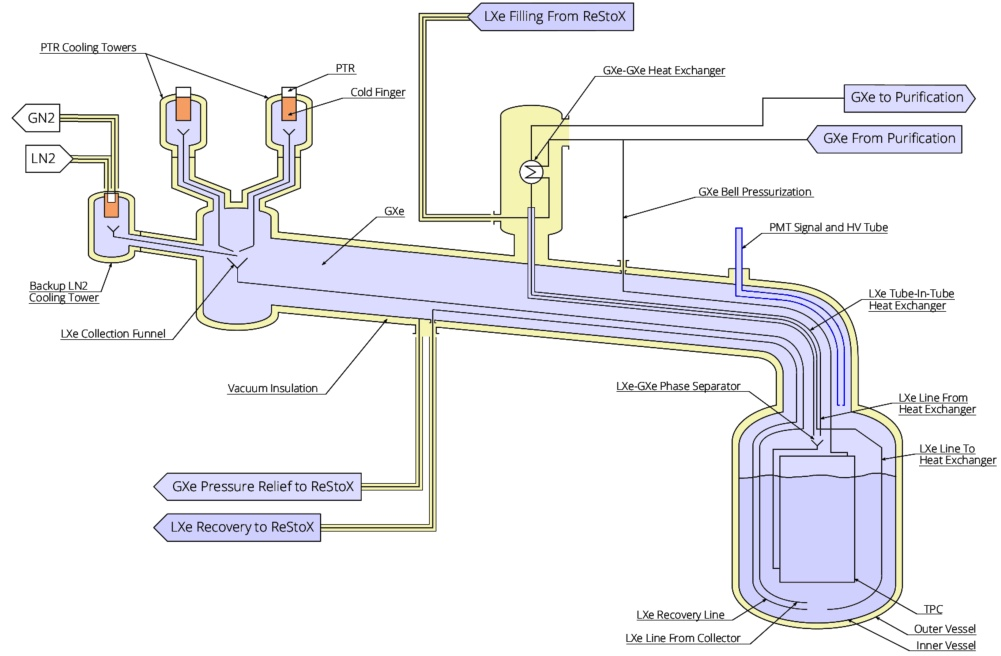
\includegraphics[width=0.99\textwidth]{diagram_cryo_pur_sys}
	\caption{A diagram of the cryostat, the cryogenics system, and the purification systems.  Image Credit: \citeref{aprile2017material}.}
	\label{fig:diagram_cryo_pur_sys}
\end{figure}


 \subsection{Cryogenics System}
 \label{sec:cryogenics_system}
 
 To keep the 3.5 tons of liquid xenon cool, two pulse tube refrigerators (Iwatani PC-150 PTRs) are used.  Each of the PTRs provides a cooling power of approximately 250 W while the estimated total heat load of the system (including the removal of electronegative impurities which will be discussed in \secref{sec:xe1t_pur_electronegative}) is less than 150 W.  Therefore, this system is doubly-redundant and designed such that a PTR can be removed and replaced during operation of the detector.  These PTRs are connected to copper cold fingers on which the gaseous xenon condensates and flows back into the detector.  The xenon pressure inside of the cryostat is controlled via resistive heaters thermally connected to the copper cold fingers.  These resistive heaters are  controlled by a proportional-integral-derivative (PID) controller that adjusts the power of the heaters to maintain a desired cold-finger temperature \cite{aprile2017xenon1t}.
 
 The photomultiplier tubes (which will be discussed in \secref{sec:photomultiplier_tubes}) are susceptible to damage if the pressure in the detector becomes too high.  For this reason, it is crucial to be able to keep the pressure stable even in the event of an emergency.  XENON1T was designed such that if there is a sudden increase in pressure, a cold finger that is cooled using liquid nitrogen is used in place of the PTRs.  To maintain normal operating conditions in the detector only ~100 liters per day are required (the tank containing liquid nitrogen can store up to 10 $\textrm{m}^3$) \cite{aprile2017xenon1t}.
 
 The three redundant cooling systems can be seen on the left side of \figref{fig:diagram_cryo_pur_sys}.  The gas in the pipe condenses on the cold fingers and then is fed back into the cryostat.

 
 \subsection{Purification Systems}
 \label{sec:xe1t_pur}
 
 There are two main purification systems in XENON1T: one for electronegative impurities and a second for the removal of \ce{^{85}Kr}.  
 
 \subsubsection{Electronegative Impurities}
 \label{sec:xe1t_pur_electronegative}
 
 As mentioned in \secref{sec:tpc_s2_sig}, electronegative impurities, mainly oxygen, enter the liquid xenon through the various materials used when constructing the detector.  These electronegative impurities can capture free electrons that are drifted to produce the secondary signal, the S2.  This causes a complete loss of signal in the case of high concentrations but will still causes large smearing effects at low levels of concentration (ppb levels of \ce{O_2} relative to xenon), reducing the discrimination power of liquid xenon for electronic and nuclear recoils.
 
Materials are cleaned before being installed in the detector however these electronegative impurities are constantly outgassing into the detector and therefore the xenon must be constantly cleaned.  To achieve high purity, a doubly redundant purification system that is connected to the cryostat is used (center of \figref{fig:diagram_cryo_pur_sys}).  This system includes two loops with a gas driving pump (CHART QDrive) and a high-termperature arare-gas purifier (SAES PS4-MT50-R getter) \cite{aprile2017xenon1t}.  The SAES getter is able to reduce the \ce{O_2}, \ce{H_2O}, \ce{CO}, \ce{CO_2}, \ce{H_2}, \ce{N_2}, and \ce{CH_4} concentrations to low ppb or below by having the impurities form irreveersible chemical bonds with the material inside of the getter.  One drawback of the getter is that it must be operated at high temperatures ($\sim 50^{\circ} \, \textrm{C}$).  However, this effect can be reduced by using heat exchangers between both the hot and cold liquid and gaseous xenon.  The gaseous heat exchanger can be seen in the center of  \figref{fig:diagram_cryo_pur_sys} and the liquid heat exchanger (tube-in-tube) can be seen on the right side of \figref{fig:diagram_cryo_pur_sys}.  These heat exchangers are approximately 96\% efficiency and significantly reduce the heat input of the getters to 0.39 $\sfrac{\textrm{W}}{\textrm{SLPM}}$ \cite{aprile2017xenon1t}.

% getter specs: http://www.saespuregas.com/Library/specifications-brochures/s110-233_a_521.pdf
 
 
 \subsubsection{\ce{^{85}Kr}}
  \label{sec:xe1t_pur_kr85}
 
 A cryogenic distillation column is used to reduce the natural krypton to xenon level to below 200 ppq (part per quadrillion).  The cryogenic distillation column leverages the different vapor pressures of the two elements around the xenon boiling point: the vapor pressure of krypton is roughly 10.8 times higher than the vapor pressure of xenon at 175 K and 2 bars.  For a dual-phase system in equilibrium, this implies that the gaseous phase will be enriched with krypton relative to the liquid by this factor of 10.8 --- this simple dual-phase system is referred to as a single distillation stage.  To improve this separation efficiency, one can put several of these distillation stages in series with each other.  This multi-stage distillation column can practically be achieved via a package material that replicates these additional stages when placed inside of a single stage.  The height of the material ultimately translates into the number of stages added \cite{fieguth2016distillation}.
 
 The concentration can be measured with an RGMS (residual gas mass spectrometer) or an RGA (residual gas analyzer).  A distillation column with 2.8 meters of the Sulzer EX package material was deployed for XENON1T and achieved natural krypton to xenon levels of $< 48$ ppq \cite{aprile2017removing}.  
 
 A similar distillation column was also built to test the possibility of radon removal.  Using 1 meter of package material, a radon reduction factor of $>$ 27 was achieved \cite{aprile2017online}.
 
 
  \subsection{Recovery and Storage}
 
 For small detectors, it sufficed to fill detectors via cooling the xenon stored in bottles and to empty the detector by evaporating the liquid xenon.  While simple, this method is inefficient and would require approximately 250 W of heating power over 2 months to fill the XENON1T detector \cite{aprile2017xenon1t}.  While an emergency situation is unlikely in XENON1T due to its many redundancies, this simple method would also make recovery of all of the xenon very difficult.
 
 Instead of storing unused xenon in bottles kept at room temperature, a new approach to recovery and storage of xenon was applied: a single 5 cubic meter vacuum-insulated stainless steel sphere rated for pressures up to 73 bar was built for this purpose, appropriately name RESToX (recovery and storage of xenon).  Similar to the detector's cryostat, several layers of aluminized mylar blanket the inner wall of this system such that the heat load on this system is only roughly 50 W.  RESToX is cooled using 16 liquid nitrogen lines that are welded to the outside of the inner wall.  To assure that the xenon inside of RESToX is kept at a precise temperature and pressure (to avoid freezing), a heating system has also been installed in the center of the vessel.
 
 RESToX is directly connected to the cryostat for filling and recuperation of the xenon gas as well as both purification systems such that the xenon stored can be kept clean and ready for use.  Xenon can be transferred into the cryostat via the pumps of the purification system (up to a maximum speed of 50 SLPM). Xenon is transferred from the cryostat to RESToX solely due to the pressure difference between the two systems.
 
 \begin{figure}[t]
	\centering
	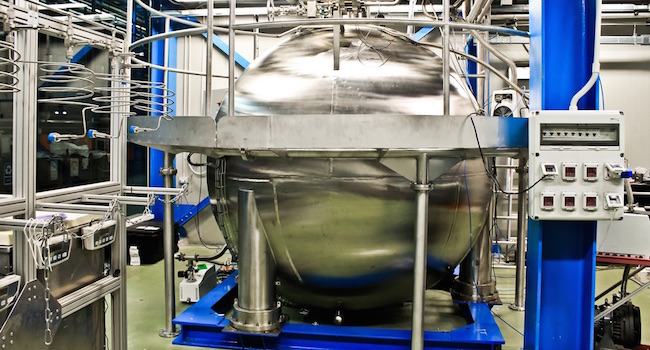
\includegraphics[width=0.99\textwidth]{xe1t_restox}
	\caption{A photograph of RESToX prior to instillation at LNGS.}
	\label{fig:xe1t_restox}
\end{figure}


  \subsection{Calibration Systems}
 \label{sec:xe1t_calibration_system}
 
While, like LUX \cite{akerib201783}, internal sources, such as \ce{^{83m}Kr}, can be injected through the purification system, a new method for introducing external sources needed to be developed due to the massive water tank surrounding the TPC.  The solution was the installation of two belts that could be used to move external sources around the bottom of the detector (the ``U-Belt'') and along the sides of the detector (the ``I-Belt'') and an additional mechanism to move the neutron generator vertically along the side of the TPC.  The main external sources used are \ce{^{228}Th} (which has several $\gamma$ lines between 511 -- 2,614 keV), \ce{^{137}Cs} (which has a single $\gamma$ line at 662 keV), and AmBe (which produces MeV energy neutrons).  The neutron generator (NSD Gradel Fusion NSD-35-DD-C-W-S) uses the deuterium-deuterium fusion process to create neutrons with energies between 2.2 and 2.7 MeV.  This generator has been specially designed to provide very low neutron rates ($\mathcal{O} \left(10 \, \sfrac{\textrm{n}}{\textrm{s}} \right)$) as well as high neutron rates ($\mathcal{O} \left(10^6 \, \sfrac{\textrm{n}}{\textrm{s}} \right)$).  These external source systems are shown in \figref{fig:xe1t_external_sources}.

Like previous generations of detectors, the PMTs are calibrated using pulsed blue light fed into the detector by fiber optic cables.  In XENON1T, four such fiber optic cables are fed into the detector at different heights and positions.


 \begin{figure}[t]
	\centering
	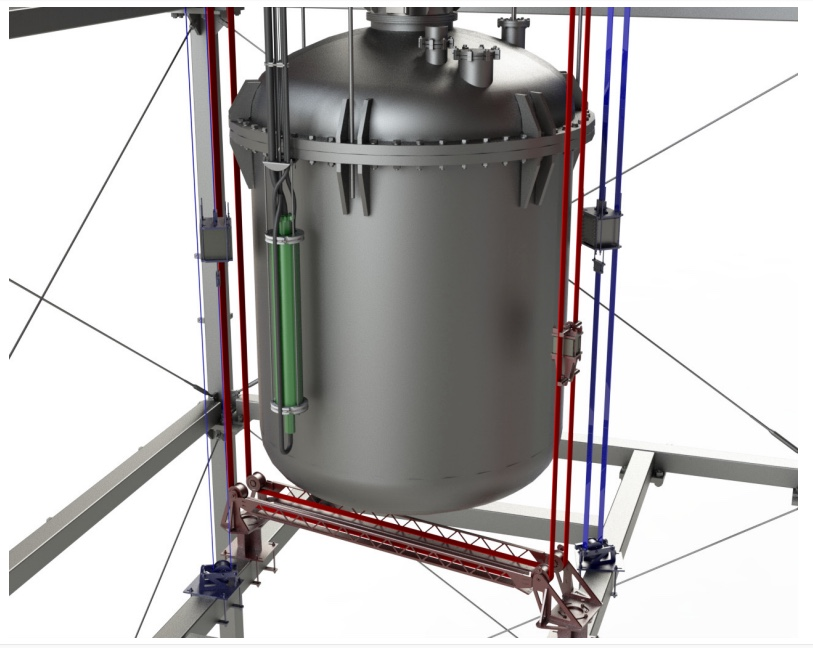
\includegraphics[width=0.7\textwidth]{xe1t_external_sources}
	\caption{A diagram showing the external calibration systems.  The ``U-Belt'', which allows for placement of external sources below the TPC, is shown in red while the ``I-Belt'', which allows for the placement of external sources at different heights along the side of the TPC, is shown in blue.  Shown in green is the neutron generator which can be raised an lowered along the side of the detector.}
	\label{fig:xe1t_external_sources}
\end{figure}
 
 
 \subsection{Photomultiplier Tubes}
 \label{sec:photomultiplier_tubes}
 
XENON1T utilizes a total of 248 high quantum efficiency  R11410-21 3 inch PMTs --- 127 of these PMTs are located in the top array and the remaining 121  are located in the bottom array.  The R11410-21 was specifically designed for XENON1T to have a high quantum efficiency, high collection efficiency, low radioactivity, and operate stably at liquid xenon temperatures.  

321 of the R11410-21 PMTs were tested for quantum efficiency, dark rate, stability, and single photoelectron response.  Of the 321 PMTs, 78 were rejected: 12 due to high or unstable dark count rate and 53 due to after-pulsing (44 of which were confirmed to have a leak).  The PMTs were found to have an average quantum efficiency of $34.5 \pm 2.8 \%$ at 178 nm and a collection efficiency of $90 - 95 \%$ \cite{barrow2017qualification}.  PMTs that were found to have a higher quantum efficiency and collection efficiency were placed in the center to maximize potential light collection as shown in \figref{fig:xe1t_pmt_qe}.  The bottom PMT array sees the majority ($\sim 90\%$) of the light for S1s due to the reflection of light at the liquid-gas interface --- therefore, the higher quantum efficiency PMTs were placed in the bottom array.

\begin{figure}[t]
	\centering
	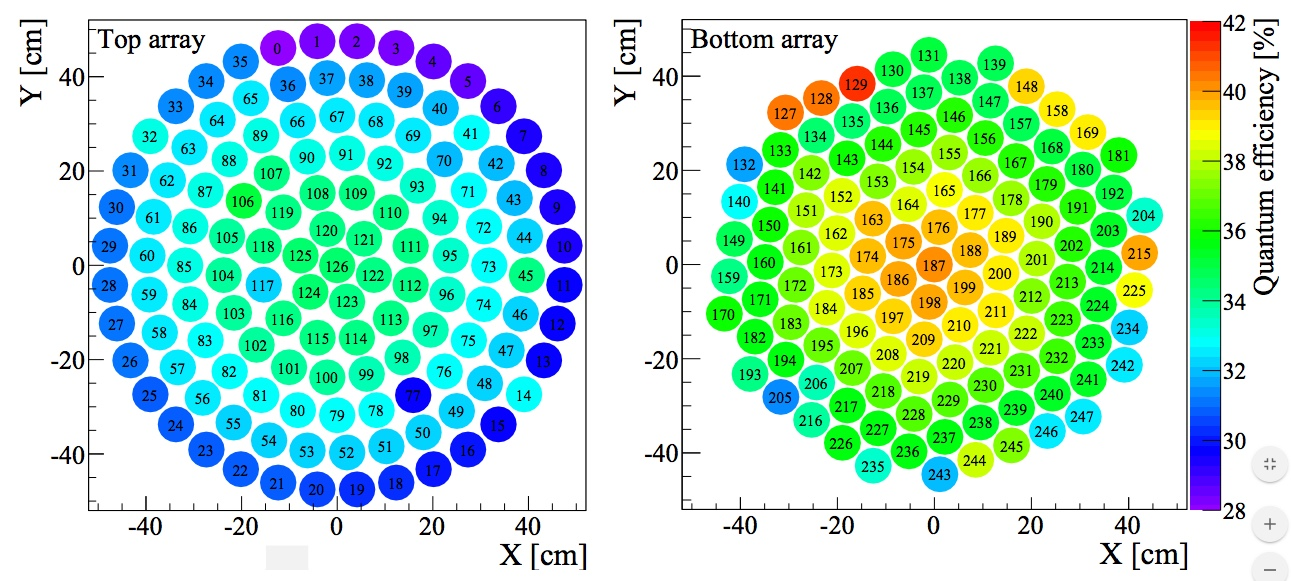
\includegraphics[width=0.99\textwidth]{xe1t_pmt_qe}
	\caption{The quantum efficiencies of the PMTs installed in the XENON1T PMT arrays.  Note that, with a few exceptions due to higher radioactivity levels, the highest quantum efficiency PMTs are placed towards the center to maximize light collection.  Also note that in general the PMTs used in the bottom array have a higher quantum efficiency than those in the top array since the much smaller S1 signal is mainly seen by the bottom array.  Image Credit: \citeref{aprile2017xenon1t}.}
	\label{fig:xe1t_pmt_qe}
\end{figure}
 
 Of the 248 PMTs installed, only 213 could be used for the first science run of XENON1T.  The reasons for omission in the final analysis varied from high levels of noise, frequent trips and flashing, and low single photoelectron acceptance at the trigger threshold.  The remaining PMTs were set such that they had a gain from $2- 5 \cdot 10^6 \, \textrm{e}^-$ and a resolution of approximately 30\%.  The gains of individual PMTs were stable over the course of data taking.
 
 % mention work on characterization of PMTs in later chapter
 
  \subsection{XENON1T TPC}
 \label{sec:xe1t_tpc}

The XENON1T has a cylindrical shape with a diameter of 96 cm and height of 97 cm at room temperature.  The TPC outer wall is made of PTFE (polytetrafluoroethylene), otherwise known as teflon.  Teflon is chosen for several reasons: it has a high reflectivity, it can be made such that it is highly radio-pure, it has low outgassing rates, it is chemically inert (so no special considerations need to be made for handling or storage), and it is an excellent insulator \cite{neves2017measurement}.  Teflon does have a high thermal coefficient of expansion resulting in a length contraction of approximately 1.4\% from room temperature to liquid xenon temperatures \cite{kirby1956thermal}.

Throughout this and second half of the previous chapter, it has been assumed that one can provide a uniform drift field in the TPC in order to extract the electrons from the interaction site to the liquid-gas interface and a uniform extraction field to extract the electrons from the liquid into the gas for amplification.  Ideally, one would use sets of parallel plates to create these uniform fields however this has the obvious drawback of not allowing for the detection of light.  Instead, the plates are replaced with ultrafine grids that can approximate a uniform field while keeping a high transparency ($\gtrapprox 90 \%$ from optical simulations).  The width of the wires used in the grids is $\mathcal{O}(0.2 \, \textrm{mm})$ and the size of the cells in the grid is $\mathcal{O}(5 \, \textrm{mm})$.  To create the two fields mentioned, the drift and extraction fields, we need three meshes: the cathode mesh ($\mathcal{O}(10-100 \, \textrm{kV})$), the gate mesh (ground), and the anode mesh ($\mathcal{O}(5 \, \textrm{kV})$).  To protect the PMTs from the high electric field, screening meshes kept at similar voltages to the PMTs ($\sim -1.5$ kV) are also installed.  To reduce edge effects and keep the field as uniform as possible out to the edge of the TPC, 74 field shaping rings made of oxygen-free high thermal conductivity copper are installed between the cathode and the anode via a chain of 5 G$\Omega$ resistors \cite{aprile2017xenon1t}.  Shown in \figref{fig:xe1t_sr0_field_sim} are the field simulations made using the final detector design and the voltages used during the first science run of XENON1T ($V_c = -12 \, \textrm{kV} \textrm{ and } V_a = 4 \, \textrm{kV}$).  

% cathode:12 kV in SR0
% anode: 4 kV
% screening: -1.55 kV (top and bottom)


\begin{figure}[t]
	\centering
	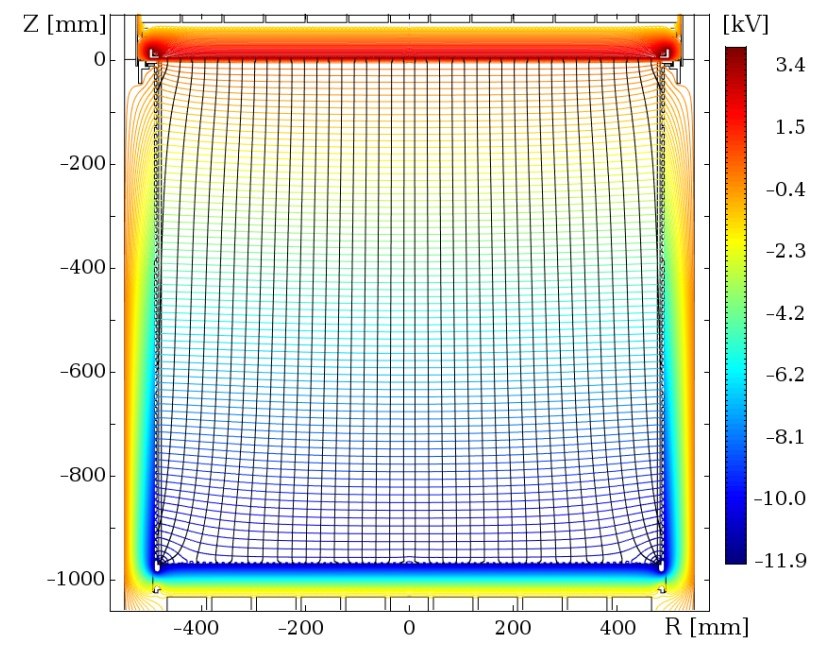
\includegraphics[width=0.99\textwidth]{xe1t_sr0_field_sim}
	\caption{The field simulations for the TPC during the first science run of XENON1T.  During this run, a cathode voltage of $-12$ kV was used and an anode voltage of $+4$ kV was used.  Image Credit: \citeref{aprile2017xenon1t}.}
	\label{fig:xe1t_sr0_field_sim}
\end{figure}


\subsection{Data Acquisition and Processing}
\label{sec:xe1t_daq_pax}

The final subsystem of XENON1T is the detector acquisition and processing system.  The signals from the 248 TPC PMTs and 84 muon veto PMTs, after being amplified by a factor of ten using a Phillips Scientific 776 Amplifier, are fed into V1724 flash ADCs.  These V1724 ADCs operate at 100 MHz (resulting in a time resolution of 10 ns), with 14 bit resolution, 40 MHz bandwidth, and a 2.25 or 0.5 V dynamic range.   Each ADC can handle eight channels simultaneously \cite{caen2017v1724}.  

The data acquisition does not have an external trigger --- instead, all pulses are digitized for each channel.  The pulses for each channel are then analyzed together to determine whether or not an event occurred and should be saved.  These events (saved as \textit{waveforms} that are just ADC counts versus time) can then be processed to extract relevant information, including, but not limited, to the size of S1 and S2 signal.  The processor, \textit{PAX} (Processor for Analyzing Xenon), was designed for XENON1T but is portable enough to be used for other dual-phase TPCs. %The efficiency of saving events using this method is found, via simulation, to be approximately 100\% after only two electrons are accelerated through the gaseous xenon given the anode voltage for the first science run.  % S1 efficiency 

Since the expected WIMP energy spectra (and most of the nuclear recoil background sources) exponentially decay with energy, it is crucially important to understand the efficiency with which events are saved and S1s and S2s are found in the events by the processor.  For the coincidence conditions, thresholds, and algorithms used in the first science run of XENON1T, it was found via simulation that S2s are identified with 100\% efficiency when produced with two or more electrons accelerated through the gaseous xenon.  This implies that even the smallest events are successfully saved.  However, given the threshold and algorithm choices of the first science run, it was found, again via simulation, that five or more photons are needed to correctly identify an S1 for an event with above an 80\% probability.  Therefore, even with the event saved, we may not be able to extract the necessary information since the processor cannot identify the S1 in the waveform.  These efficiencies will be discussed in more detail with respect to the nuclear recoil calibration of XENON1T.

\begin{figure}[t]
	\centering
	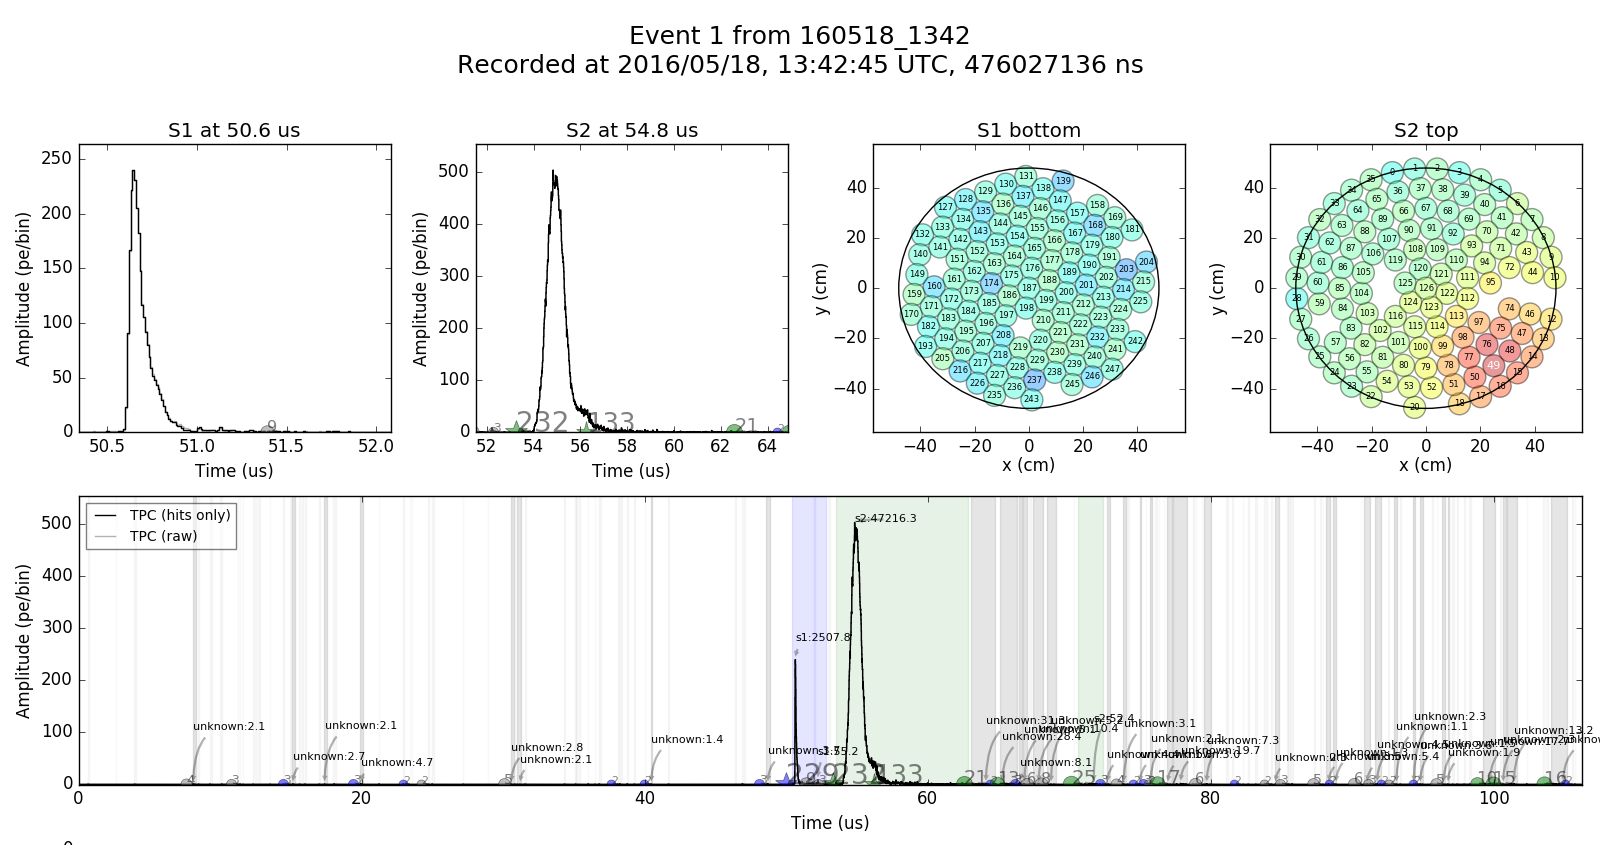
\includegraphics[width=0.99\textwidth]{xe1t_pax_output_first_waveform}
	\caption{The PAX output for the first waveform in XENON1T.  Shown in blue is the S1 and shown in green is the S2.  The grey highlighted areas represent unidentified peaks that are likely due to the high noise rate at this point in the detector operation.  Also shown are the timestamps of each signal, used to extract the depth of the interaction, and the PMT hit patterns of the top and bottom PMT arrays, which are used for position reconstruction.}
	\label{fig:xe1t_pax_output_first_waveform}
\end{figure}


\section{The Background for the XENON1T Detector}
\label{sec:xe1t_bkg}

Many of the potential sources of background were first discussed in the second chapter.  In this section we quantify the expected rate of each of these sources as a function of energy.  As mentioned previously, the higher the expected rate of background is in your region of interest, the harder it is to make a claim that excess events are due to WIMPs.  


\subsection{Background in XENON1T from Detector Materials}
\label{sec:xe1t_materials_bkg}

The first source of background that we will discuss is from the detector materials themselves.  The detector material background contributes to both the electronic and nuclear recoil background.  Even though incredible care is taken to select the most radiopure detector components for the detector, this background will prove to be non-negligible for XENON1T, as with all other dual-phase TPCs.

To quantify the background from the different detector components, materials were screened using a high-purity germanium detector and using mass spectrometry.  A detailed breakdown of the radioassay results of the various detector materials can be found in \citeref{aprile2017material}.  To estimate the background, the twelve largest background contributors and the eight most relevant backgrounds are considered \cite{aprile2016physics}.  We can simulate the background by assuming the contaminants are spread uniformly in the various detector materials and by requiring the interaction occur inside of a fiducial volume and with only a single scatter in the liquid xenon volume.  The resulting energy spectrum from the simulation for electronic recoils can be seen in \figref{fig:xe1t_er_bkg_all} and \figref{fig:xe1t_er_bkg_low} and the resulting energy spectrum from the simulation for nuclear recoils can be seen in \figref{fig:xe1t_nr_bkg}.  Each of these spectra can be integrated to determine the rate per kilogram of xenon in the fiducial volume per day.


\subsection{Electronic Recoil Background in XENON1T}
\label{sec:xe1t_er_bkg}

Even though electronic recoils can be rejected with high confidence due to their larger charge signal relative to nuclear recoils, they still pose a dangerous background for dark matter searches since the electronic recoil and nuclear recoil band overlap (as seen in \figref{fig:xe1t_disc}).  Putting aside the possibility that dark matter may interact with atomic electrons, in which case this is our most relevant background, a higher  overall rate of electronic recoils in our detectora translates to a higher probability of an electronic recoil mimicking a nuclear recoil (simply from statistical fluctuations).

The full electronic recoil background energy spectrum can be seen in \figref{fig:xe1t_er_bkg_all} and \figref{fig:xe1t_er_bkg_low}.  It is important to recall that since electronic recoils efficiently convert energy into observables, only electronic recoils under 15 keV are relevant to the WIMP search.  We will briefly discuss each component of the background in the remainder of this section with the exception of the materials background, which is discussed in \secref{sec:xe1t_materials_bkg}.

%\begin{figure}[t]
%	\centering
%	\subfloat{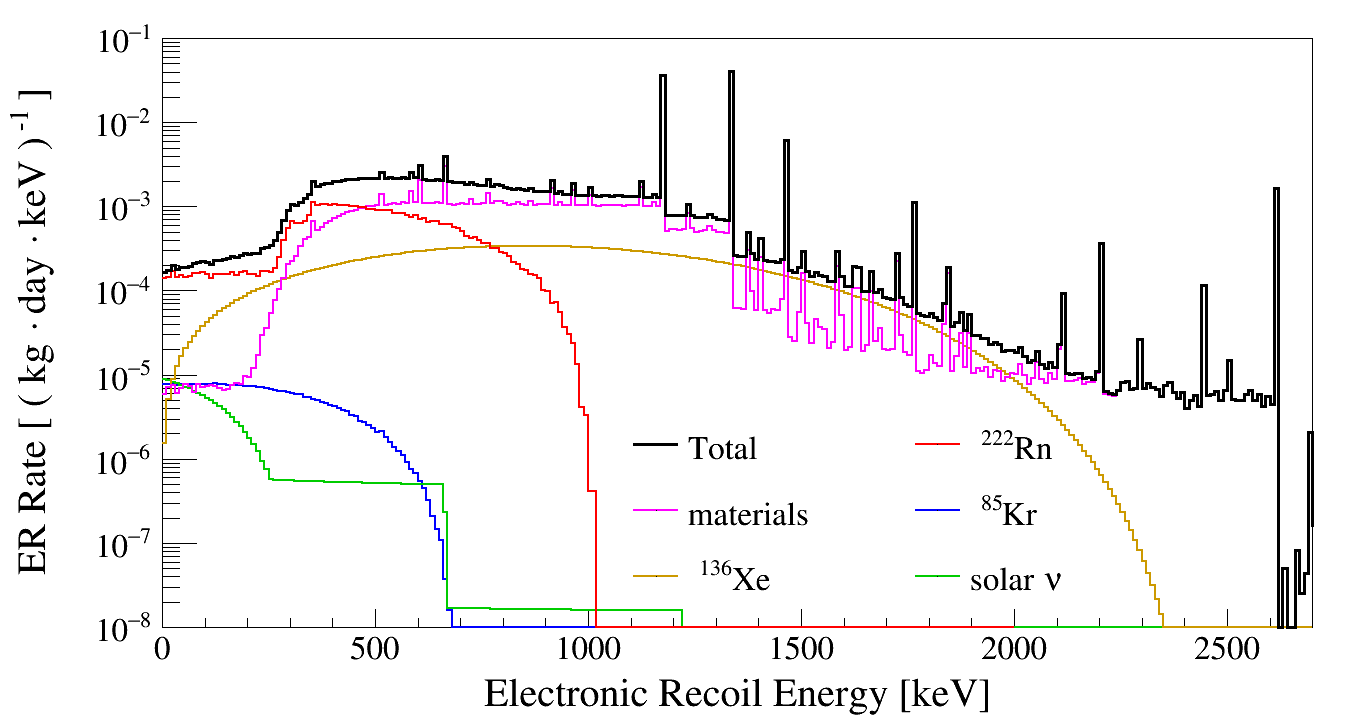
\includegraphics[width=0.5\textwidth]{xe1t_all_energy_er_bkg}} \hfill
%	\subfloat{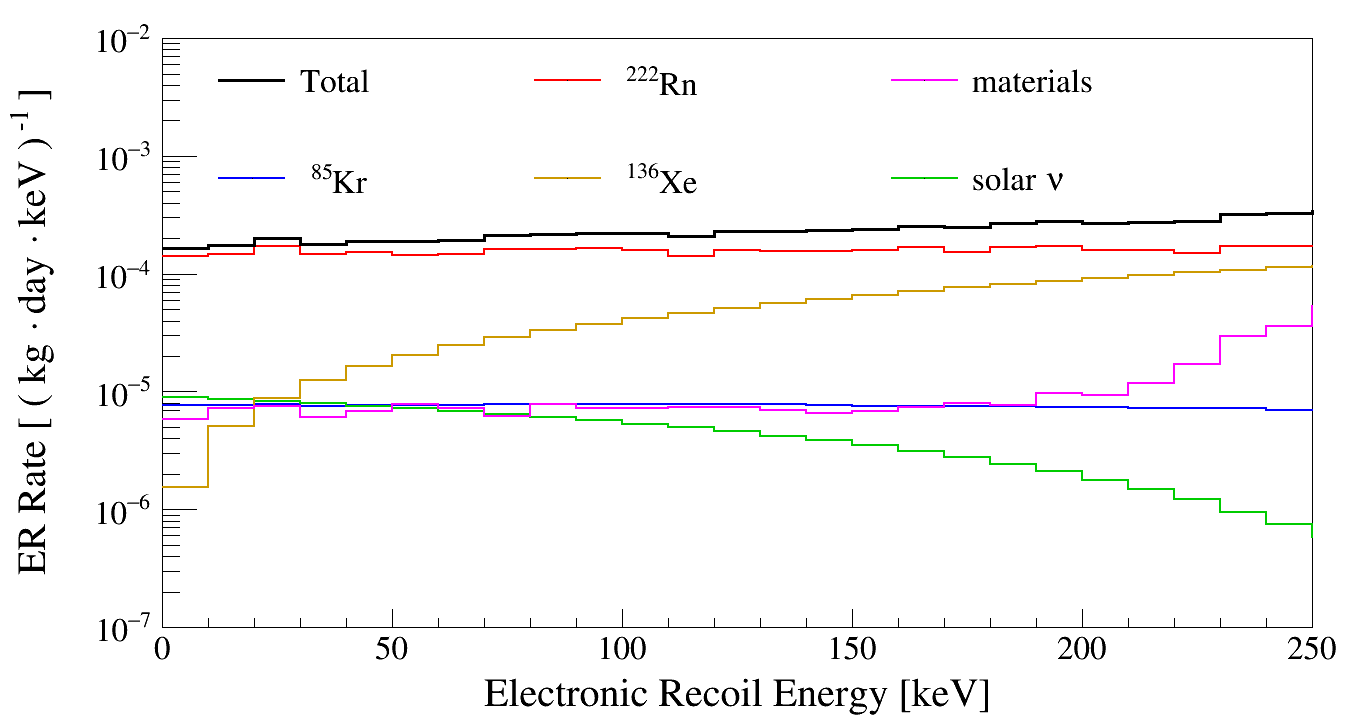
\includegraphics[width=0.5\textwidth]{xe1t_low_energy_er_bkg}}
%	\caption{.  Image Credit: \citeref{aprile2016physics}.}
%	\label{fig:xe1t_pax_output_first_waveform}
%\end{figure}


\begin{figure}[p]
	\centering
	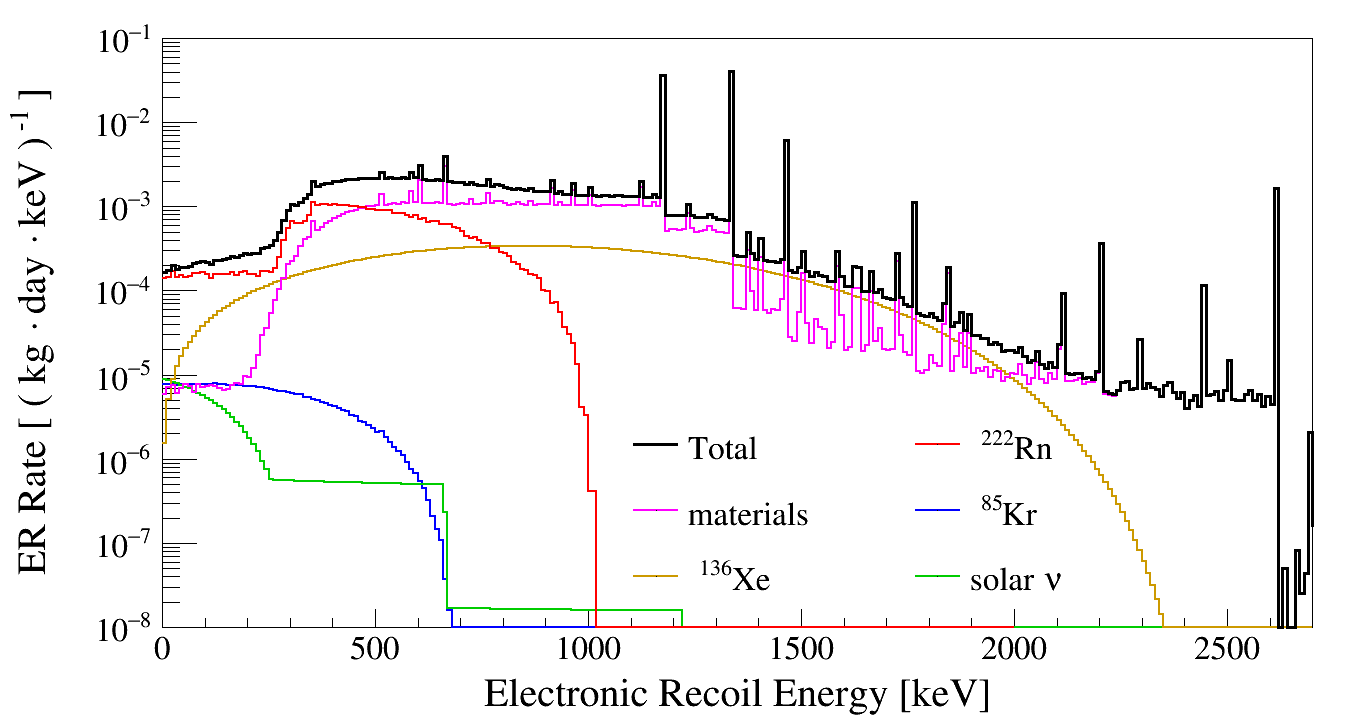
\includegraphics[width=0.95\textwidth]{xe1t_all_energy_er_bkg}
	\caption{The electronic recoil energy spectrum expected from major background sources.  While radiation from materials and the double beta decay of \ce{^{136}Xe} dominate at high energies, \ce{^{222}Rn} dominates at the lowest energies as can be seen here and in \figref{fig:xe1t_er_bkg_low}.  This low energy region is of the most concern for dark matter searches.  Image Credit: \citeref{aprile2016physics}.}
	\label{fig:xe1t_er_bkg_all}

        \vspace{\floatsep}

	\centering
	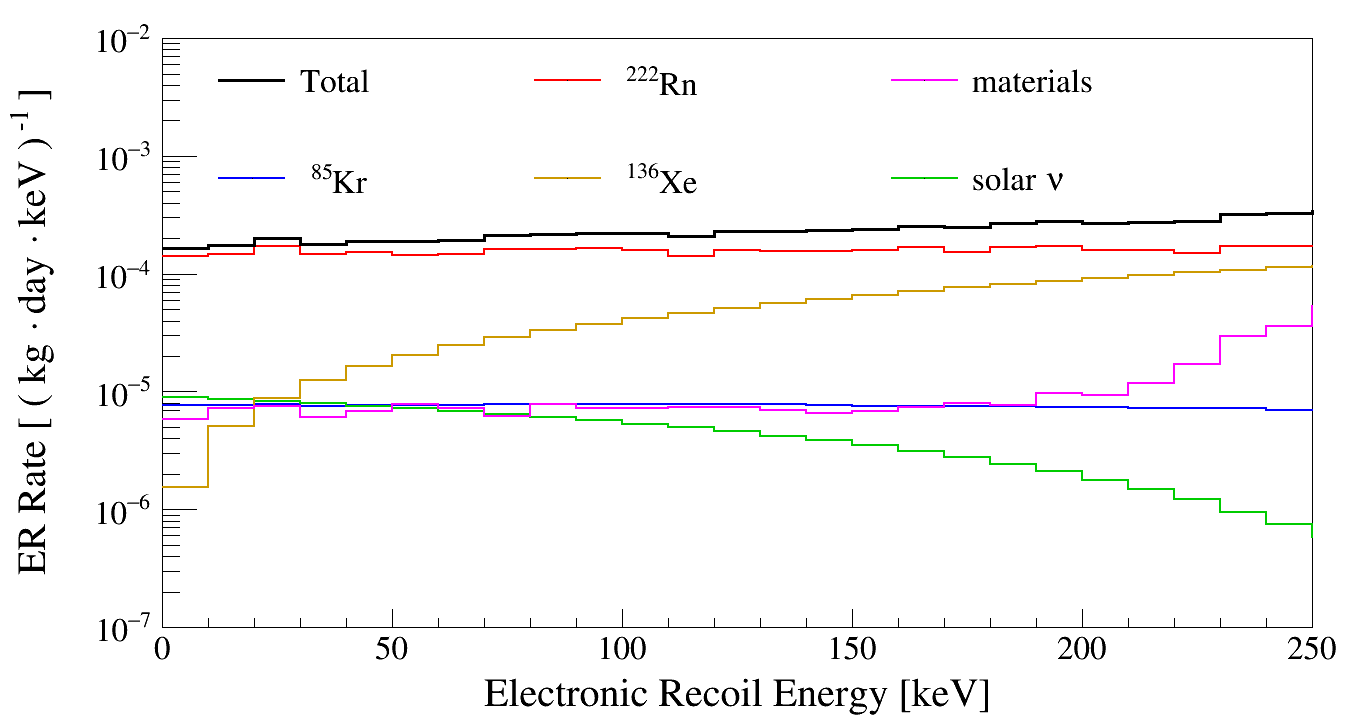
\includegraphics[width=0.95\textwidth]{xe1t_low_energy_er_bkg}
	\caption{The electronic recoil energy spectrum from background at low energies.  Note that under 15 keV, the upper threshold for electronic recoils relevant to the dark matter search, \radon{} is the dominant source of electronic recoils.  Image Credit: \citeref{aprile2016physics}.}
	\label{fig:xe1t_er_bkg_low}
\end{figure}


\subsubsection{\ce{^{222}Rn}}
\label{sec:xe1t_er_rn222}

Radon, unlike all of the other noble gasses, has no stable isotope.  Therefore, ``natural'' radon is the result of the $\alpha$ decays of \ce{^{226}Ra} into \radon{} and \ce{^{224}Ra} into \ce{^{220}Rn}.  These maternal isotopes are part of primordial \ce{^{238}U} and \ce{^{232}Th} chains, respectively, that are shown in \figref{fig:xe1t_rn_decay_chains}.  

However similar these two chains might seem, they prove to have drastically different effects for dark matter detectors.  Both \uranium{} and \thorium{}, and therefore their daughter isotopes, are found in trace quantities in almost all materials, including the ones used for the construction of XENON1T.  When either chain reaches the decay of radium into radon, the recoiling radon isotope has a chance of emanating from the surface that it is found on, for example from the inside of a stainless steel pipe into the gaseous xenon.  This is where the difference in the two chains materializes itself.  First, notice that the \uranium{} chain essentially ends at \ce{^{210}Pb} because of its long half-life.  Second, notice that with the exception of \ce{^{214}Pb} and \ce{^{212}Pb} all decays are either $\alpha$ decays or $\beta$ decays in close coincidence with an $\alpha$ decay such that events can be tagged and cut.  These two isotopes of lead both beta decay with continuous energy spectra down to zero energy, making them both potentially dangerous background.  However, the decays leading to and the decay of \ce{^{212}Pb} are relatively quick (55 seconds, 0.14 seconds, and 10.6 minutes) --- this implies that the \ce{^{212}Pb} will still be almost entirely concentrated at the edge of the detector and easily removed via a fiducial volume cut (much like the materials background).  This is clearly seen in Fig. 5 of \citeref{aprile2017results}.  On the other hand, the decays leading up to and the decay of \ce{^{214}Pb} are relatively slow (3.8 days, 3.1 minutes, and 26.8 minutes) implying that the impurity has plenty of time to spread throughout the entirety of the detector.  There is a small possibility of tagging these \ce{^{214}Pb} using the coincidence of \ce{^{214}Bi}--\ce{^{214}Po} but the 20 minute half-life of \ce{^{214}Bi} makes this very difficult.  This is why \radon{} is considered to be an intrinsic and unremovable background.

At the same time, \ce{^{220}Rn} turns out to be a very useful calibration source \cite{aprile2017results}.  Because \ce{^{212}Bi} has a half-life of approximately an hour, it has time to spread throughout the entire fiducial volume.  Additionally, the $\beta$ decay of \ce{^{212}Bi} is followed by the very fast $\alpha$ decay of \ce{^{212}Po} making these so-called \textit{BiPo} events very easy to identify.  This makes \ce{^{220}Rn} one of the most desirable electronic recoil calibration sources available with the exception perhaps of tritiated methane \cite{akerib2016tritium, aprile2017tritium}.


\begin{figure}[t]
	\centering
	\subfloat{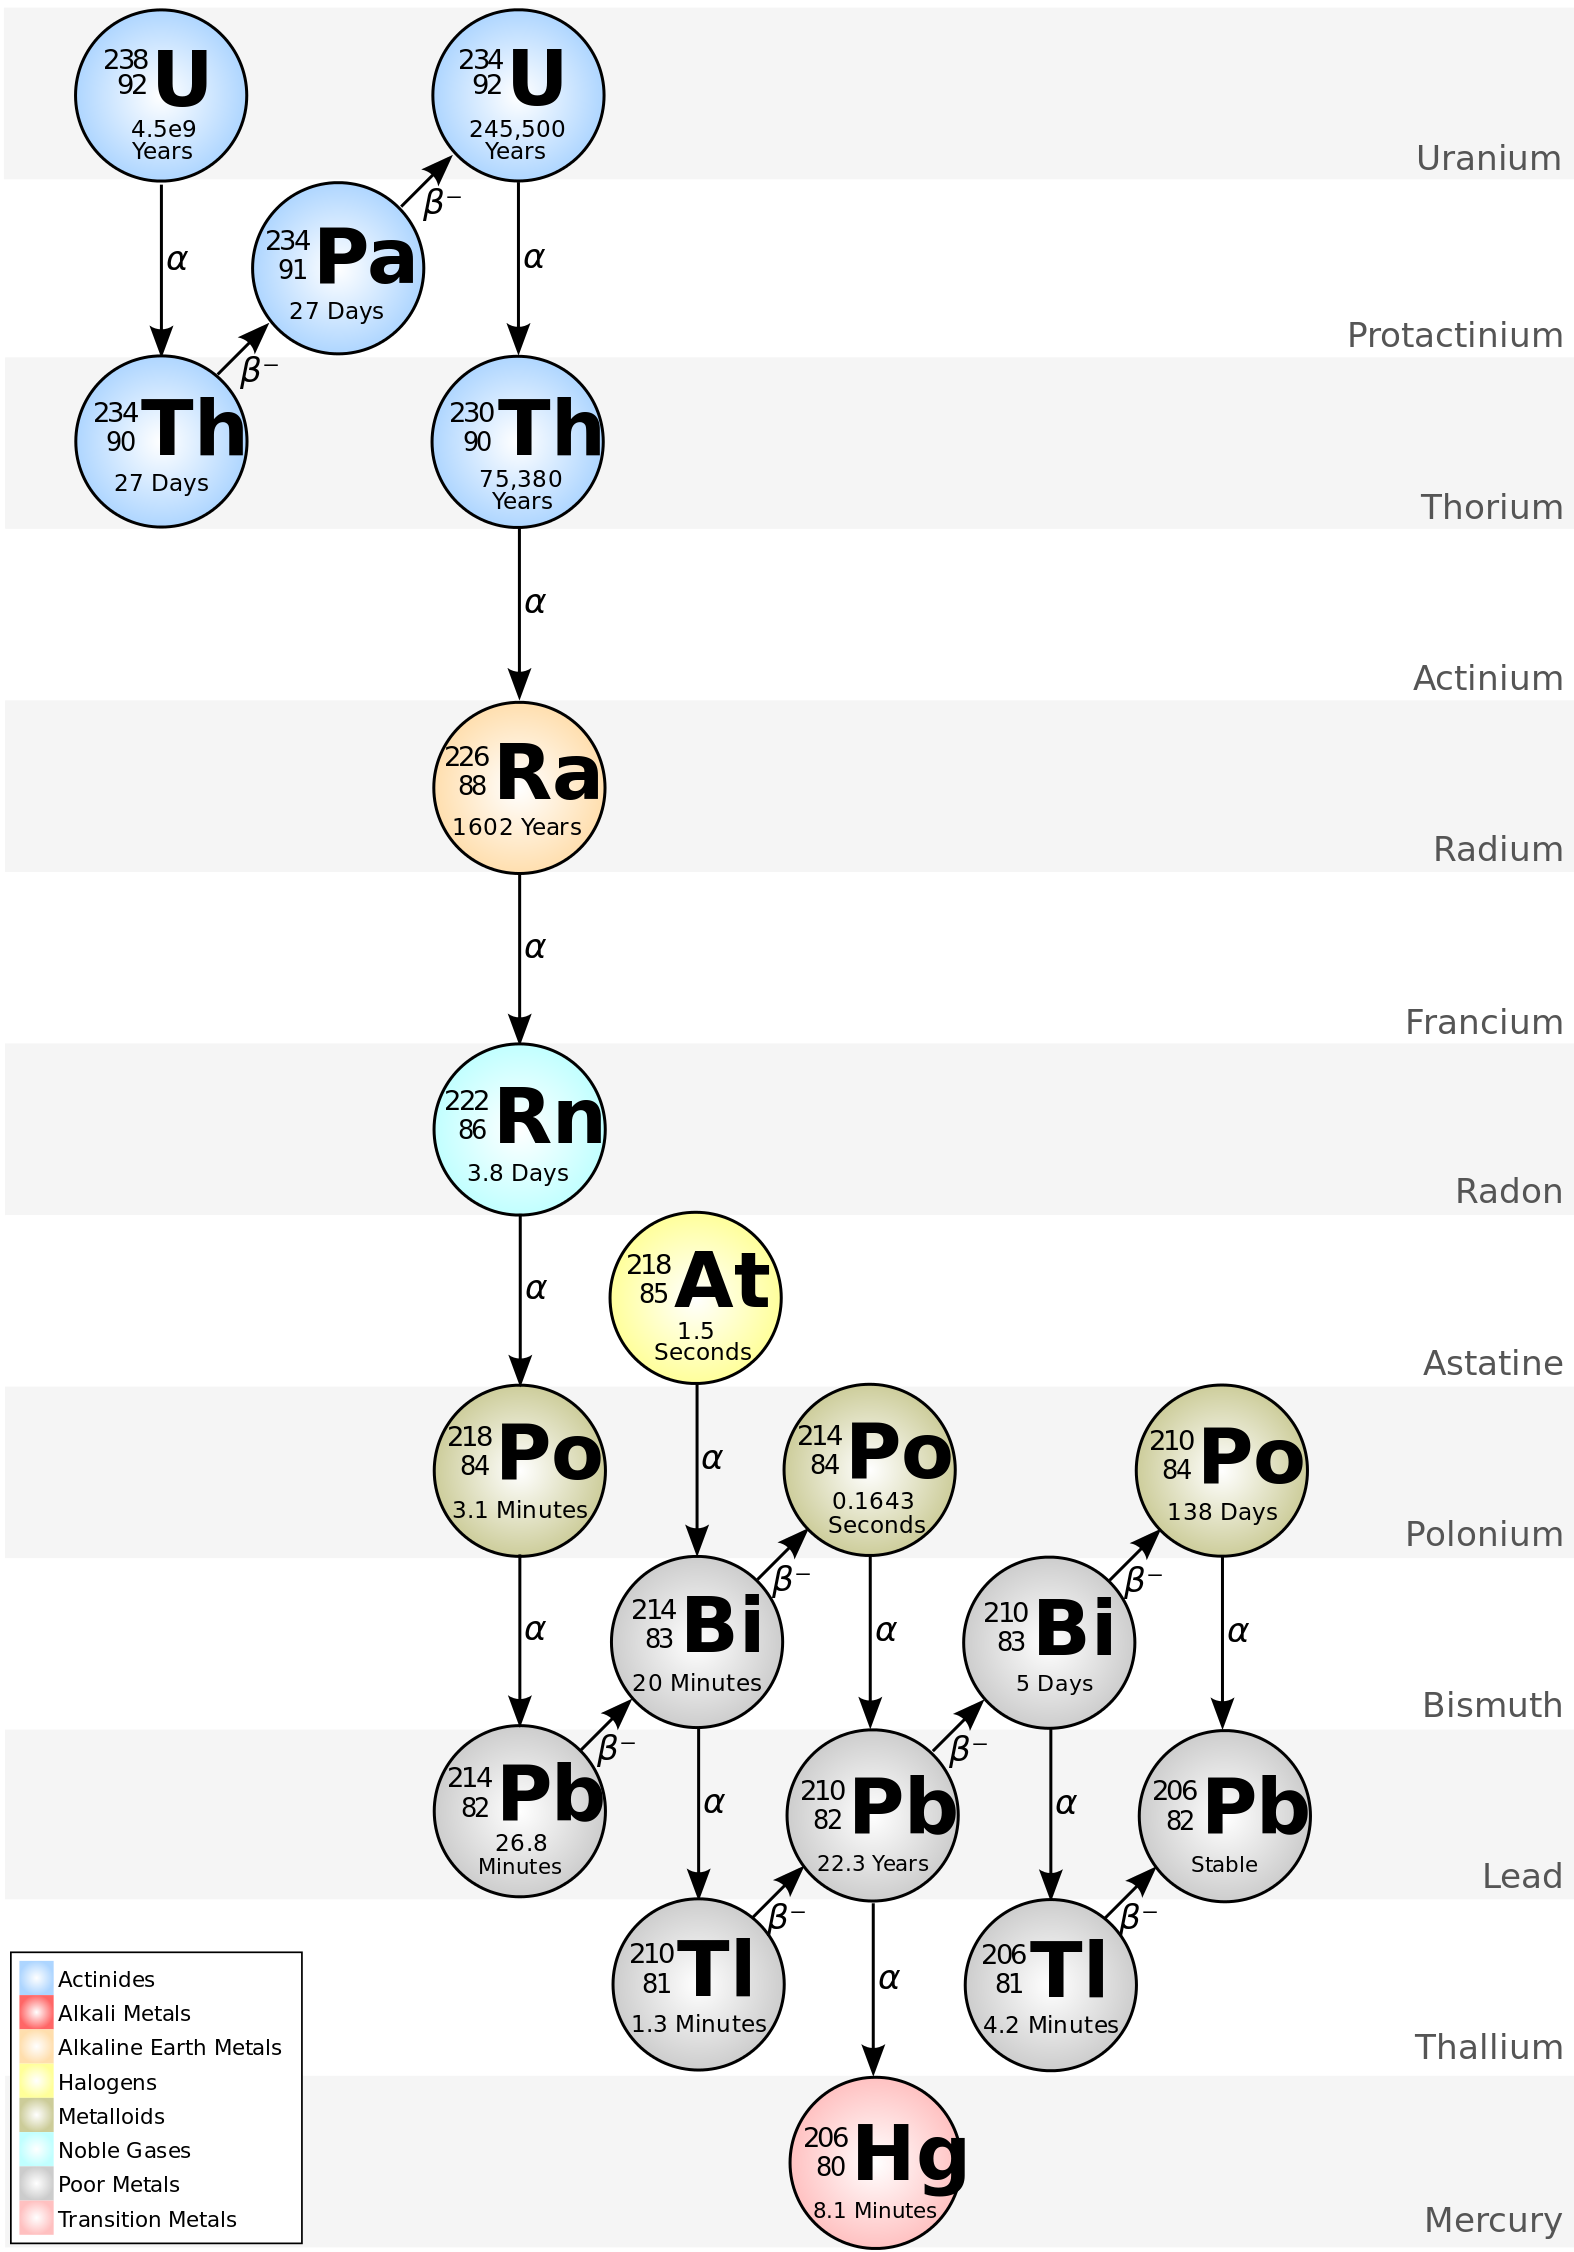
\includegraphics[width=0.5275\textwidth]{u238_chain}} \hfill
	\subfloat{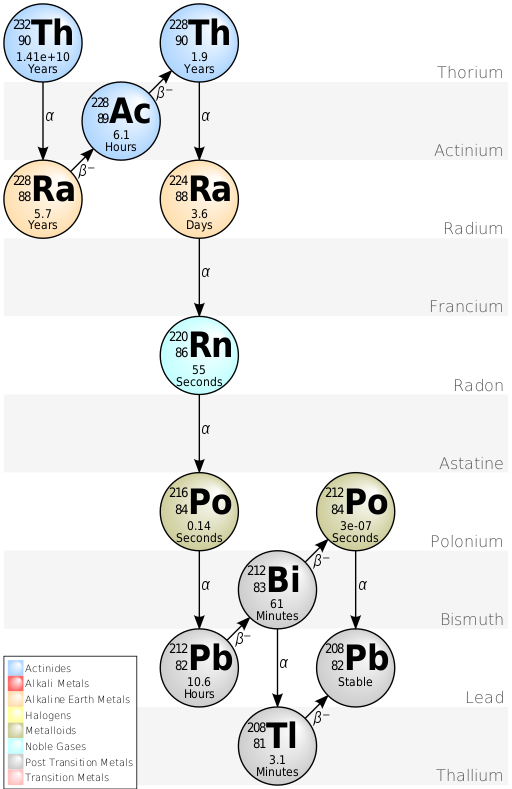
\includegraphics[width=0.4725\textwidth]{th232_chain}}
	\caption{The \uranium{} (left) and \thorium{} (right) decay chains.  The \uranium{} chain ultimately produces an intrinsic and the largest background source of electronic recoils in XENON1T while the \thorium{} chain results in a very useful electronic recoil calibration source.  Image Credit: Berkely Nuclear Forensics Group.}
	\label{fig:xe1t_rn_decay_chains}
\end{figure}


\subsubsection{\krypton{}}
\label{sec:xe1t_er_kr85}

\krypton{} is the other major internal source of background in liquid xenon based experiments.  While \krypton{} has a short half-life on a terrestrial scale (10.8 years), it is produced as the byproduct of nuclear fuel reprocessing and weapons tests.  \krypton{} $\beta$ decays with a maximum energy 687 keV with the spectrum decreasing steadily down to zero energy (as seen in \figref{fig:kr85_beta_decay}).  Commercial xenon will retain ppm to ppb levels of natural krypton (which contains \krypton{} at $2 \cdot 10^{-11}$ levels \cite{du2004atom}) as a result of the distillation process used to extract the xenon.  Due to its decay energy spectra, which allows for low energy electronic recoils, and relatively long half-life, which allows the \krypton{} due to disperse uniformly in the detector, \krypton{} is also considered to be one of the most dangerous backgrounds in XENON1T.  

Of course, ideally one would like to lower the krypton to xenon levels to as low levels as possible but the design goal of XENON1T was 0.2 ppt which translates to approximately 30 low energy electronic recoils per year in a 1 ton fiducial volume.  Using the krypton distillation column discussed in \secref{sec:xe1t_pur_kr85}, krypton to xenon levels of $0.36 \pm 0.06$ ppt were reached for the first science run putting XENON1T within a factor of two of the ultimate goal \cite{aprile2017xenon1t}.


\subsubsection{Solar Neutrinos}
\label{sec:xe1t_er_bkg_neutrinos}

Due to the mass difference between electrons and nucleons, significantly lower energy neutrinos are required for electronic recoils versus nuclear recoils.  This implies neutrinos from the sun, \textit{solar neutrinos}, will be the dominant source of neutrinos for electronic recoil background.  The energy spectra of solar neutrinos is shown in \figref{fig:solar_neutrino_flux}.  

Like electronic recoils from beta decays, the kinetic energy of the recoiling electron will follow a spectrum where only very low energies are relevant.  Unlike most of the other sources of electronic recoils, the solar neutrino background cannot be reduced and will scale with the size of the detector used.


\subsubsection{\radioxenon}

One source of background that has been mentioned in passing is the only radioisotope of natural xenon, \radioxenon{}.  \radioxenon{} was shown to decay via a \doublebeta{} decay with a half-life of $2.2 \cdot 10^{21}$ y \cite{barros2014double}.  The \doublebeta{} decay energy spectrum from \radioxenon{} is shown in \figref{fig:xe1t_er_bkg_all} and \figref{fig:xe1t_er_bkg_low} -- fortunately, unlike the beta decays resulting from the \radon{} chain and \krypton{} decay, the spectrum of \radioxenon{} decreases rapidly as electron momentum approaches zero \cite{ponkratenko2000event}.

While at the current sizes of xenon detectors this background is subdominant, it will eventually become a large source of irreducible background. 

% since radon and krypton dominated sr0 used a flat background spectrum in energy ROI

\subsection{Nuclear Recoil Background in XENON1T}
\label{sec:xe1t_nr_bkg}

Since WIMPs are expected to interact with xenon via nuclear recoils, any source of background that could cause a nuclear recoil in xenon is particularly troubling.  Care must be taken to make sure that all potenital sources of nuclear recoils are understood and accounted for --- otherwise an experiment would be susceptible to artificially strong limits or potential false discoveries.

The three major sources of nuclear recoil background are the detector materials themselves, which was discussed in \secref{sec:xe1t_materials_bkg}, neutrinos, and neutrons produced by high energy muons.  Each of these sources of background is shown in the full nuclear recoil background energy spectrum found in \figref{fig:xe1t_nr_bkg}.  

\begin{figure}[t]
	\centering
	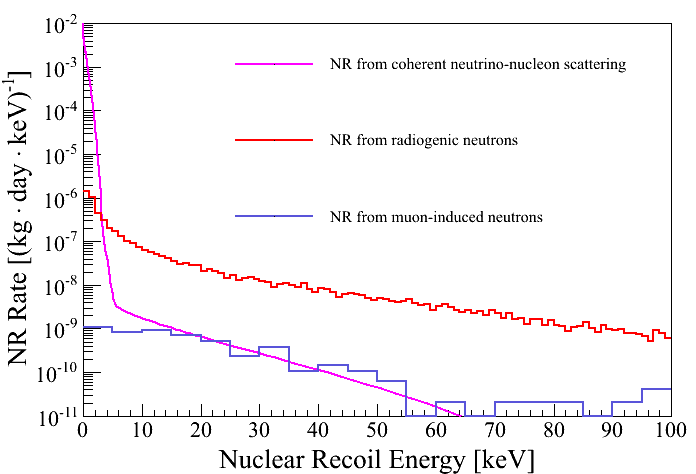
\includegraphics[width=0.95\textwidth]{xe1t_low_energy_nr_bkg}
	\caption{The energy spectra of the different sources of nuclear recoil background.  Image Credit: \citeref{aprile2016physics}.}
	\label{fig:xe1t_nr_bkg}
\end{figure}



\subsubsection{Coherent Neutrino-Nucleon Scattering}

Neutrinos can interact with both electrons, as discussed in \secref{sec:lxe_er} and \secref{sec:xe1t_er_bkg_neutrinos}, and atomic nuclei, via coherent neutrino-nucleon scattering (CNNS).  The maximum energy of a recoiling nucleus is given by $E_{\textrm{r}}^{\textrm{max}} = \frac{2 E_{\nu}^2}{m_N + 2 E_{\nu}}$, where $m_N$ is the mass of the nucleus and $E_{\nu}$ is the energy of the neutrino.  This implies that neutrinos must have energies on the order of 10 MeV to cause nuclear recoils on the order of 1 keV.  Therefore, high energy neutrino sources like \ce{^{8}B} in the sun as well as neutrinos from supernovae and the atmosphere will contribute the most to the CNNS background in dark matter experiments.

Unlike radiogenic nuclear recoils from radiogenic neutrons and muon-induced neutrons, this background cannot be shielded and cannot be reduced, in any reasonable sense, by a fiducial volume cut.  Therefore, as dark matter detectors become more and more sensitive this will constitute an irreducible background.

\subsubsection{Nuclear Recoils from muon-induced neutrons}

We discussed the possibility of a neutron background as the result of high-energy cosmogenic muons interacting in the rock and concrete surrounding the laboratory and the detector in \secref{sec:muon_veto}.  Given the efficiency of the muon veto and the low flux of muons expected because of the rock above the laboratory, the expected rate of nuclear recoils from muon-induced neutrinos is extremely low, as can be seen in \figref{fig:xe1t_nr_bkg}.



\section{The Calibration and Characterization of XENON1T for the First Science Run}
\label{sec:xe1t_calibrations}

In this section we will discuss the most important calibrations needed for the first science run of XENON1T.  We will also briefly discuss the basic cuts made during the first science run and their acceptance.  All of these cuts and calibrations are necessary for the discussions of the following two sessions regarding the calibration of XENON1T to nuclear recoils (performed by the author) and the first dark matter search.


% SPE
% position correction

\subsection{PMT Characterization}
\label{sec:xe1t_pmt}

One of the most basic tasks in TPCs of any size is to characterize the response of PMTs (\secref{sec:photomultiplier_tubes}) to photons that create a single photoelectron (SPE).  While the ideal case is that we completely understand the shape of the response function of the PMT (essentially the probability distribution function of how large the output signal will be given a single photoelectron), most experiments settle for understanding only the mean and variance of the distribution.  The reason for this practical compromise is that the single photoelectron response of a PMT is roughly normal and that when dealing with a large number of photoelectrons ($\gtrapprox 20$ PE), by the central limit theorem, the response will appear to be a normal distribution defined by only the mean and the variance of the single photoelectron response.  Therefore, an understanding of the full photoelectron response will never be necessary for S2s, even for the smallest signals.  However, a full understanding of the response of a PMT to a single photoelectron could be beneficial in understanding very small S1 signals.

Two methods were used to characterize the response of the PMTs for XENON1T during the first science run.  Both involved using low levels of blue light to illuminate the PMTs such that the probability distribution of photons detected is approximately Possonian.  The first method involves assuming a distribution for the background distribution (no light detected) and the SPE response and using these assumptions to fit the low light spectrum.  In XENON1T, it was assumed that the background distribution is Gaussian with an exponential component and that the single photoelectron response, before convolution with the background, is Gaussian.  A sample fit with the labeled components is shown in \figref{fig:xe1t_spe_gaussian}.



\begin{figure}[t]
	\centering
	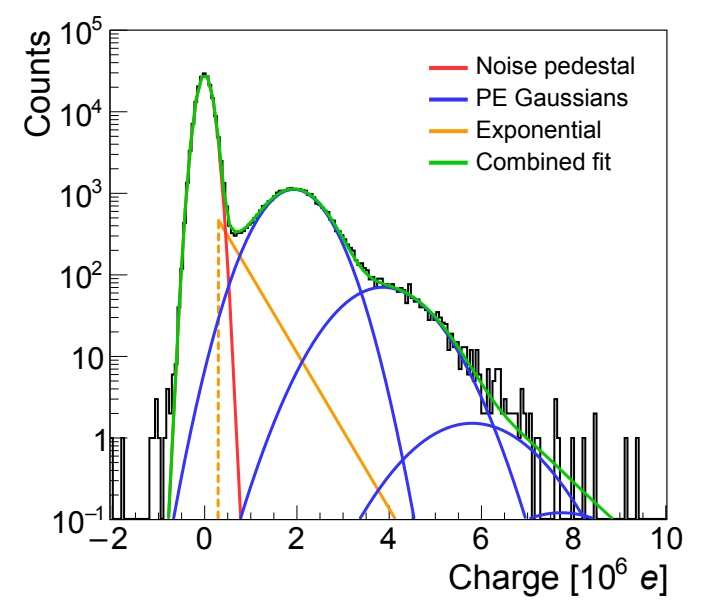
\includegraphics[width=0.8\textwidth]{xe1t_spe_gaussian}
	\caption{A fit of the low light response of one of the XENON1T PMTs in order to characterize the single photoelectron response.  Image Credit: \citeref{barrow2017qualification}.}
	\label{fig:xe1t_spe_gaussian}
\end{figure}


The second method used to calibrate the charge response of single photoelectrons in a completely statistical and model-independent way.  While this method requires a background measurement that is completely compatible with the measurement at low light levels (for example, the electronics of the light source causing additional background would be an example of incompatability), one can extract the mean and variance of the single photoelectron response very easily and without assumptions \cite{saldanha2017model}.

PMT characterization will be discussed in further detail in \appref{app:pmts} where we will describe a method that the author developed for the non-analytical characterization of PMTs using the cascade model.




\subsection{Position Reconstruction}
\label{sec:xe1t_pos_rec}

It has been mentioned several times that TPCs have the unique capability of reconstructing the three-dimensional position of an interaction within a detector.  We will now discuss how the interaction vertex was found during the first science run of XENON1T.

As was discussed in \secref{sec:xe_pos_rec}, in a dense medium such as xenon with a large uniform electric field across it, one would expect that free electrons are quickly accelerated to their drift velocity and stay at this velocity until reaching the liquid-gas interface.  Therefore, if one knows the drift velocity at the given electric field then one can measure the depth of the event from the drift time (very closely estimated by the time difference between the S1 and S2 of a given event).  Measuring the drift velocity is very simple --- the distance between the cathode and the gate (which is just below the liquid-gas interface) is known so by looking at the maximum drift time (the time it takes to travel from the cathode to the gate) one can approximate the drift velocity at the given field.  The maximum drift time can be found using a spectrum like the one shown in \figref{fig:xe1t_drift_time_vs_width}.  For the first science run of XENON1T, the maximum drift time to cover the 96.9 cm at approximately 12 \sfrac{kV}{cm} was 673 $\mu$s which gives a drift velocity of 1.43 \sfrac{mm}{$\mu$s}.


\begin{figure}[t]
	\centering
	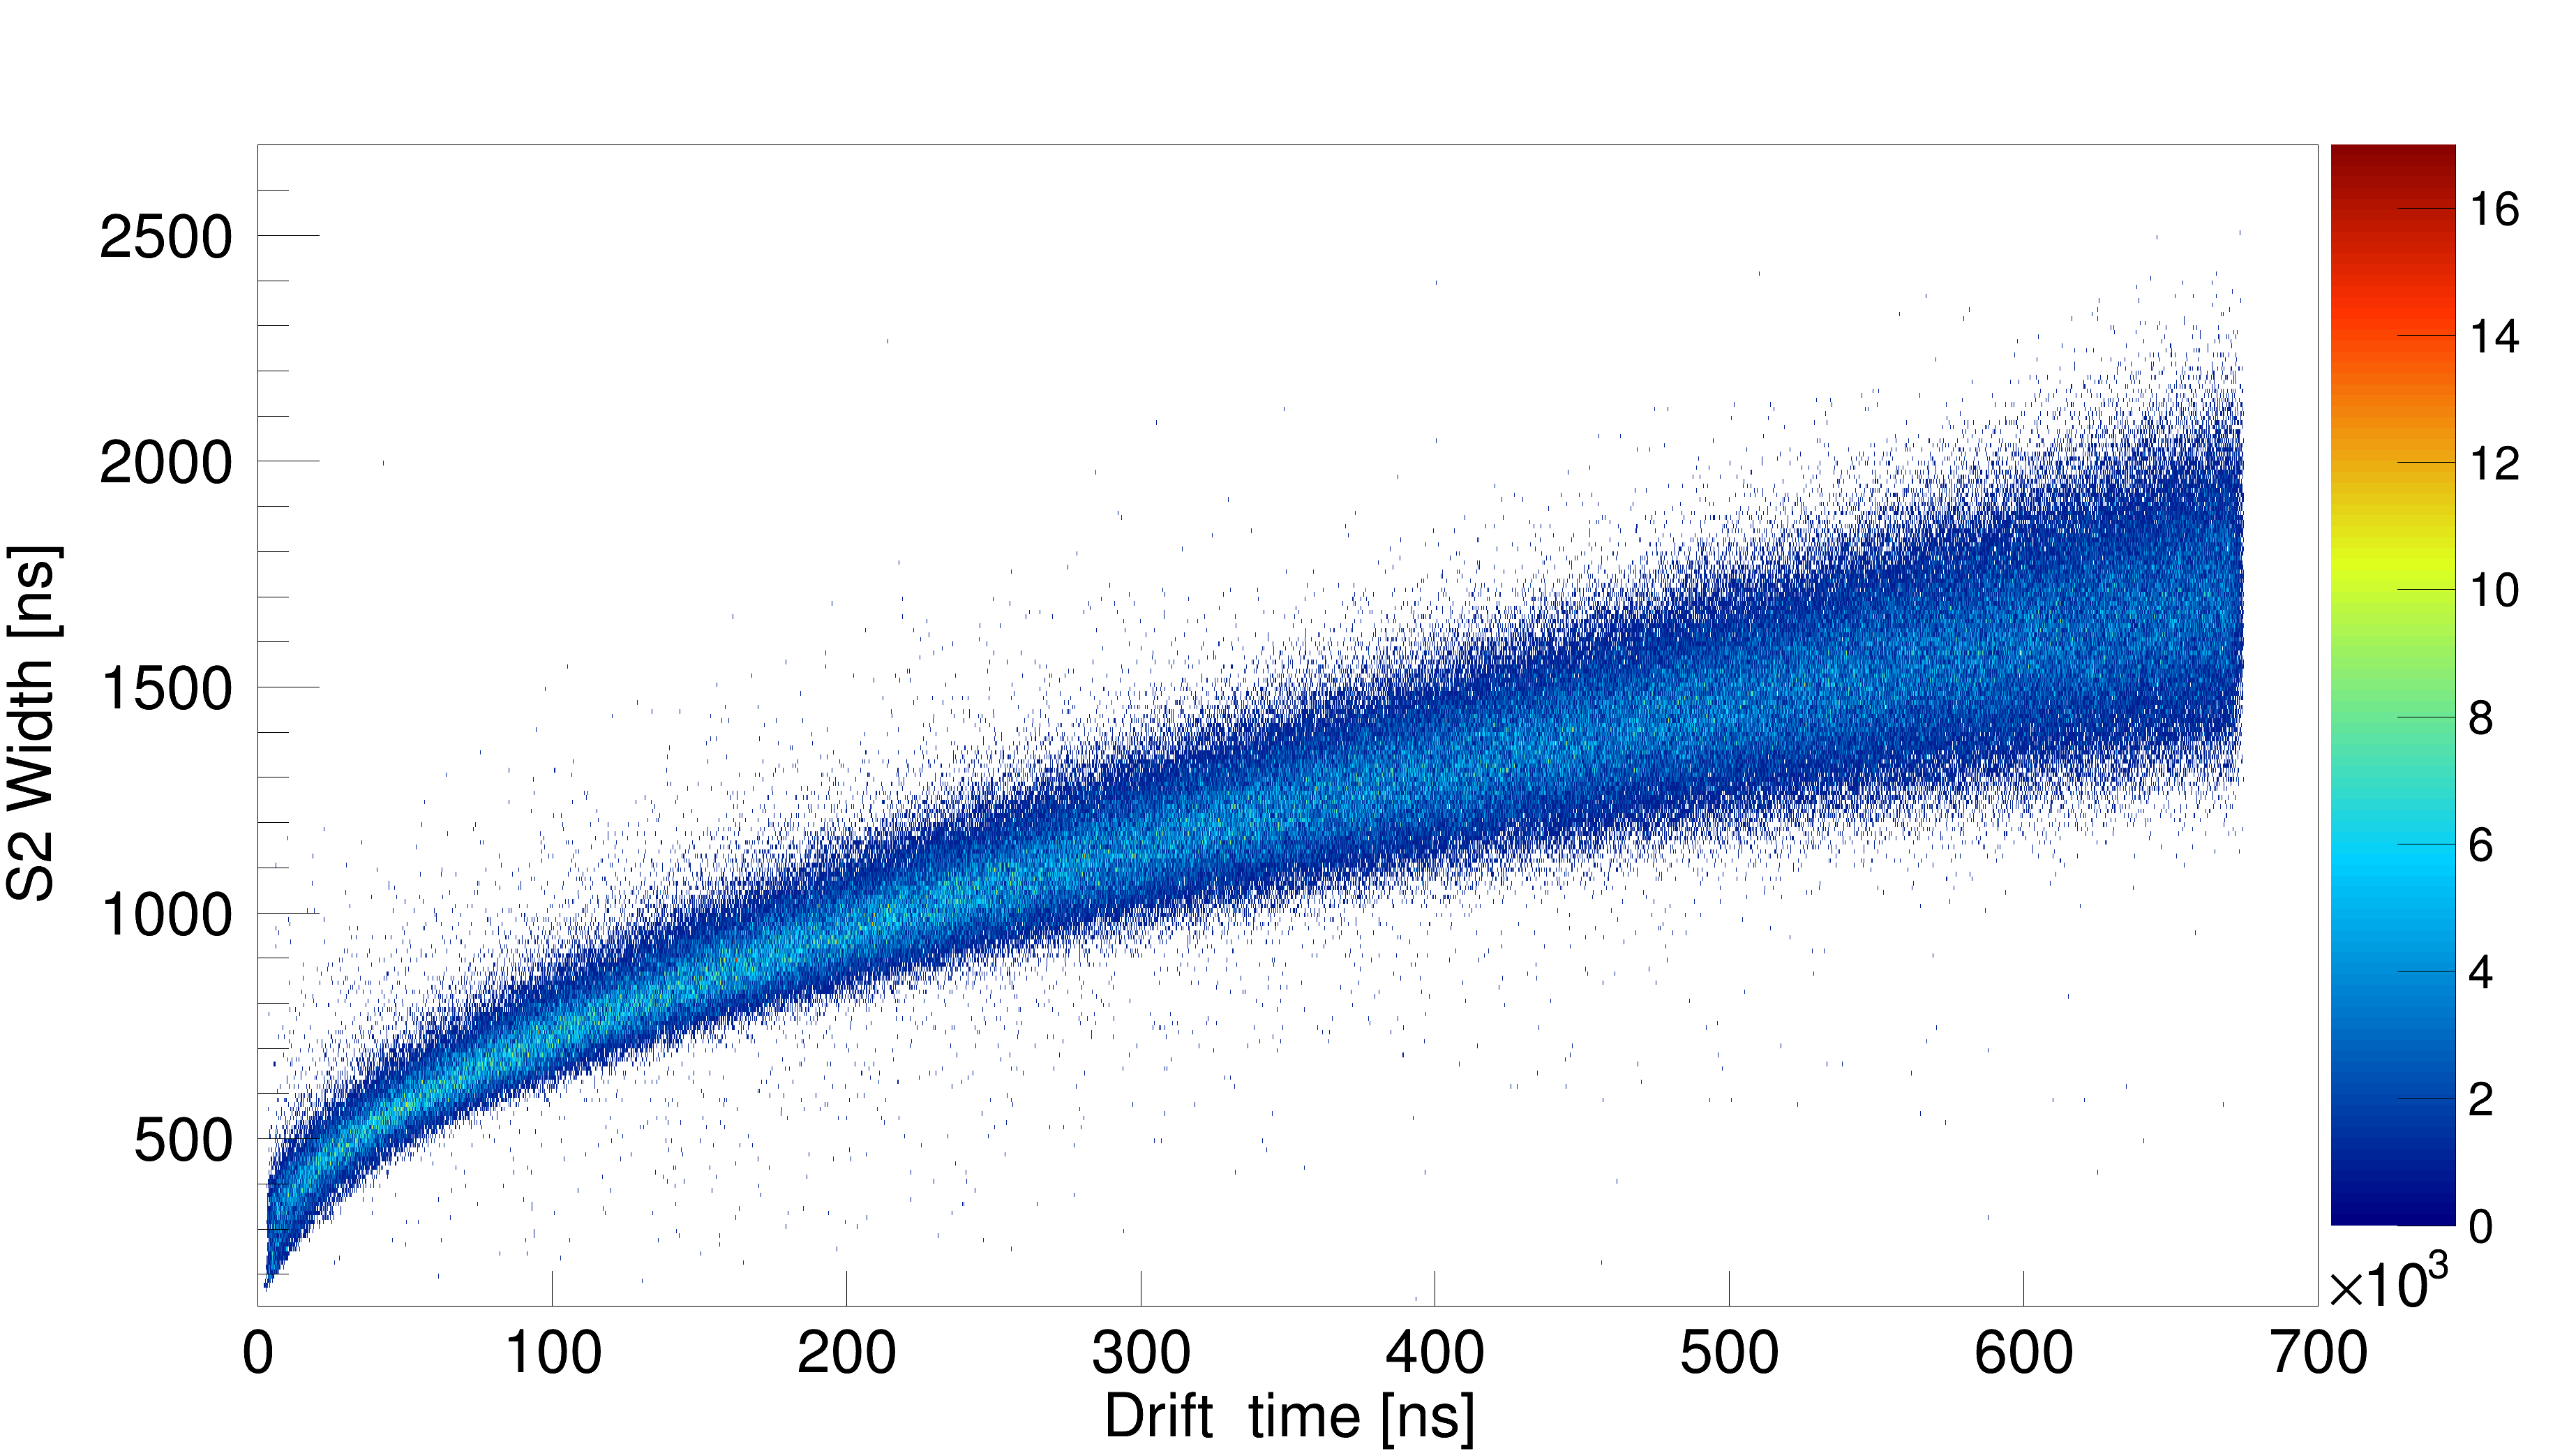
\includegraphics[width=0.99\textwidth]{xe1t_drift_time_vs_width}
	\caption{A plot of the width of an S2 versus the drift time for 32 keV events from \ce{^{83m}Kr}.  Note that at a certain drift time, no more events are seen.  This cut-off in events represents the location of the cathode since interactions below it will not produce an S2.}
	\label{fig:xe1t_drift_time_vs_width}
\end{figure}


Finding the location of electron extraction (a good proxy for the position given the field uniformity in the detector) for an event can be done by looking at the light pattern resulting from a given S2.  While this might seem relatively simple, consistently reconstructing the position within 2 cm of its actual location is a very complicated task due to detector effects.  Current methods of position reconstruction are reliant on simulation to produce either training data for a neural network or light collection efficiency maps for each of the top PMTs.  

While using multiple algorithms for position reconstruction is useful for consistency checks, ultimately only one algorithm can be used.  In the first science run of XENON1T, the algorithm used the simulated light collection efficiency maps for each PMT as part of likelihood function to find the position in the highest agreement with the measured pattern.  This method resulted in a less than 2 cm mean reconstruction error for simulated data with a signal size above the trigger threshold.  This error continuously decreases as the size of the S2 signal increases.  The more important test, though, is how the algorithm reconstructed the position of real events in the detector.  While we cannot compare positions event-by-event, we can look at the overall distribution of positions for a given source and compare that to our expectations.  \figref{fig:xe1t_pos_rec_kr} shows the distribution of positions in all dimensions for 32 keV events from \ce{^{83m}Kr}, which should be uniformly distributed inside of the detector.


\begin{figure}[t]
	\centering
	\subfloat{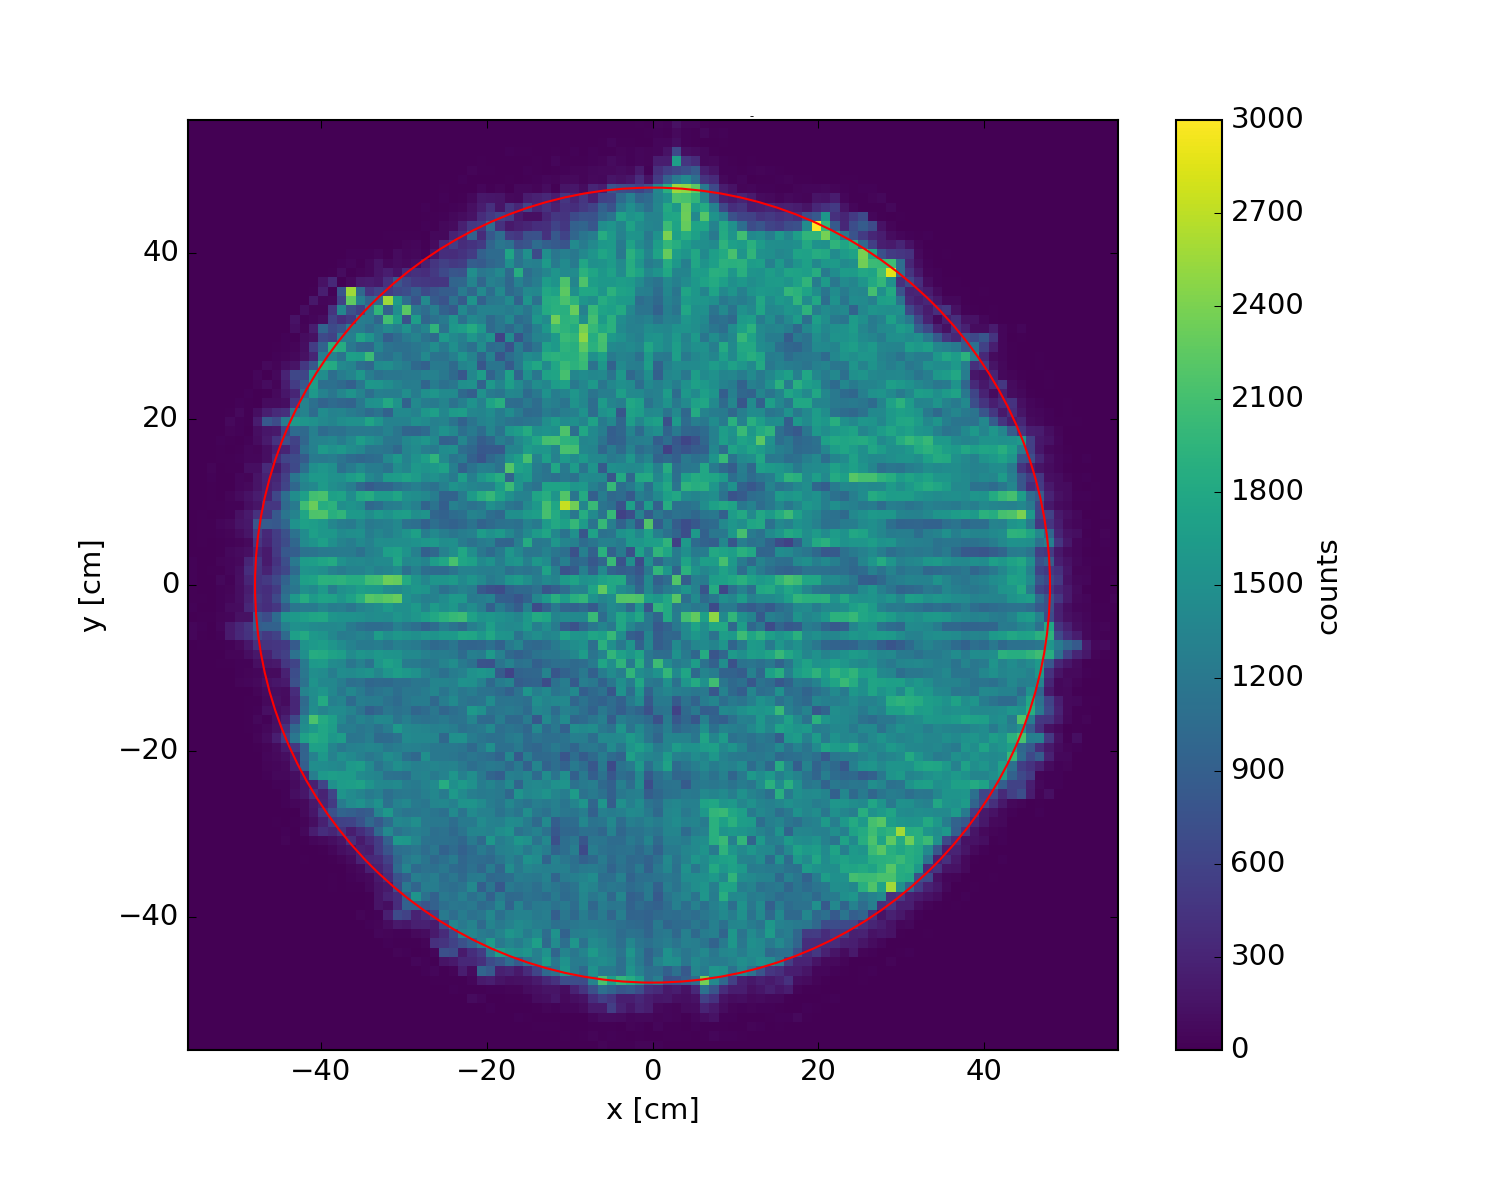
\includegraphics[width=0.555\textwidth]{xe1t_pos_rec_xy_kr}} \hfill
	\subfloat{\includegraphics[width=0.445\textwidth]{xe1t_pos_rec_zr2_kr}}
	\caption{The distribution of positions of 32 keV events from \ce{^{83m}Kr} during the first science run of XENON1T.}
	\label{fig:xe1t_pos_rec_kr}
\end{figure}


\subsection{Position Dependent Corrections}
\label{sec:xe1t_pos_dependent_corrections}

\subsubsection{S1 Position Correction}
\label{sec:xe1t_lce_pos_correction}

One subtle, but critical, detector effect is the fact that the position of an event will affect the size of the S1 seen.  Understanding these losses as a function of position are critical to improve the resolution of the detector.  Fortunately, this S1 position dependence can be measured in a very simple way.  By introducing a source that will distribute throughout the entire detector and give a monoenergetic recoil, we can measure the difference in light yield for given positions.  Uniform sources are very useful this type of measurement but they are not necessary, especially for small detectors.

In XENON1T, the 32 keV emission of \ce{^{83m}Kr} was used to find the S1 correction map, which is shown in \figref{fig:xe1t_s1_correction_map}.  The decay of \ce{^{83m}Kr} not only creates a 32 keV electronic recoil but actually is followed by a second decay with a lifetime of 154 ns and energy of 9.4 keV.  This close time coincidence can be used to further confirm that only 32 keV events are being kept for the analysis.  This correction map, which shows the light yield at a given position relative to the average light yield in the detector, can then be used to correct recoils of all energies and types to improve the detector resolution.  While the correction map could be in three dimensions, since the TPC is cylindrically symmetric, we only correct in radial and depth coordinates.


\begin{figure}[t]
	\centering
	\includegraphics[width=0.99\textwidth]{xe1t_s1_correction_map}
	\caption{The S1 correction map of XENON1T.  This correction map shows the relative light yield of events at specific positions relative to the average light yield of the detector for monoenergetic events.  One can see the clear trend that events closer to the bottom PMT array have higher light yields than those closer to the liquid-gas interface.}
	\label{fig:xe1t_s1_correction_map}
\end{figure}


A clear trend can be seen in \figref{fig:xe1t_s1_correction_map}: the closer to the bottom PMT array an event is, the higher the light yield will be.  To a lesser extent, the closer the event is to the center of the detector, the higher the light yield will be.  This trend is related to the longer path length and larger number of reflections events towards the top and edge of the detector will have versus events very close to the bottom PMT array.

In theory, the position dependence of S1 could also be simulated but given the many factors that need to be understood and fed into the simulation, such as the absorption length and the Rayleigh scattering length in liquid xenon for 178 nm photons in liquid xenon, the reflectivity of the different materials, and the optical transparency of the meshes, this is impractical (especially given the simplicity of a direct measurement.


\subsubsection{S2 Transverse Position Correction}

In almost the same way that we can find the S1 correction map, we find S2 transverse position correction map.  However, instead of only using the 32 keV signal, we used the S2 of both the 32 keV and 9 keV decays (since they can only be resolved in S1 and not S2).  The correction maps for the top and bottom PMT arrays are shown in \figref{fig:xe1t_s2_correction_map_xy}.


\begin{figure}[t]
	\centering
	\subfloat{\includegraphics[width=0.5\textwidth]{xe1t_s2_correction_map_xy_top}} \hfill
	\subfloat{\includegraphics[width=0.5\textwidth]{xe1t_s2_correction_map_xy_bottom}}
	\caption{The S2 transverse position correction map of XENON1T.  This correction map shows the relative charge yield of events at specific positions relative to the average charge yield of the detector for monoenergetic events.  One can see the trend for the bottom PMT array that events closer to the center of the detector have higher charge yields than events closer to the edges.}
	\label{fig:xe1t_s2_correction_map_xy}
\end{figure}

As one can see, the correction maps look quite different.  This is mainly due to the close proximity of the S2 light to the top PMT array such that non-functional PMTs cause features in the map.  The S2 transverse position correction map for the bottom PMT array, on the other hand, is very smooth because the light must travel further and is less dependent on single PMT.  Ultimately, in the first science run, it was decided that only the bottom PMT array would be used for calculating signal sizes so only the smoother bottom PMT map was needed.

In the bottom PMT map, one can again see the trend that events towards the center of the detector have higher charge yields than events closer to the edge of the TPC.  This effect is believed to be from charge collecting on the teflon, edge effects for the electric field produced by the anode and the gate, and again from the longer path lengths and larger number of reflections for photons originating closer to the edge of the detector.


\subsubsection{S2 Depth Correction Correction: Electron Lifetime}

As mentioned in \secref{sec:tpc_s2_sig}, the free electrons extracted from the interaction site by the drift field can be absorbed by electronegative impurities contaminating the liquid xenon.  These impurities, mostly oxygen, will therefore decrease the size of the S2 signal measured.  It turns out that the probability that an electron successfully reaches the liquid-gas interface is well described by the fairly simply relationship shown in \eqnref{eqn:xe1t_electron_lifetime}.

\begin{equation}
        \label{eqn:xe1t_electron_lifetime}
        p_{\textrm{EL}}(z) = \frac{1}{\tau_{e^-}} e^{-\frac{z}{v_d \tau_{e}}}
\end{equation} 

Since the S2 signal size is directly proportional to the number of electrons accelerated through the gaseous xenon, \eqnref{eqn:xe1t_electron_lifetime} should manifest itself as an exponential decrease in the S2 size as a function of depth.  A plot of this effect can be seen in \figref{fig:xe1t_electron_lifetime}.


\begin{figure}[p]
	\centering
	\includegraphics[width=0.99\textwidth]{../../Chapter2/images/tpc_electron_lifetime.jpeg}
	\caption{An example of an electron lifetime analysis from XENON1T.  In this analysis, the 41 keV \ce{^{83m}Kr} electronic recoil is used and the decay's S2 signal size is plotted versus drift time (a proxy for depth).  Image Credit: \citeref{aprile2017xenon1t}.}
	\label{fig:xe1t_electron_lifetime}
	
	\centering
	\includegraphics[width=0.99\textwidth]{xe1t_electron_lifetime_sr0}
	\caption{The electron lifetime over the course of the first science run of XENON1T.  Notice the two drops in the electron lifetime corresponding to periods when the purification system was not operating.  Shown in red is a prediction of the electron lifetime given the detector operating parameters and outgassing estimates from materials.  Image Credit: \citeref{aprile2017xenon1t}.}
	\label{fig:xe1t_electron_lifetime_sr0}
\end{figure}


Electronegative impurities emanate from the materials used to construct the detector and therefore are constantly introduced into the system.  Therefore, these impurities must constantly be cleaned out.  This cleaning also does not remove all impurities instantaneously --- the electron lifetime must be measured routinely in order to monitor its day-to-day changes.  These effects can be seen in \figref{fig:xe1t_electron_lifetime_sr0} which shows both drops from when the purification went offline and the steady increase in purity from continuous cleaning.


In XENON1T, this cleaning is done by the purification system described in \secref{sec:xe1t_pur_electronegative}.  Because the a low electron lifetime has an adverse impact on the S2 resolution (and hence energy resolution and discrimination power), significant effort has gone into and will continue to go into improving electronegative purification for large scale detectors.  


\subsection{Single Electron Gain}
\label{sec:xe1t_gas_gain}

The single electron gain, also referred to as \textit{gas gain}, is used to quantify the number of photons detected per electron extracted from the liquid into the gas phase.  While both the production of scintillation light from electrons exciting gaseous xenon atoms and the detection of scintillation photons are both well approximated by Poisson processes.  However, due to detector effects, such as the per PMT detection efficiency and variations in the field in the gaseous xenon, will cause further smearing of the number of photons detected from a single electron.  If we assume that this smearing is Gaussian, then we can actually fit the number of photons detected with a Poisson convolved with a Gaussian to determine the final probability mass function.  

An example of a fit of the gas gain is shown in \figref{fig:xe1t_single_electron_gain} where hits are found by looking at voltage excursions over threshold on a per-PMT basis in a time window defined by the waveform summed across all PMTs.

\begin{figure}[t]
	\centering
	\includegraphics[width=0.99\textwidth]{xe1t_single_electron_gain}
	\caption{The fit single electron gain from the first science run of XENON1T.  Hits are defined as excursions above threshold for individual PMTs in a time window defined by the waveform summed across all PMTs.}
	\label{fig:xe1t_single_electron_gain}
\end{figure}


Since it is expected that the gas gain is sensitive to the electric field in the gas phase, the gas gain is susceptible to change with small changes in the liquid level.  Therefore, the gas gain is constantly monitored throughout data taking to ensure that it is stable.


\subsection{Average Light Collection Efficiency and Extraction Efficiency}
\label{sec:xe1t_anticorrelation}


In \secref{sec:lxe_er_observables}, we discussed the observables production process for electronic recoils and found a relationship between the energy of electron recoils and the number of photons and free electrons produced because of the lack of quenching factors in the observables production mechanism.  This relationship is shown in \eqnref{eqn:xe1t_anticorrelation} where $N_q$ is the number of quanta, $\textrm{E}_{\textrm{ER}}$ is the energy of the electronic recoil, $W$ is the average energy required to produce an exciton or electron-ion pair ($13.7 \pm 0.2$ eV \cite{dahl_thesis}), $N_{\gamma}$ is the number of photons produced in the electronic recoil, and $N_e$ is the number of free electrons extracted from the interaction site.

\begin{equation}
        \label{eqn:xe1t_anticorrelation}
        N_q = \frac{\textrm{E}_{\textrm{ER}}}{W} = N_{\gamma} + N_{e}
\end{equation}

While \eqnref{eqn:xe1t_anticorrelation} looks very simple, it actually proves to be very valuable when measuring two otherwise very difficult to measure/simulate detector parameters: the average light collection efficiency of photons and the extraction efficiency of electrons from the liquid into the gas.  

We can easily convert the number of photons and free electrons from the interaction into the observables measured by our detector, S1 and S2.  Since S1 is the number of photons detected, we say that $\textrm{S1} = N_{\gamma} \cdot g_1$, where $g_1$ is the average light collection efficiency.  The S2 signal is directly proportional to the number of electrons extracted from the liquid into the gaseous xenon.  Therefore, we can say that $\textrm{S2} = N_e g_2 = N_e \cdot G_e \eta$ where $G_e$ is the single electron gain (see \secref{sec:xe1t_gas_gain}) and $\eta$ is the efficiency of extracting electrons from the liquid into the gaseous xenon (often referred to as the \textit{extraction efficiency}).

  This allows us to put \eqnref{eqn:xe1t_anticorrelation} into terms of measured parameters.
  
\begin{equation}
        \label{eqn:xe1t_anticorrelation_s1_s2}
        \frac{\textrm{E}_{\textrm{ER}}}{W} = \frac{\textrm{S1}}{g_1} + \frac{\textrm{S2}}{G_e \eta}
\end{equation}
 
  \begin{figure}[t]
	\centering
	\includegraphics[width=0.95\textwidth]{xe1t_doke_plot}
	\caption{The Doke plot for XENON1T along with the best fit.  Note that only the bottom PMT array is used for the S2 signal and that we use the position corrected values of S1 and S2.  While the de-excitation from neutron captures in water is shown (\ce{^{2}H} with an de-excitation energy of 2.225 MeV), it is not used for the fit.}
	\label{fig:xe1t_doke_plot}
\end{figure}

 
We can now look at multiple monoenergetic peaks or the same monoenergetic peak at different electric fields (or multiple monoenergetic peaks at multiple electric fields).  A simple rearrangement of \eqnref{eqn:xe1t_anticorrelation_s1_s2} shows us that the S1 and S2 values of these peaks should fall along a line defined by $g_1$, $\eta$, and $G_e$.

 \begin{equation}
        \label{eqn:xe1t_anticorrelation_line}
        \frac{\textrm{S2}}{\textrm{E}_{\textrm{ER}}} = \frac{G_e \eta}{g_1} \frac{\textrm{S1}}{\textrm{E}_{\textrm{ER}}} - \frac{G_e \eta}{W}
\end{equation}
 
 We can fit what is colloquially referred to as a \textit{Doke plot} (after Tadayoshi Doke) with the mean S1 and S2s of various monoenergetic electronic recoils (potentially at different fields) using \eqnref{eqn:xe1t_anticorrelation_line} in order to extract $g_1$ and $eta$.  Note that $eta$ can only be extracted if one independently measures the single electron gain since otherwise the two parameters will be completely correlated.  The fit of multiple monoenergetic electronic recoils to find the extraction efficiency and the average light collection efficiency of XENON1T is shown in \figref{fig:xe1t_doke_plot}. 
 
 

\subsection{Cut Acceptance}
\label{sec:xe1t_cut_acceptance}

\begin{figure}[t]
	\centering
	\includegraphics[width=0.99\textwidth]{xe1t_cut_acceptances}
	\caption{The estimated cut acceptances in S1 and S2 for the first science run of XENON1T.}
	\label{fig:xe1t_cut_acceptances}
\end{figure}


Cuts in XENON1T are used to eliminate background sources, like the fiducial volume cut and the single scatter cuts, or to remove events that show non-standard behavior, such as the S2 width cut that uses the diffusion model to define appropriate widths given a drift time (this relationship between drift time and width can actually be seen in \figref{fig:xe1t_drift_time_vs_width}).  Once the cuts are in place, it is important to understand the population of good events that are removed as a function of signal size --- this is referred to as the \textit{cut acceptance}.  

To define the cut acceptance, we use the ``N-1'' approximation.  The N-1 approximation calls for applying all but a single one of the cuts to define the control sample which is then compared to the sample after applying the final cut.  It is important to note that this does not account for potential correlations between cuts.  Using the N-1 approximation for each of the cuts and combining the individual acceptances, we can find the overall cut acceptance of the first science run of XENON1T as a function of S1 and S2 (shown in \figref{fig:xe1t_cut_acceptances}).

It is important to note that, with a sufficiently trust-worthy physics and detector simulator, one could estimate the cut acceptances using simulation. 




\section{Electronic and Nuclear Recoil Characterization of XENON1T}
\label{sec:xe1t_er_nr_calibration}

The electronic and nuclear recoil calibrations are two of the most important studies required for a liquid xenon TPC.  For the first time in xenon detectors, these calibrations were performed such that a realistic approximation of the microphysics process was accounted for alongside the detector effects discussed.  This was only made possible with the use of a fast Monte Carlo (MC) framework that was developed by the author and discussed in \appref{app:gpus} that leveraged graphical processing units (GPUs) for dramatic increases in speed (two to three orders of magnitudes).

While these calibrations can (and in future science runs will be) performed together due to the large number of shared parameters, in the first science run of XENON1T they were performed separately.  


\subsection{Significance of the Calibrations}

Before discussing the details of the calibrations, it is helpful to understand why these calibrations are of such high importance.  Ultimately, the goal of each science run is to search for a WIMP signal in the detector.  While this can be done in a purely statistical fashion (as discussed in \secref{sec:dm_direct_detection}), more sophisticated methods have been developed that drastically improve the sensitivity of TPCs to WIMPs.  

Since the background in XENON1T is thoroughly understood, as outlined in \secref{sec:xe1t_er_bkg} and \secref{sec:xe1t_er_bkg}, we can actually create a probability distribution function (PDF) in our signal space (S1 and S2 space or some variation of this) \textit{if} our calibration captures the various processes between energy deposition all the way to signal extraction by the processor.  This probability distribution function can be made with WIMPs (or other dark matter candidates) to determine whether or not the data agrees with a WIMP of a given mass and cross section.  Determining how well WIMPs of given masses and cross sections agree with the data ultimately determines the limit set (if all WIMPs below a given cross section agree with the data) or whether a discovery was made (if the data favors a particular mass and cross section more than all others).

\begin{figure}
        \centering
	\includegraphics[width=0.99\textwidth]{xe1t_background_pdf}
	\caption{The probability distribution function for the first science run of XENON1T plotted with the cumulative density contours of a 50 $\sfrac{\textrm{GeV}}{\textrm{c}^2}$ WIMP.  The combined signal and  background PDF is used to either set a limit on the WIMP mass and cross section or claim a discovery.}
	\label{fig:xe1t_background_pdf}
\end{figure}

\figref{fig:xe1t_background_pdf} shows the PDF of the background distribution for the first science run with the cumulative density contours of a 50 $\sfrac{\textrm{GeV}}{\textrm{c}^2}$ WIMP.  These PDF and contours were made using the signal production models that were measured via the electronic and nuclear recoil calibrations.



\subsection{Parameter Estimation via Monte Carlo}


\begin{figure}
        \centering
	\includegraphics[width=0.99\textwidth]{xe1t_fast_mc_flowchart}
	\caption{A flowchart summarizing how a fast Monte Carlo is used to estimate the parameters in the signal production model.  Orange steps are done in each iteration of the parameter estimation where as black arrows represent steps that are only done a single time.}
	\label{fig:xe1t_fast_mc_flowchart}
\end{figure}


\figref{fig:xe1t_fast_mc_flowchart} shows a flowchart that summarizes how the calibration of electronic and nuclear recoils is performed.  The main idea is that a detailed Monte Carlo is used to estimate the expected distribution of events in signal space (S1 and S2 for XENON1T), which can then be compared to the actual measured distribution of events to determine what values for the parameter model cause the highest level of agreement. 

In more technical terms, the Monte Carlo is used to create a PDF which is then compared with data which results in a likelihood.  This likelihood can be combined with prior distributions of the model parameters (from previous measurements or calibrations).  As you vary the parameters in the signal production model, you would expect this likelihood to increase and decrease.  One can then use different algorithms to find either the set of parameters best in agreement with the data (via a minimizer) or the posterior distribution of the parameters (via a Markov Chain Monte Carlo or MCMC).

The benefit to using a Monte Carlo to define a likelihood for parameter estimation is that your signal production model can be arbitrarily complex.  The downside of using a MC to estimate your likelihood is that it is extremely inefficient, typically rendering this approach impractical.  However, using graphical processing units, the author was able to develop an analysis framework that made this type of analysis feasible.  The details of the framework will be discussed in detail in the \appref{app:gpus}.

The details of Monte Carlo event production will be discussed in \secref{sec:xe1t_mc_observables_production_er}, \secref{sec:xe1t_mc_observables_production_nr}, and \secref{sec:xe1t_mc_detector}.  These Monte Carlo events are used to fill a histogram that is compared with a histogram filled with data via a binned likelihood, which will be discussed in \secref{sec:xe1t_mc_likelihood}.  In this way we can quantify how well a given set of parameters agrees with what we have measured.  The set of parameters to be tested is chosen in this analysis by a Markov Chain Monte Carlo (MCMC) but realistically could be done with most parameter estimation algorithms --- we will briefly discuss how the posterior probability space of the parameters was calculated in \secref{sec:xe1t_mcmc}.
 

\subsubsection{Light and Charge Production for Electronic Recoils}
\label{sec:xe1t_mc_observables_production_er}

The details of the light and charge production model for electronic recoils are very similar to the details from the calibration discussed in \citeref{aprile2017tritium}.  

Given an electronic recoil of a known energy, the first quantity of interest is the number of quanta produced in the interaction.  For electronic recoils, this is approximated as a Fano process as shown in \eqnref{eqn:xe1t_er_fano}.

\begin{equation}
        \label{eqn:xe1t_er_fano}
        N_q \sim N \left( \mu = \frac{E}{W}, \sigma^2 = \frac{F E}{W} \right) 
\end{equation}

The Fano factor in liquid xenon is estimated to be 0.059 eV \cite{doke1976estimation} and was fixed during parameter estiamtion.  Since little quenching is expected for electronic recoils in liquid xenon, these quanta can take the form of only excitons and electron-ion pairs.   To simulate the individual number of excitons and ions, we use a binomial process with a probability defined by the \textit{exciton-to-ion} ratio.


\begin{equation}
        \label{eqn:xe1t_er_exciton_ion}
        N_{\textrm{ion}} \sim B \left( N=N_q, p = \frac{1}{1 + \frac{N_{\textrm{ex}}}{N_{\textrm{ion}}}} \right) , \, \, \, N_{\textrm{ex}} = N_q - N_{\textrm{ion}}
\end{equation}


We now must consider the possibility of electron-ion pairs recombining to form excitons, resulting in a single photon rather an electron extracted from the site.  The recombination fraction $r$ depends on the energy and field present in the liquid and it has a non-negligible intrinsic recombination fluctuation $\Delta r$ \cite{akerib2016tritium, aprile2017tritium}.  It is assumed that the recombination is normally distributed as shown in \eqnref{eqn:xe1t_recombination_fluc}

\begin{equation}
        \label{eqn:xe1t_recombination_fluc}
        r \sim N(\mu = \left< r \right>, \sigma^2 = (\Delta r)^2)
\end{equation}

We then approximate the recombination of electron-ion pairs as a binomial process as shown in \eqnref{eqn:xe1t_recombination}.

\begin{equation}
        \label{eqn:xe1t_recombination}
        \begin{gathered}
                N_{\textrm{rec}} \sim B(N = N_{\textrm{ion}}, p = r), \\ 
                N_{\textrm{ion}} \leftarrow N_{\textrm{ion}} - N_{\textrm{rec}}, \, \, \,  N_{\textrm{ex}} \leftarrow N_{\textrm{ex}} + N_{\textrm{rec}}
        \end{gathered}
\end{equation}


Recombination was only considered above a certain energy threshold $E_t$.  

In total, eight free parameters were included in the observables production model: five from the fourth-order polynomial used to describe the light yield relative to a reference curve, one from the energy threshold for recombination (below which recombination no longer is considered), and two for the parameterization of the recombination fluctuation ($\Delta r = A \cdot (1 - e^{\sfrac{E}{\tau_r}})$).  A normal prior was assumed for $W$ with a mean of 13.7 eV and width of 0.2 eV while a uniform prior between 0.06 to 0.20 \cite{takahashi1975average, aprile2007observation} was assumed for the exciton-to-ion ratio due to the discrepancy between measured values.  

%, and a final parameter to describe a flat background in $\textrm{log}_{10} \left( \frac{\textrm{S2}}{\textrm{S1}} \right)$ versus S1 space.  


Since the electronic recoil calibration was performed with \ce{^{220}Rn}, a flat energy spectrum between 0--30 keV was used to draw the input energy for each Monte Carlo iteration.  Additionally, it was assumed that events occurred uniformly throughout the detector.



\subsubsection{Light and Charge Production for Nuclear Recoils}
\label{sec:xe1t_mc_observables_production_nr}

If you recall from \secref{sec:xe_nr_observables}, unlike electronic recoils, nuclear recoils will also lose energy due to atomic motion that can ultimately not be detected in a liquid xenon TPC.  We model this loss using Lindhard theory, which gives the energy lost to atomic motion as a function of energy.  This is shown in \eqnref{eqn:xe1t_lindhard} in terms of the dimensionless energy $\epsilon$.

\begin{equation}
        \label{eqn:xe1t_lindhard}
        \begin{gathered}
                \epsilon = 11.5 \left( \frac{E}{\textrm{keV}} \right) Z^{\sfrac{-7}{3}}, \\
                L(\epsilon) = \frac{k g(\epsilon)}{1 + k g(\epsilon)}, \, \, \, g(\epsilon) = 3 \epsilon^{0.15} + 0.7 \epsilon^{0.6} + \epsilon
        \end{gathered}
\end{equation}

The Lindhard factor, $L$, is then used to approximate the number of quanta as shown in \eqnref{eqn:xe1t_nr_quanta}.

\begin{equation}
        \label{eqn:xe1t_nr_quanta}
        N_q \sim P \left( \mu = \frac{E \cdot L}{W} \right)
\end{equation}

Note that the choice of the Poisson distribution is an approximation and not derived from first principles.  The actual distribution is likely more complicated due to complex track structure of nuclear recoils in liquid xenon.

Once we have the number of quanta, we can find the number of excitons and electron-ion pairs in the same way that we did for electronic recoils.

\begin{equation}
        \label{eqn:xe1t_nr_exciton_ion}
        N_{\textrm{ion}} \sim B \left( N=N_q, p = \frac{1}{1 + \frac{N_{\textrm{ex}}}{N_{\textrm{ion}}}} \right) , \, \, \, N_{\textrm{ex}} = N_q - N_{\textrm{ion}}
\end{equation}


We also must consider the recombination of electron-ion pairs for nuclear recoils.  Unlike electronic recoils, though, recombination fluctuations have not been observed for nuclear recoils.

\begin{equation}
        \label{eqn:xe1t_nr_recombination}
        \begin{gathered}
                N_{\textrm{rec}} \sim B(N = N_{\textrm{ion}}, p = r), \\ 
                N_{\textrm{ion}} \leftarrow N_{\textrm{ion}} - N_{\textrm{rec}}, \, \, \,  N_{\textrm{ex}} \leftarrow N_{\textrm{ex}} + N_{\textrm{rec}}
        \end{gathered}
\end{equation}

Given the small track size of nuclear recoils, we approximate that the recombination is described by the Thomas-Imel model \cite{thomas1987recombination} as defined in \eqnref{eqn:xe1t_ti_model}.


\begin{equation}
        \label{eqn:xe1t_ti_model}
        r = 1 - \frac{\textrm{ln}(1 + N_{\textrm{ion}} \sigma)}{N_{\textrm{ion}} \sigma}
\end{equation}


Finally, we must consider biexcitonic quenching, which results from the collision of two excitons.  This quenching is typically parameterized using the quenching term from Birks' saturation law, as shown in \eqnref{eqn:birks_quenching}, since one would expect that the density of excitons in a track to be proportional to the electronic stopping power \cite{mei2008model, tretyak2010semi, bezrukov2011interplay}. 

\begin{equation}
        \label{eqn:birks_quenching}
        f_B = \frac{1}{1 + a \frac{dE}{dx}} = \frac{1}{1 + \eta \epsilon^{- \lambda}}
\end{equation}


We then approximate that the number of excitons quenched is given by \eqnref{eqn:xe1t_biexcitonic_quenching}.

\begin{equation}
        \label{eqn:xe1t_biexcitonic_quenching}
        \begin{gathered}
                N_{\textrm{bq}} = B(N=N_{\textrm{ex}}, p = f_B), \\
                N_{\textrm{ex}} \leftarrow N_{\textrm{ex}} - N_{\textrm{bq}}
        \end{gathered}
\end{equation}


Note that we are assuming that the biexcitonic quenching process is binomial and that this is not from first principles.  There is also no requirement that excitons are quenched in pairs.  However, this quenching only is relevant at high energies so the effect from this approximation will be small\footnote{At high energies ($> 50$ keV) we will expect hundreds to thousands of excitons after recombination meaning the effect will be sub-1\%}.

\begin{figure}[t]
        \centering
	\includegraphics[width=0.99\textwidth]{xe1t_nr_energy_spec}
	\caption{The energy spectrum of single scatter and unresolvable multiple scatter nuclear recoils from the americium-beryllium (AmBe) source located in the water tank as predicted by Geant4.}
	\label{fig:xe1t_nr_energy_spec}
\end{figure}


The nuclear recoil data that was used for the calibration was from an americium-beryllium (AmBe) source, which produces neutrons of energies below 11 MeV.  The expected energy spectrum of single scatters in the medium (or multiple scatters that cannot be resolved in XENON1T due to their close proximity) from AmBe is shown in \figref{fig:xe1t_nr_energy_spec}.  Unlike the electronic recoil calibration, the expected distribution of positions of nuclear recoils in the detector is not expected to be uniform since the AmBe source produces neutrons outside the TPC.  The expected maps of location of nuclear recoils are shown in \figref{fig:xe1t_nr_positions}.  The energy spectra and interaction positions were extracted from a detailed Monte Carlo simulation produced in Geant4 \cite{agostinelli2003geant4}.



\begin{figure}[t]
        \centering
	\includegraphics[width=0.99\textwidth]{xe1t_nr_positions}
	\caption{The location of single scatter and unresolvable multiple scatter nuclear recoils from the americium-beryllium (AmBe) source located in the water tank as predicted by Geant4.}
	\label{fig:xe1t_nr_positions}
\end{figure}


It was decided to constrain the response model of liquid xenon to nuclear recoils described in this section using previous measurements of the light and charge yield in place of performing an independent measurement like the one performed in XENON100 \cite{aprile2013response}.  While the featureless energy spectrum played a large role in this decision, ultimately this decision was made so that we could conclusively demonstrate an understanding of the XENON1T detector.  If the response model had been left free, discrepancies and issues in the detector model could be made up through changes to the liquid xenon response model.  

To constrain the the liquid xenon response model for nuclear recoils, we used the global analysis performed in \citeref{lenardo2015global}.  \citeref{lenardo2015global} examined past independent measurements of the light and charge yield of nuclear recoils and fit the model described in this section to the final yields each of those measurements presented.  While no previous measurements used in \citeref{lenardo2015global} were performed that simultaneously measured the light and charge yield, all of the independent measurements of light and charge yield were used simultaneously in \citeref{lenardo2015global} to fit the model in an attempt to account for correlations.  

Ultimately, eight free parameters are used to describe the mean light and charge yield in liquid xenon in \citeref{lenardo2015global}.  $k$, $\eta$, and $lambda$ from \eqnref{eqn:xe1t_lindhard} and \eqnref{eqn:birks_quenching} are left free in the model.  Additionally, $\alpha$, $\zeta$, $\beta$, $\gamma$, and $\delta$ are introduced to parameterize the exciton-to-ion ratio and Thomas-Imel model as shown in \eqnref{eqn:xe1t_ex_ion_parameterization} and \eqnref{eqn:ti_model_parameterization}, respectively.


\begin{equation}
        \label{eqn:xe1t_ex_ion_parameterization}
        \frac{N_{\textrm{ex}}}{N_{\textrm{ion}}} = \alpha F^{-\zeta} (1 - e^{-\beta \epsilon})
\end{equation}

\begin{equation}
        \label{eqn:ti_model_parameterization}
        \sigma = \gamma F^{-\delta}
\end{equation}

\begin{table}[t]
\centering
\def\arraystretch{1.3}
\begin{tabular}{|c|c|}
\hline
Parameter & Result \\
\hline
$\alpha$ & $1.240^{+0.079}_{-0.073}$ \\ \hline
$\zeta$ & $0.0472^{+0.0088}_{-0.0073}$ \\ \hline
$\beta$ & $239^{+28}_{-8.8}$ \\ \hline
$\gamma$ & $0.01385^{+0.00058}_{-0.00073}$ \\ \hline
$\delta$ & $0.0620^{+0.0056}_{-0.0064}$ \\ \hline
$k$ & $0.1394^{+0.0032}_{-0.0026}$ \\ \hline
$\eta$ & $3.3^{+5.3}_{-0.7}$ \\ \hline
$\lambda$ & $1.14^{+0.45}_{-0.09}$ \\ \hline
\end{tabular}
\caption{The results of the fit from \citeref{lenardo2015global} of the nuclear recoil response model to independent measurements of the light and charge yield.}
\label{tab:xe1t_nest_results}
\end{table}

The results of the fit are shown in \tabref{tab:xe1t_nest_results}.  These results were used to set prior likelihoods for the nuclear recoil calibration\footnote{An asymmetric gaussian is used with widths defined by the asymmetric uncertainties of each parameter.} --- in this way, the data from XENON1T could be used to further constrain the model and results presented in \citeref{lenardo2015global}.  It is important to note that the results of the calibration do not constitute an independent measurement like the ones used to fit the model in \citeref{lenardo2015global}. 


\subsubsection{Detector Model for Signal Production}
\label{sec:xe1t_mc_detector}

Having discussed the light and charge production models for electronic and nuclear recoils, we can move onto how the S1 and S2 signals are produced from the light and charge.  While the detector processes will be the same for both the electronic and nuclear recoil calibrations, the parameters used to describe these properties will sometimes be different since the calibrations were performed at different times (e.g., the electron lifetime).


%\subsubsection{Position Dependence of Signals}

%In \secref{sec:xe1t_pos_dependent_corrections}, we discussed the ways in which our S1 and S2 can vary based on the location of the interaction in the detector.  Since we are trying to mimic the signal production process as closely as possibly we will need to take these effects into account.  For example, even though we correct all events in data for the electron lifetime, this process will widen the distribution in S2 space because we have an added variance

\paragraph{Detection of Scintillation Photons}

We begin by examining the photons produced by the interaction and the probability that they are detected.  In \secref{sec:xe1t_anticorrelation} we discussed how we can find the average light collection efficiency of the detector and in \secref{sec:xe1t_lce_pos_correction} we discussed how this light collection efficiency varies with position by examining the light yield of a fixed energy source.  

One effect that was not previously discussed, however, was the possibility of double photoelectron emission from a single incoming photon.  The double photoelectron emission (DPE) process was studied in \citeref{faham2015measurements} for the Hamamatsu R11410 PMT used in XENON1T and it was found that for incoming photons with a wavelength $\lesssim 200$ nm, two photoelectrons are released from the photocathode, rather than a single photoelectron, approximately 23\% of the time.  Since the wavelength of xenon scintillation light is 178 nm, this effect should be present in XENON1T and will be included in our calculation of the average light collection efficiency of the detector, $g_1$.

We make the approximation that the number of photons that are absorbed in a photocathode of one of the PMTs is described by a binomial process with the probability given by the light collection efficiency at the position of the interaction.  This approximation is shown in \eqnref{eqn:xe1t_binomial_lce}, where $g_1$ is the average light collection efficiency, $c_{\textrm{LCE}}(r, z)$ is the correction to the light collection efficiency as a function of radius and depth (shown in \figref{fig:xe1t_s1_correction_map}), $p_{\textrm{DPE}}$ is the probability that two photoelectrons are emitted for a single incoming photon instead of one, $N_{\gamma}$ is the number of photons produced in the interaction, and $N_{\textrm{i}}$ is the number of photons producing at least a single photoelectron at the photocathode.  


\begin{equation}
        \label{eqn:xe1t_binomial_lce}
        \begin{gathered}
                N_{\textrm{i}} \sim B \left( N = N_{\gamma}, p = \frac{g_1 \cdot c_{\textrm{LCE}}(r, z)}{1 + p_{\textrm{DPE}}} \right), \\
                %N_{\textrm{pe}} \leftarrow N_{\textrm{pe}} + B(N=N_{\textrm{pe}}, p=p_{\textrm{DPE}})
        \end{gathered}
\end{equation}


For very small S1 signals, we also need to account for effects due to our data processor's efficiency, potential bias, and smearing.  The efficiency is essentially the probability that a signal of a certain number of photons detected will be identified by the processor.  Due to the coincidence condition required in the classification algorithm, at least three photons must produce photoelectrons for the event to have a chance of being detected.  This efficiency is very difficult to measure directly and in XENON1T was done via a waveform simulation under various conditions.  The processor efficiency is shown in \figref{fig:xe1t_pax_acceptance} --- note that since the electronic and nuclear recoil data and the science run were taken at different times and with different noise conditions the processor effects were different for each (although conditions during the electronic recoil calibration and science run were very close such that only difference in processor efficiency are considered).  The shaded region for the efficiency can be thought of as a uniform distribution from which the efficiency can take any value for a given number of photons detected.


\begin{figure}[t]
        \centering
	\includegraphics[width=0.85\textwidth]{xe1t_pax_acceptance}
	\caption{The estimated processor efficiency for identifying S1 signals in XENON1T.  These efficiencies were found via simulation and the shaded region represents the equally probable values for the efficiency at a given photon level.}
	\label{fig:xe1t_pax_acceptance}
\end{figure}


The bias and the smearing represent the changing of the signal area due to processor and PMT effects.  Like the processor efficiency, these effects are only expected to be relevant for very small signals and they are very hard to directly measure.  The results from simulation using XENON1T's waveform simulation are shown in \figref{fig:xe1t_pax_sb}.  Both bias and smearing are shown as $\frac{\textrm{Processed} - \textrm{Truth}}{\textrm{Truth}}$.  The shaded regions again can be thought of as a uniform distribution from which the bias and smearing can take any value for a given number of photons detected.  Note that the bias and smearing for the first science run and the electronic recoil calibration were similar enough that they are not treated separately.

\begin{figure}[t]
	\centering
	\includegraphics[width=0.85\textwidth]{xe1t_pax_s1_bias}
	\caption{The estimated bias and smearing of S1 signals due to the processing of the waveform for scintillation signals.}
	\label{fig:xe1t_pax_sb}
\end{figure}

With the processor efficiency accounted for given the number of photons that create at least one photoelectron, we may now account for the double photoelectron effect.  

\begin{equation}
        N_{\textrm{PE}} \sim N_{\textrm{i}} + B(N=N_{\textrm{i}}, p=p_{\textrm{DPE}})
\end{equation}


While the processor efficiency is used to ultimately set a weight on a given Monte Carlo event for the histogram that will be compared to data, the effect of the bias and smearing were approximated using \eqnref{eqn:xe1t_s1_bias} and \eqnref{eqn:xe1t_s1_smearing}, respectively.  

\begin{equation}
        \label{eqn:xe1t_s1_bias}
        \textrm{S1'} = \frac{N_{\textrm{PE}}}{1 + b}
\end{equation}


\begin{equation}
        \label{eqn:xe1t_s1_smearing}
        \textrm{S1} \sim N(\mu = \textrm{S1'}, \sigma^2 = (\textrm{S1'} \cdot s)^2)
\end{equation}


With the reconstructed and uncorrected S1 determined, we can find the probability that this good event would have been removed by a cut via the cut acceptance shown in \figref{fig:xe1t_cut_acceptances}.  We will multiply this probability with the probability that the signal is found by the processor to ultimately set the weight of the event (after S2 losses are considered since we require both an S1 and S2 in an acceptable waveform).


With processor, PMT, and cut effects accounted for, we now have the uncorrected S1 for a given interaction along with the probability that it would actually be discovered in a waveform.  Since the data that the Monte Carlo result will be compared to is corrected, we will also correct the simulated S1 signals.  This correction is shown in \eqnref{eqn:xe1t_s1_recorrect}, where 

\begin{equation}
        \label{eqn:xe1t_s1_recorrect}
        \textrm{cS1} = \frac{\textrm{S1}}{c_{\textrm{LCE}}(r, z)}
\end{equation}




\paragraph{Detection of Electrons}
\label{sec:xe1t_mc_electrons}


The first detector process that needs to be considered for the electrons extracted from the interaction site is their drifting to the liquid-gas interface.  During this drifting, their is a measurable probability that an extracted electron will attach to an electronegative impurity.  This probability, shown in \eqnref{eqn:xe1t_electron_lifetime} (repeated below), is dependent on the depth, the drift velocity through the xenon at the given field, and the electron lifetime.   

\begin{equation}
        \tag{\ref{eqn:xe1t_electron_lifetime}}
        p_{\textrm{EL}}(z) = \frac{1}{\tau_{e^-}} e^{-\frac{z}{v_d \tau_{e}}}
\end{equation} 


The electron lifetime is a function of the outgassing rate of the various detector components and the rate at which the xenon is being cleaned and is thus constantly changing as a function of time.  This change in time is clearly shown in \figref{fig:xe1t_electron_lifetime_sr0}.

We approximate the number of electrons that reach the liquid-gas interface by assuming that each of the extracted electrons is independent and thus the number of electrons reaching the interface is described by a binomial distribution as shown in \eqnref{eqn:xe1t_binomial_el}.


\begin{equation}
        \label{eqn:xe1t_binomial_el}
        N_{\textrm{L-G Interface}} \sim B \left( N=N_e, p=p_{\textrm{EL}}(z) \right)
\end{equation}


In \eqnref{eqn:xe1t_binomial_el}, $N_{\textrm{L-G Interface}}$ is the number of electrons that reach to the liquid-gas interface, $N_e$ is the number of electrons extracted from the interaction site, and $p_{\textrm{EL}}(z)$ is the probability of an individual electron reaching the liquid-gas interface as given by \eqnref{eqn:xe1t_electron_lifetime}.  Note that the variation in the number of electrons reaching the liquid-gas interface increases as the electron lifetime decreases.

As discussed in \secref{sec:xe1t_anticorrelation}, not all electrons that reach the liquid-gas interface will be extracted into the gaseous xenon in a meaningful timeframe.  Therefore, we approximate that the number of electrons extracted into the gas is described by another binomial process with the number of trials equal to $N_{\textrm{L-G Interface}}$ and probability of extraction equal to the extraction efficiency, as shown in \eqnref{eqn:xe1t_binomial_ee}.

\begin{equation}
        \label{eqn:xe1t_binomial_ee}
        N_{\textrm{extracted}} \sim B \left( N= N_{\textrm{L-G Interface}}, p=p_{\textrm{extracted}} \right)
\end{equation}


With the number of electrons extracted from the gas, we can next account for excitation caused by these electrons in the gaseous xenon as well as the smearing due to the PMTs.  We approximate the number of photoelectrons detected in this secondary amplification as Gaussian process as shown in \eqnref{eqn:xe1t_gas_gain} where $G$ is the mean number of photoelectrons detected for a single extracted electron, $\sigma_G$ is the width of the photoelectron distribution for a single extracted electron, $c_{G}(x, y)$ is the position correction of the gas gain as shown in \figref{fig:xe1t_s2_correction_map_xy}, and $N_{\textrm{PE}}$ is the number of photoelectrons digitized after smearing from the PMTs.

\begin{equation}
        \label{eqn:xe1t_gas_gain}
        N_{\textrm{PE}} \sim N(\mu=G \cdot c_{G}(x, y), \sigma^2=\sigma_G \cdot c_{G}(x, y))
\end{equation}


While no efficiency is applied to the total S2 signal from the processor or the trigger, we do remove uncorrected S2 signals under the defined threshold of 200 photoelectrons.  This cut is made to ensure nearly 100\% efficiency of the trigger.


%The bias and the smearing represent the changing of the signal area due to processor and PMT effects.  Like the processor efficiency, these effects are only expected to be relevant for very small signals and they are very hard to directly measure.  The results from simulation using XENON1T's waveform simulation are shown in \figref{fig:xe1t_pax_sb}.  Both bias and smearing are shown as $\frac{\textrm{Processed} - \textrm{Truth}}{\textrm{Truth}}$.  The shaded regions again can be thought of as a uniform distribution from which the bias and smearing can take any value for a given number of photons detected.  Note that the bias and smearing for the first science run and the electronic recoil calibration were similar enough that they are not treated separately.

Like the S1 signal, the S2 signal will also experience some bias and smearing during reconstruction of the event by the processor, albeit to a smaller degree.  Again both bias and smearing are shown as $\frac{\textrm{Processed} - \textrm{Truth}}{\textrm{Truth}}$ in \figref{fig:xe1t_s2_sb} and the shaded regions again can be thought of as a uniform distribution from which the bias and smearing can take any value for a given number of photons detected.  

\begin{figure}[t]
	\centering
	\includegraphics[width=0.85\textwidth]{xe1t_pax_s2_bias}
	\caption{The estimated bias and smearing of S2 signals due to the processing of the waveform for scintillation signals.}
	\label{fig:xe1t_s2_sb}
\end{figure}


We apply the effects of the processor bias and efficiency in the same way as the S1 signal in the Monte Carlo, as shown in \eqnref{eqn:xe1t_s2_bias} and \eqnref{eqn:xe1t_s2_smearing}.  

\begin{equation}
        \label{eqn:xe1t_s2_bias}
        \textrm{S2'} = \frac{N_{\textrm{PE}}}{1 + b}
\end{equation}


\begin{equation}
        \label{eqn:xe1t_s2_smearing}
        \textrm{S2} \sim N(\mu = \textrm{S2'}, \sigma^2 = (\textrm{S2'} \cdot s)^2)
\end{equation}

With the reconstructed and uncorrected S2 determined, we can find the probability that this good event would have been removed by a cut via the cut acceptance shown in Fig. 3.25. We will multiply this probability with the associated S1 signal's efficiencies to find the overall probability that the event would be seen in our dataset, as shown in \eqnref{eqn:xe1t_event_weight}.  This probability is used as the weight of the Monte Carlo event when filling the two-dimensional histogram for comparison to data.

\begin{equation}
        \label{eqn:xe1t_event_weight}
        p_{\textrm{event}} = p_{\textrm{Processor-S1}} \cdot p_{\textrm{Cuts-S1}} \cdot p_{\textrm{Cuts-S2}}
\end{equation}

Finally, for comparison to data, we must finally correct our S2 signal according to the electron lifetime and position correction of the gas gain, as shown in \figref{eqn:s2_correction}


\begin{equation}
        \label{eqn:s2_correction}
        \textrm{cS2} = \frac{\textrm{S2}}{p_{\textrm{EL}}(z) c_G(x, y)} 
\end{equation}


\subsubsection{Comparing Data and Monte Carlo}
\label{sec:xe1t_mc_electrons}

With the full Monte Carlo simulation in place, examining the expected distribution electronic or nuclear recoil distribution given input energy and position spectra is straightforward.  At the end of the day, though, what we would like to do is find the probability distribution for the observables model given the data that was measured in XENON1T.  This means that the ability to simulate the electronic or nuclear recoil spectra is not enough: we must be able to quantitatively compare the Monte Carlo results for a given set of parameters and the data.

Fortunately, this comparison is quite straightforward.  In these analyses, the simple binned likelihood function was used to compare data and the fast Monte Carlo.  We will cover the details, assumptions, and subtleties of this choice in \appref{app:gpus}.  The likelihood function is shown in \eqnref{eqn:xe1t_binned_likelihood}, where $\mathcal{L}_i$ is the likelihood of a given bin, $\hat{b}_i$ is the expected number of events in a given bin, and $b_i$ is the measured number of events in a given bin.

\begin{equation}
        \label{eqn:xe1t_binned_likelihood}
        \begin{gathered}
                \mathcal{L}_i = \frac{\hat{b}_i^{b_i} e^{-\hat{b}_i}}{b_i!} \implies \mathcal{L} = \prod_i \mathcal{L}_i \\ 
                ln(\mathcal{L}) = \sum_i ln(\mathcal{L}_i) = \sum_i ( b_i ln(\hat{b}_i) - \hat{b}_i - ln(b_i!) )
        \end{gathered}
\end{equation}


As with any parameter estimation, the more parameters that you can independently constrain prior to the fit, the more you can say about parameters of interest.  In both the electronic and nuclear recoil calibrations almost all of the detector parameters were constrained and in the nuclear recoil calibration the light and charge production model was also constrained.  These constraints are also referred to as \textit{prior distributions} in Bayesian analyses (and colloquially referred to as \textit{penalty terms} in frequentist analyses).  The prior distributions in these analyses all take the form of normal distributions (asymmetric if asymmetric uncertainties are given) and ranged uniform distributions.  Unknown parameters still require a prior --- for example, many parameters, while unmeasured, we know cannot be negative.  These unknown parameters are given uniform priors that are bounded by zero if necessary.


In Bayesian analyses, our ultimate goal is to estimate the posterior distribution of the parameters one is trying to measure given the data that was collected.  The posterior probability is directly proportional to the likelihood multiplied by the prior distribution and given by Bayes' formula, shown in \eqnref{eqn:xe1t_bayes_formula} \cite{bayes1763essay}.

\begin{equation}
        \label{eqn:xe1t_bayes_formula}
        p(\vec{\theta}|\vec{x}) = \frac{p(\vec{x}|\vec{\theta}) p(\vec{\theta})}{p(\vec{x})} = \frac{\mathcal{L}(\vec{\theta}) p(\vec{\theta})}{p(\vec{x})}
\end{equation}


In the above equation, $p(\vec{x}|\vec{\theta})$ is probability of the data given the parameters, otherwise known as the likelihood, and $p(\vec{\theta})$ is the prior probabilities of the parameters.  The denominator in Bayes' formula is not as simple.  $p(\vec{x})$ is the probability of the data given the model, which is given by \eqnref{eqn:xe1t_px}.


\begin{equation}
        \label{eqn:xe1t_px}
        p(\vec{x}) = \int_{\Theta} p(\vec{x}|\vec{\theta}) d\vec{\theta}
\end{equation}


While it may not appear daunting, $p(\vec{x})$ is simply incalculable for almost all models and the models used in these analyses are no exception.  We will discuss in \secref{sec:xe1t_mcmc} a clever way around this problem using a Markov Chain Monte Carlo (MCMC).

% maybe tables with model parameters here or in results section



\subsubsection{Estimating the Posterior Probability Distribution Using a Markov Chain Monte Carlo}
\label{sec:xe1t_mcmc}

% brief discussion of MCMC and intuitive description of how it works

Markov Chain Monte Carlos (MCMCs) have arguably become one of the most popular statistical tools in the last decade.  In essence, they operate by randomly sampling from the posterior distribution.  Given enough samples from your MCMC, you can approximate the complete shape of the posterior.  With computer processors drastically increasing in speed, the ultimate cost of more function calls versus a traditional parameter estimation tool is dominated by the gain in getting a full understanding of the posterior probability distribution.

While a proof that an MCMC can randomly sample from the posterior distribution is far beyond the scope of this work, it is worthwhile to briefly discuss an intuitive description of how an MCMC works.  In the previous section, we mentioned Bayes' formula and how we might directly calculate the posterior probability distribution.  However, we ran into an issue with the denominator, which for all practical purposes is incalculable.  An MCMC uses a simple alternative to get around this issue:  

\begin{enumerate}
        \item Start at a given position in parameter space and calculate the likelihood function multiplied by the prior probability of that position, $f_0 = \mathcal{L}(\vec{\theta_0}) p(\vec{\theta_0})$.  
        \item Examine a new, randomly chosen position in parameter space and calculate $f_1 = \mathcal{L}(\vec{\theta_1}) p(\vec{\theta_1})$.
        \item Calculate the ratio $\mathcal{A} = \frac{f_1}{f_0}$.  If $\mathcal{A} \geq 1$, we accept the proposed step and ``move'' to this position in parameter space.  If $\mathcal{A} < 1$, we accept the proposed step with a probability $\mathcal{A}$ and otherwise stay in place in parameter space.  
        \item Record the current position in parameter space, $\theta_0$ or $\theta_1$, and repeat the above procedure.
\end{enumerate}

This procedure, if allowed to continue indefinitely, will produce random samples from the posterior distribution.  The reason for this can be seen in our calculation of $\mathcal{A}$.  If we can manipulate our definition of to put it in a more familiar form.

\begin{equation}
        \mathcal{A} = \frac{f_1}{f_0} = \frac{\mathcal{L}(\vec{\theta_1}) p(\vec{\theta_1})}{\mathcal{L}(\vec{\theta_0}) p(\vec{\theta_0})} \cdot \frac{p(\vec{x})}{p(\vec{x})} = \frac{\frac{\mathcal{L}(\vec{\theta}_1) p(\vec{\theta}_1)}{p(\vec{x})}}{\frac{\mathcal{L}(\vec{\theta}_0) p(\vec{\theta}_0)}{p(\vec{x})}} = \frac{p(\vec{x}|\vec{\theta}_1)}{p(\vec{x}|\vec{\theta}_0)}
\end{equation}

It turns out that our acceptance ratio is simply the ratio of the posterior probability distribution at our two points in parameter space.  We don't simply climb to higher positions in the posterior because we allow for non-zero probability jumps to lower positions in the posterior.

In these analyses, and all others discussed in this work that use a MCMC, the affine-invariant implementation of the MCMC algorithm was used.  This implementation is discussed in detail in \citeref{foreman2013emcee} but in summary it uses multiple MCMC chains to probe the parameter space more efficiently.  These chains use each other to decide their next step in a more intelligent way versus the very basic Metropolis-Hastings single chain algorithm \cite{chib1995understanding}.  Ultimately, all of the MCMC chains will randomly sample the posterior and can be combined such that the efficiency gains from ``intelligent'' step choices are not lost to high levels of redundancy.

In theory, an MCMC is not guaranteed to converge until infinite steps are taken.  In practice, however, MCMCs typically converge in reasonable amounts of steps.  Several tests can be performed to test the convergence of the chain into the posterior, a few of which are discussed in detail in \citeref{brooks1998general}.  In this work, we will use the Gelman-Rubin statistic to check the convergence of our MCMC \cite{gelman1992inference}.  The Gelman-Rubin statistic in essence examines the average variance of individual chains to the variance between chains.  For chains that begin separated from each other in parameter space, this mixing is a good proxy for convergence of the chains.

% mention the indefinite portion in first sentence of last paragraph

% brief discussion of MCMC used for these analyses emcee


\subsection{ER and NR Calibration Results}
\label{sec:xe1t_er_nr_results}

With the procedure, models, and Monte Carlo details outline, we can move to the results of the two calibrations.  Ideally, these calibrations would be performed simultaneously due to the overlap between the two from the detector model.  However, in the first science run they were performed separately as a proof of principle.


\subsubsection{Results of the Electronic Recoil Calibration}
\label{sec:xe1t_er_cal_results}

The electronic recoil calibration was performed with the microphysics model described in \secref{sec:xe1t_mc_observables_production_er} and the detector physics model described in \secref{sec:xe1t_mc_detector}.  The list of model parameters included in the fit for the light and charge production model for electronic recoils is shown in \tabref{tab:xe1t_er_model_pars} while the parameters of the detector model are shown in \tabref{tab:xe1t_detector_pars}.  Note that the detector physics parameters will be shared with the nuclear recoil calibration.

In total, eight free parameters were included in the observables production model for electronic recoils: five from the fourth-order polynomial used to describe the light yield relative to a reference curve, one from the energy threshold for recombination (below which recombination no longer is considered), and two for the parameterization of the recombination fluctuation ($\Delta r = A \cdot (1 - e^{\sfrac{E}{\tau_r}})$).  The reference curve use for the light yield is given by \citeref{szydagis2013enhancement} with a mean field of 120 V/cm.  With both the light yield, mean energy per quanta, and exciton-to-ion ratio, the mean value for recombination can be reconstructed.  



\begin{table}[b]
\centering
\def\arraystretch{1.3}
\resizebox{\textwidth}{!}{
\begin{tabular}{|c|c|c|c|}

\hline
Parameter & Value & Prior Distribution & Note  \\
\hline
$w$ & $13.7 \pm 0.2$ eV & Normal & - \\ \hline
$F$ & 0.059 & Fixed & - \\ \hline
$\sfrac{N_{\textrm{ex}}}{N_{\textrm{ion}}}$ & 0.06--0.20 & Uniform & Taken from \citeref{szydagis2011nest}. \\ \hline
Accidental Coincidence Background & $1.09 \cdot 10^{-5} \pm 5.45 \cdot 10^{-7}$ Hz & Normal & - \\ \hline
Photon Yield (5) & - & \textbf{Free} & - \\ \hline
Recombination Fluctuation (2) & - & \textbf{Free} & - \\ \hline
Energy Threshold (1) & - & \textbf{Free} & - \\ \hline
\end{tabular}}
\caption{The parameters of the light and charge model for electronic recoils in liquid xenon. Note that the parameters described as free in the fit are unrestricted (barring physical limitations).}
\label{tab:xe1t_er_model_pars}
\end{table}


\begin{table}[b]
\centering
\def\arraystretch{1.3}
\resizebox{\textwidth}{!}{
\begin{tabular}{|c|c|c|c|}

\hline
Parameter & Value & Prior Distribution & Note  \\
\hline
$g_1$ & $0.1442 \pm 0.0068$ & Normal & - \\ \hline
$p_{\textrm{DPE}}$ & 0.18--0.24 & Uniform & Taken from \citeref{faham2015measurements}. \\ \hline
$p_{\textrm{extracted}}$ & $0.961 \pm 0.046$ & Normal & - \\ \hline
$G_{\textrm{bottom}}$ & $11.69 \pm 0.26$ & Normal & - \\ \hline
$\sigma_{G_{\textrm{bottom}}}$ & $2.80$ & Fixed & - \\ \hline
Processor Efficiency & - & Uniform & Uniform inside bounds of \figref{fig:xe1t_pax_acceptance}. \\ \hline
Processor S1 Bias & - & Uniform & Uniform inside bounds of \figref{fig:xe1t_pax_sb}. \\ \hline
Processor S1 Smearing & - & Uniform & Uniform inside bounds of \figref{fig:xe1t_pax_sb}. \\ \hline
Processor S2 Bias & - & Uniform & Uniform inside bounds of \figref{fig:xe1t_s2_sb}. \\ \hline
Processor S2 Smearing & - & Uniform & Uniform inside bounds of \figref{fig:xe1t_s2_sb}. \\ \hline
S1 Correction Map & - & Fixed & Shown in \figref{fig:xe1t_s1_correction_map}. \\ \hline
S2 Correction Map & - & Fixed & Shown in \figref{fig:xe1t_s2_correction_map_xy}. \\ \hline
Electron Lifetime & - & Fixed & Randomly drawn from measured electron lifetimes. \\ \hline
S2 Fraction - Bottom & 0.38 & Fixed & - \\ \hline
Total S2 Threshold & 200 & Fixed & - \\ \hline
S1 Cut Acceptance & - & Normal & Mean and width shown in \figref{fig:xe1t_cut_acceptances}. \\ \hline
S2 Cut Acceptance & - & Normal & Mean and width shown in \figref{fig:xe1t_cut_acceptances}. \\ \hline
\end{tabular}}
\caption{The detector model parameters and their associated priors.  Note that all of these parameters is tightly constrained by independent calibrations.}
\label{tab:xe1t_detector_pars}
\end{table}


One parameter that has not been mentioned prior to now is the accidental coincidence background rate.  In XENON1T, it has been found that there is a relatively high rate of lone-S1 signals and lone-S2 signals.  While the causes of each vary from interactions in the liquid xenon below the cathode to interactions in the gaseous xenon, if an S1 and S2 are coincident within a given time window they can together be mistaken for a real event.  This background is source dependent and will therefore be different for dark matter data and the electronic recoil calibrations (the accidental coincidence background was found to be negligible for the nuclear recoil calibration).  The probability distribution for the accidental coincidence background is shown in \figref{fig:xe1t_ac_bkg}.

\begin{figure}[t]
	\centering
	\includegraphics[width=0.85\textwidth]{xe1t_ac_bkg}
	\caption{The PDF of accidental coincidence background events in $\textrm{log} \left( \frac{\textrm{cS2}_{\textrm{b}}}{\textrm{cS1}} \right)$ versus cS1 space for the first dark matter run.}
	\label{fig:xe1t_ac_bkg}
\end{figure}



With the models and parameter estimation framework in place, the electronic recoil calibration can be performed.  The best-fit PDF, which can be predicted with the posterior distribution of the parameters, is shown in \figref{fig:xe1t_er_pdf_overlaid_data}.  Additionally, a comparison of the band shape, specifically the band median and width, is shown in \figref{fig:xe1t_er_band_width_median}.  One can see from both of these comparisons that the \ce{^{220}Rn} agrees extremely well with the model used.


\begin{figure}[p]
	\centering
	\includegraphics[width=0.9\textwidth]{xe1t_er_pdf_overlaid_data}
	\caption{The best-fit PDF for electronic recoils during the \ce{^{220}Rn} electronic recoil calibration.  Outside of the few two outliers, the agreement between the model and data is extremely good.}
	\label{fig:xe1t_er_pdf_overlaid_data}
	
	\centering
	\includegraphics[width=0.9\textwidth]{xe1t_er_band_width_median}
	\caption{Comparison of the band median and width during the electronic recoil calibration.  One can see that the fit provides excellent agreement in the region of interest.}
	\label{fig:xe1t_er_band_width_median}
\end{figure}
	
	
One can also see the comparison of the model to data in S1 and S2 signal space only in \figref{fig:xe1t_er_band_width_median}.  Again, there are no significant deviations or flaws in the model that are evident.
	
	
\begin{figure}[t]
	\centering
	\includegraphics[width=0.99\textwidth]{xe1t_er_band_s1}
	\includegraphics[width=0.99\textwidth]{xe1t_er_band_s2}
	\caption{Comparison of the electronic recoil band in S1 signal space only and S2 signal space in different S1 regions.  Again, the band parameterization used describes the shape of the data very well.}
	\label{fig:xe1t_er_band_width_median}
\end{figure}

While \ce{^{220}Rn} has proven to be a very useful calibration source, in future runs the hope is that tritiated methane ($\textrm{CH}_3\textrm{T}$) can be used.  Tritium has a beta decay spectrum with a maximum energy of 18.6 keV implying that all decays will be useful.  This is very different from the beta decay spectrum of \ce{^{212}Pb} (the actual beta decay used in the \ce{^{220}Rn} chain) which has a maximum energy of 570 keV, implying that only a small fraction of decays are used for the calibration.

\clearpage

\subsubsection{Results of the Nuclear Recoil Calibration}

The nuclear recoil calibration was performed with the microphysics model described in \secref{sec:xe1t_mc_observables_production_nr} and the detector physics model described in \secref{sec:xe1t_mc_detector}.  Since the detector model parameters are the same as for the electronic recoil calibration, the list shown in \tabref{tab:xe1t_detector_pars} also applies for the nuclear recoil calibration.  The observables production parameters will be different for the nuclear recoil calibration and the parameters are listed in \tabref{tab:xe1t_nr_model_pars}.


\begin{table}[b]
\centering
\def\arraystretch{1.3}
\resizebox{\textwidth}{!}{
\begin{tabular}{|c|c|c|c|}

\hline
Parameter & Value & Prior Distribution & Note  \\
\hline
$w$ & $13.7 \pm 0.2$ eV & Normal & - \\ \hline
$\alpha$ & $1.240^{+0.079}_{-0.073}$ & Normal & Taken from \citeref{lenardo2015global} \\ \hline
$\zeta$ & $0.0472^{+0.0088}_{-0.0073}$ & Normal & Taken from \citeref{lenardo2015global} \\ \hline
$\beta$ & $239^{+28}_{-8.8}$ & Normal & Taken from \citeref{lenardo2015global} \\ \hline
$\gamma$ & $0.01385^{+0.00058}_{-0.00073}$ & Normal & Taken from \citeref{lenardo2015global} \\ \hline
$\delta$ & $0.0620^{+0.0056}_{-0.0064}$ & Normal & Taken from \citeref{lenardo2015global} \\ \hline
$k$ & $0.1394^{+0.0032}_{-0.0026}$ & Normal & Taken from \citeref{lenardo2015global} \\ \hline
$\eta$ & $3.3^{+5.3}_{-0.7}$ & Normal & Taken from \citeref{lenardo2015global} \\ \hline
$\lambda$ & $1.14^{+0.45}_{-0.09}$ & Normal & Taken from \citeref{lenardo2015global} \\ \hline
Probability of ER Event & - & \textbf{Free} & - \\ \hline
\end{tabular}}
\caption{The parameters of the light and charge model for nuclear recoils in liquid xenon. Note that the parameters described as free in the fit are unrestricted (barring physical limitations).}
\label{tab:xe1t_nr_model_pars}
\end{table}

Note that the probability of the electronic recoil event is left free.  This parameter is a proxy for the electronic recoil background rate during the AmBe calibration.  The reason this must be included is simply because the \ce{^{222}Rn} background rate is not negligible during the nuclear recoil calibration and could potentially skew the fit to predict higher light and charge yields.  Therefore, we include this background by assuming that each event has a finite probability of being from the \ce{^{222}Rn}.  If the event is from our electronic recoil background, we use the best-fit model from the electronic recoil background and a uniform distribution in energy and position to simulate the event.

Note that the electronic recoil rate is left free.  Because the electronic recoil background during the nuclear recoil calibration is non-negligible, the nuclear recoil calibration must follow the electronic recoil calibration.  The best-fit electronic recoil model is used to model the background which is assumed to be flat (since it is from the decay of \ce{^{222}Rn}).  As mentioned in \secref{sec:xe1t_er_cal_results}, the accidental coincidence background during the nuclear recoil calibration was negligible.

Unlike the electronic recoil calibration with \ce{^{220}Rn}, the energy spectrum and distribution of positions in the detector cannot be assumed to be uniform in our region of interest for the nuclear recoil calibration.  Instead, the energies for the fast Monte Carlo must be drawn from the distribution shown in \figref{fig:xe1t_nr_energy_spec} and the positions from the distribution shown \figref{fig:xe1t_nr_positions}.

With all of the inputs in place, the nuclear recoil calibration could be performed.  The PDF overlaid with all of the data points taken with the AmBe source are shown in \figref{fig:xe1t_nr_cal_pdf}.  Comparison of the nuclear recoil data and the best-fit Monte Carlo are shown in two dimensions and S1 signal space and S2 signal space in \figref{fig:xe1t_nr_cal_s1_2d} and \figref{fig:xe1t_nr_cal_s2_slices}.  While the nuclear recoil dataset includes more outliers than the electronic recoil calibration, likely due to the fact that AmBe is an external source, the shape of the band predicted by the model agrees well with data.


\begin{figure}[t]
	\centering
	\includegraphics[width=0.99\textwidth]{xe1t_nr_cal_pdf}
	\caption{The best-fit PDF for nuclear recoils during the AmBe nuclear recoil calibration.  Both the electronic and nuclear recoil band can clearly be seen.}
	\label{fig:xe1t_nr_cal_pdf}
\end{figure}

\begin{figure}[p]
	\centering
	\includegraphics[width=0.99\textwidth]{xe1t_nr_results_s1_2d}
	\caption{Shown on top is the nuclear recoil data in S1 space overlaid with the 68\% credible region.  In the middle panel is the nuclear recoil data in S1 and S2 signal space and in the bottom panel is the best-fit nuclear recoil Monte Carlo output in S1 and S2 signal space.  Overlaid in both of these are the medians of each distribution.}
	\label{fig:xe1t_nr_cal_s1_2d}
\end{figure}


\begin{figure}[p]
	\centering
	\includegraphics[width=0.99\textwidth]{xe1t_nr_results_s2_slices}
	\caption{The nuclear recoil data in S2 signal space for various cuts in S1 signal space overlaid with the 68\% credible region.}
	\label{fig:xe1t_nr_cal_s2_slices}
\end{figure}


\textit{In situ} nuclear recoil calibrations for large liquid xenon TPCs are inherently difficult due to the expected shape of the energy spectrum.  Attempts to measure the energy of elastic neutron scatters have been made in large detectors, most notably by LUX in \citeref{akerib2016low}.  However, most studies performed to understand the light and charge yield of nuclear recoils and their field dependence in liquid xenon were done with smaller detectors optimized for the task.  One of these measurements was performed by the author and will be the focus of chapter four.

\clearpage

\subsection{Propagating Results to the WIMP Search}
\label{sec:xe1t_propagating_results}


Now, having a handle on both the electronic recoil and nuclear recoil models, it is possible to move onto the WIMP search.  Of course, as described in \secref{sec:dm_direct_detection}, at the end of the day a direct dark matter search in its most basic form is counting experiment.  We could have proceeded with the rate estimates of our backgrounds from \secref{sec:xe1t_bkg} but of course we would only be able to make a very weak statement on the limit since we are not using the discrimination power of liquid xenon or the different background shapes in energy.  However, since we know the energy spectra, the position distributions, and the type of interaction (electronic or nuclear recoil) as well as the rates, we can simulate the expected rate of these backgrounds in S1 and S2 signal space.  Additionally, if we assume a model for WIMP scattering, such as the basic elastic scattering with nuclei (in the same way as neutrons), we can simulate the expected rate of WIMPs in S1 and S2 signal space by assuming a mass and cross-section for the scattering.  

%8talk about propogating uncertainties
A subtle point is that changes in the model parameters from the fits will change how the different WIMP and background spectra will look in S1 and S2 signal space.  Ideally, one would produce the spectra using parameters that are randomly sampled from the posterior distributions from the electronic and nuclear recoil calibrations (or the single posterior from the combined calibration).  While accurate, the high dimensionality of the posteriors makes this approach technically impractical without using GPU-based servers since the Monte Carlo must be rerun for every new set of parameters.  Instead, for the first science run it was decided that fixed spectra would be produced for a subset of the parameters that change the scale and shape of the spectra the most.  For nuclear recoils, these parameters were $\gamma$, $\eta$, $\alpha$, and the processor efficiency.  For electronic recoils, the photon yield and the recombination had the greatest effects.  Spectra were produced for each expected type of event varying the parameters at a few fixed point (the mean, $\pm 1 \sigma$, and $\pm 2 \sigma$ from the marginalized posterior) and bin-by-bin linear interpolations were used to estimate spectra not produced.  By following this procedure, the analysis still accounted for the largest sources of uncertainty while avoiding the computationally expensive Monte Carlo\footnote{The hope is that in future runs that the Monte Carlo approach can be used to further improve on the accuracy of a limit or discovery.}.

\section{Results of the First WIMP Search with XENON1T}

With all of the calibrations performed and armed with an understanding of the signal production model and its uncertainty in our detector, we can finally examine the data taken during the first science run.  The first science run lasted 34.2 days, beginning on November 22, 2016 and unexpectedly ending on January 18, 2017 due to interrupted detector function as a result of a local earthquake.  The drift field inside the TPC was maintained at $116.7 \pm 7.5$ V/cm and the average electron lifetime over the course of the science run was 452 $\mu$s.  A cylindrical fiducial volume with a total mass of $1,042 \pm 12$ kg was used for the first science run.


\subsection{First Science Run Data}

Data from the 34.2 day dark matter search of the first science run is shown in \figref{fig:xe1t_data_fsr}, along with the data from the \ce{^{220}Rn} and AmBe used to define the electronic and nuclear recoil models and corresponding bands.  The large majority of events appear to be electronic recoils, as one would expect given that the background is dominated by electronic recoils.  Additionally, there are a few events that appear to be potential nuclear recoils and there is a single event that has an S1 and S2 seemingly incompatible with both electronic and nuclear recoils.  

\begin{figure}[p]
	\centering
	\includegraphics[width=0.7\textwidth]{xe1t_data_fsr}
	\caption{ Observed data in cS2$_\textrm{b}$ vs. cS1 for (a) \ce{^{220}Rn} electronic recoil calibration, (b) AmBe nuclear recoil calibration, and (c) the 34.2 day dark matter search.  The lines shown represent the median (solid) and the $\pm 2 \sigma$ (dashed) quantiles of the electronic and nuclear recoils band as measured in the relevant calibration.  In panel (c), the purple distribution shows the estimated probability distribution function of a 50 GeV/$\textrm{c}^2$ WIMP.  Only data above 3 PE is  used in all analyses (unused data shown in gray box).  Image Credit: \citeref{aprile2017first}.}
	\label{fig:xe1t_data_fsr}
\end{figure}

\subsection{Background Expectations}

There are six sources of background that are considered for in the first science run of XENON1T: the electronic recoil background (due to \radon{} and \krypton{} mostly), radiogenic neutrons from detector materials, neutrinos, accidental coincidences, wall leakage, and anomalous background.  Neutrons produced by cosmogenic muons are not considered for this science run as the expected rate is several orders of magnitude below all other background sources.  The expected number of events during the dark matter portion of the first science run are shown in \tabref{tab:xe1t_bkg_events_fsr} for the full cS1 and $\textrm{cS2}_{\textrm{b}}$ ([3, 70] PE in cS1 and [50, 8000] PE in $\textrm{cS2}_{\textrm{b}}$) space and for all cS1 space and between the nuclear recoil band median and $-2\sigma$ quantile in $\textrm{cS2}_{\textrm{b}}$ (referred to as the reference region).

We have discussed the first three sources of background in detail in \secref{sec:xe1t_bkg}.  However now that we have working signal production models for our detector we can examine the expected spectra of these background sources in S1 and S2 space --- these spectra are shown in \figref{fig:xe1t_bkg_spectra}.  While the rates for the radiogenic neutron background and the neutrino background were constrained during the WIMP search, the electronic recoil background was left free even though precise measurements of the \krypton{} and \radon{} contamination had been made\footnote{While searching for dark matter candidates that interact via electronic recoils, the electronic recoil background rate would need to be constrained.}.  The WIMP search ultimately found an electronic recoil background rate of $(1.93 \pm 0.25) \cdot 10^{-4}$ \dru{} in agreement with the expectation of $(2.3 \pm 0.2) \cdot 10^{-4}$ \dru{} \cite{aprile2017first}.

The accidental coincidence background was discussed briefly with regards to the electronic recoil calibration.  It is the result of uncorrelated S1 and S2 signals occurring within a time window that would put the depth of the event inside of the fiducial volume.    Using the rates from lone S1 signals and lone S2 signals, it is estimated that during the span of the first science run 0.22 $\pm$ 0.01 events accidental coincidence background events are expected.  The spectra, made using a Kernel Density Estimator (KDE) based on lone S1 and S2 signal sizes, is shown in \figref{fig:xe1t_bkg_spectra}.

The fifth source of background is also determined empirically and is the result of events occurring near the wall (outside of the fiducial volume) being reconstructed inside of the fiducial volume.  These events are referred to as wall leakage events.  This type of background is expected to have an abnormally small S2 signal due to charge loss on the teflon.  The rate of wall leakage events is extrapolated from analyzing the number of these events in areas outside of the fiducial volume below the nuclear recoil band and a KDE is used to approximate the probability distribution function of these types of events in S1 and S2 space.  The expected distribution and rate of wall leakage events is shown in \figref{fig:xe1t_bkg_spectra}.

The six and final source of background considered in the WIMP search of the first science run is a flat background in (cS1, $\textrm{log}_{10}(\textrm{cS2}_\textrm{b})$) space referred to as the anomalous leakage background.  While this background source is not well understood, it has been observed both in XENON100 \cite{aprile2016xenon100} and during the \ce{^{220}Rn} calibration and dark matter data taking of first science run of XENON1T.  Since the rate of this anomalous leakage does not scale with exposure, it is assumed that the rate of this background is linked to the electronic recoil rate.  The rate of this flat background is shown in \figref{fig:xe1t_bkg_spectra}.

\begin{table}[b]
\centering
\def\arraystretch{1.3}
\begin{tabular}{lcc}
\hline
Background Source & Full Space & Reference Region  \\
\hline
Electronic recoils & $62 \pm 8$ & $0.26^{+0.11}_{-0.07}$ \\ 
Radiogenic neutrons & $0.05 \pm 0.01$ & 0.02 \\ 
CNNS & 0.02 & 0.01 \\ 
Accidental coincidences & $0.22 \pm 0.01$ & 0.06 \\ 
Wall leakage & $0.5 \pm 0.3$ & 0.01 \\ 
Anomalous leakage & $0.10^{+0.10}_{-0.07}$ & 0.02 \\ \hline
Total Background & $63 \pm 8$ & $0.36^{+0.11}_{-0.07}$ \\
50 GeV/$\textrm{c}^2$, $\sigma^2 = 10^{-46} \, \, \textrm{cm}^2$ WIMP & $1.66 \pm 0.01$ & $0.82 \pm 0.06$ \\ \hline 
\end{tabular}
\caption{The expected (measured in the case of electronic recoils) number of events for the six different background sources and a 50 GeV/$\textrm{c}^2$, $\sigma^2 = 10^{-46} \, \, \textrm{cm}^2$ WIMP for the full analysis space ([3, 70] PE in cS1 and [50, 8000] PE in $\textrm{cS2}_{\textrm{b}}$) and for the reference region (all cS1 space and between the nuclear recoil band median and $-2\sigma$ quantile in $\textrm{cS2}_{\textrm{b}}$).}
\label{tab:xe1t_bkg_events_fsr}
\end{table}


\begin{figure}[p]
        \centering
        
        \subfloat{\includegraphics[width=0.5\textwidth]{xe1t_er_bkg_s1s2}} \hfill
	\subfloat{\includegraphics[width=0.5\textwidth]{xe1t_radn_bkg_s1s2}}
	
	\vspace{0.1cm}
	
	\subfloat{\includegraphics[width=0.5\textwidth]{xe1t_cnns_bkg_s1s2}} \hfill
	\subfloat{\includegraphics[width=0.5\textwidth]{xe1t_ac_bkg_s1s2}}
	
	\vspace{0.1cm}
	
	\subfloat{\includegraphics[width=0.5\textwidth]{xe1t_wall_bkg_s1s2}} \hfill
	\subfloat{\includegraphics[width=0.5\textwidth]{xe1t_flat_bkg_s1s2}}

        \caption{The expected backgrounds and their rates during the first science run of XENON1T.  The electronic recoil and nuclear recoil backgrounds were found by inputting their respective energy spectra into the signal models found via the calibrations discussed earlier.  The remaining background spectra were determined empirically.}
        \label{fig:xe1t_bkg_spectra}

\end{figure}


\subsection{Searching for WIMPs}

The dark matter search data was blinded below the $99^{\textrm{th}}$ percentile of the electronic recoil band.  In this way, cuts and backgrounds could be defined in an unbiased manner.  In total, 63 events were seen during the 34.2 day run that passed all data selection criteria and were inside the predefined full analysis region.  Two events in the WIMP search data are of particular note.  The first was the event at cS1 = 26.7 PE which is much more likely to be from a nuclear recoil rather than an electronic recoil, as can be seen in \figref{fig:xe1t_data_fsr}(c).  The second is the event at cS1 = 68.0 PE.  This event is very unlikely to be from a nuclear recoil or electronic recoil and appears to either be the result of the wall leakage or some unknown source of background.  The remaining events are most likely from the electronic recoil background in the detector.

An extended unbinned profile likelihood test statistic in cS1 and \csbottom{} was used for the statistical interpretation of the data.  Uncertainties from the nuclear recoil and electronic recoil signal model were included in addition to the rates on the various background sources.  Standard assumptions were made for production of the WIMP energy spectra: the standard halo model was used ($v_0 = 220$ km/s, $\rho_{DM} = 0.3$ GeV/$\textrm{c}^2$, and $v_{\textrm{esc}} = 544$ km/s) and the Helm orm factor was used for the nuclear recoil cross section \cite{engel1991nuclear, lewin1996review}.

Ultimately, it was found that the data is consistent with the background-only hypothesis.  The limit placed on each WIMP mass is shown in \figref{fig:xe1t_sr0_limit}.  Even though the first science run of XENON1T was cut short unexpectedly by an earthquake, it still placed the most stringent limits on WIMP dark matter for masses in the range of approximately 10 -- 100 GeV/\csquared{} as of this writing.  The second science run of XENON1T has already collected over 150 livedays of dark matter search data and will be sensitive to a large unexplored fraction of the WIMP parameter space.

\begin{figure}[p]
	\centering
	\includegraphics[width=0.99\textwidth]{xe1t_sr0_limit}
	\caption{ The spin-independent WIMP-nucleon cross section limits as a function of WIMP mass at 90\% confidence level (black) for this run of XENON1T. In green and yellow are the 1$\sigma$ and 2$\sigma$ sensitivity bands.  Shown for reference are the final XENON100 results \cite{aprile2016xenon100} and the most recent results from LUX \cite{akerib2017results} and Panda-X II \cite{collaboration2017dark}.  Image Credit: \citeref{aprile2017first}.}
	\label{fig:xe1t_sr0_limit}
\end{figure}







%%This is the conclusion of the dissertation

\chapter*{Conclusion} %Your conclusion isn't a numbered chapter, so we use the asterisk here.
\addcontentsline{toc}{chapter}{Conclusion} %This command puts your conclusion in your table of contents even though we have used the asterisk in the \chapter command above.


Here you can write some introductory remarks about your chapter.
I like to give each sentence its own line.

When you need a new paragraph, just skip an extra line.

\section*{New Section}

By using the asterisk to start a new section, I keep the section from appearing in the table of contents.
If you want your sections to be numbered and to appear in the table of contents, remove the asterisk.



%This final section includes your bibliography.

\backmatter

\SingleSpacing %Start single-spacing text before you start the bibliography. We used \bibitemsep earlier in this document to keep bibliography items separated by one line of blank space, but we need to keep the entries themselves single-spaced.
\printbibliography %Print the bibliography. Your bibliography file is defined as Bibliography.bib earlier in this document by the command \addbibresource. It should be kept in the same folder as this file.



\end{document} %All done! Now you're a doctor.
